\chapter{Literature résumés}
\setlength{\headheight}{12.71342pt}
\addtolength{\topmargin}{-0.71342pt}

This section of the course notes is designed to streamline access to the key findings from each reading material (RM), providing a concise and accessible overview of essential information. Created through experimentation with various AI platforms, this chapter also serves to enhance prompt engineering skills, exploring diverse methods of note-taking for maximum efficiency and clarity. The procedures for creating these summaries have varied, but all methods share a common approach: each RM has been fully read, with summaries and notes prepared after completing each respective subsection. By using these AI-co-op'ed approaches, these notes aim to be both a reliable reference and a resource for continuous improvement in capturing complex microbiology concepts.

\section{1\texorpdfstring{\textsuperscript{st}}{st} lecture}
\subsection{Article 1 - Fermented Foods as Experimentally Tractable Microbial Ecosystems}
\subsubsection*{Introduction}
The study of microbial communities faces significant challenges, largely due to their complexity and the difficulty in understanding how these multi-species communities are assembled, organized, and function. As a result, many aspects of microbial ecology remain unexplored.

The article highlights that the vast diversity and complexity of microbial communities are key factors contributing to our limited understanding. Additionally, the difficulty in isolating the majority of species from natural environments and cultivating them in vitro presents another notable challenge \cite*{L1-FermentedFoods}.

One approach to addressing these challenges is the development of simplified and controlled environments to study microbial communities. These controlled systems allow for reproducible results through measurable substrates, microbial growth, and community formation \cite*{L1-FermentedFoods}.

Several models with these properties have already been developed. These range from synthetic mixtures of microbial strains to more complex models composed of culture-able strains from free-living or host-associated communities, as well as naturally occurring communities that have been extensively sampled or perturbed in situ \cite*{L1-FermentedFoods}.

\subsubsection*{Fermented Foods as Experimentally Tractable Ecosystems}
Fermented foods have been around for thousands of years and are an excellent example of how humans have optimized conditions to promote various properties of foods. Here are some of the main reasons why fermented foods have been produced for so long \cite*{L1-FermentedFoods}:
\begin{highlight}[htbp]
    \begin{itemize}
    \item Good preserving effects
    \item Flavour can be improved
    \item Aroma can be enhanced
    \item Texture can be changed
    \end{itemize}
\end{highlight}

Some factors for manipulating microbial growth are listed below \cite*{L1-FermentedFoods}:
\begin{highlight}[htbp]
    \begin{itemize}
    \item Temperature
    \item Salinity
    \item Moisture
    \end{itemize}
\end{highlight}

\vspace*{1em}
The article describes some micorbial communities of fermented foods (MCoFFs) and some examples of these, which will be listed bellow \cite*{L1-FermentedFoods}:
\begin{highlight}[htbp]
    \begin{itemize}
    \item Multi-species biofilms associated with surfaces 
    \subitem e.g. cheese rinds
    \vspace*{0.5em}

    \item Suspended biofilms in liquid
    \subitem e.g. kombucha, kefir, and vinegar
    \vspace*{0.5em}

    \item Dispersed growth in liquid
    \subitem e.g. lambic beers, natural wines, and yogurt
    \vspace*{0.5em}

    \item Semi-solid substrates
    \subitem e.g. kimchi and miso
    \end{itemize}
\end{highlight}

Many MCoFFs have been studied in detail, and the article highlights that some of these communities have been shown to have bacterial- and fungi species that have co-evolved over time. The microbial diversity within and across fermented foods is vast, and the article emphasizes that these communities are excellent models for studying microbial ecology. In the article, cheese rind (the MCoFFs on the surface of the cheese) was used as an example of the characterization and development of MCoFFs, since on the surface of cheese the microbial communities form as it ages \cite*{L1-FermentedFoods}.

\subsubsection*{Using Fermented Foods to Link Patterns, Processes, and Mechanisms of Microbial Community Assembly}

In order to understand how species come together to form a community within a given environment microbiologists have developed several approaches for both plant- and animal communities. The ones named in the article is listed below \cite*{L1-FermentedFoods}: 

\begin{highlight}
    \begin{itemize}
        \item \textbf{Dispersal}
        \subitem Contributions from the amount and timing of microbial propagules colonizing a habitat
        \vspace*{0.3em}

        \item \textbf{Biotic selection}
        \subitem Interactions between species
        \vspace*{0.3em}

        \item \textbf{Abiotic selection}
        \subitem Interactions between a species and the environment
        \vspace*{0.3em}

        \item \textbf{Drift}
        \subitem Stochastic (random) changes in the relative abundances of species within communities
        \vspace*{0.3em}

        \item \textbf{Diversification}
        \subitem Evolution of new species within communities
    \end{itemize}
\end{highlight}

MCoFFs are ideal for linking microbial patterns with ecological processes. For instance, many fermented foods exhibit clear microbial successions where early colonizers are replaced by other species. This process can be studied to understand how environmental changes and species interactions drive these transitions. New techniques like RNA sequencing and transposon mutagenesis have proven valuable in uncovering the molecular mechanisms behind these interactions. Additionally, tools like imaging mass spectrometry are enhancing our understanding of how microbial species communicate chemically \cite*{L1-FermentedFoods}.

\subsubsection*{Taste of Place? Microbial Biogeography of Fermented Foods}

Though there are many different types of MCoFFs, many share some similarities. If a similar MCoFFs is used in two different cheese factories in two different locations, the microbial communities will be different, and with some distinct properties which can affect the texture, taste or aroma composition of the final product. This also enables the study of microbial biogeography, which is the study of how microbial communities are distributed across different locations. MCoFFs can therefore help linking patterns in microbial diversity from place to place. This is possible because each community has clear species abundance distributions \cite*{L1-FermentedFoods}.

\subsubsection*{Microbial Evolution in a Community Context}

MCoFFs offer valuable systems for studying both ecological processes and microbial evolution. Microorganisms used in beer, wine, dairy, and sake production have been useful in understanding how microbes adapt to fermentation environments. Research suggests that these organisms often lose genes not needed in nutrient-rich settings, gain new traits through gene transfer, and adjust their metabolism to fit the fermentation niche \cite*{L1-FermentedFoods}. 

Looking ahead, linking ecological and evolutionary processes could provide further insights. For example, studying long-term microbial communities could help explore how species interactions influence evolution. Experimentally testing coevolution within these communities could offer useful data on microbial adaptation over time \cite*{L1-FermentedFoods}.

\subsubsection*{Translation to Other Microbial Communities and Potential Applications}
The study of microbial community assembly in traditional fermented foods (MCoFFs) can significantly enhance food quality and safety. Insights from these ecosystems can be applied to other microbial communities, such as the human microbiome. For example, the competitive mechanisms of \textit{Lactobacillus reuteri}, found in both sourdough and human gut microbiomes, illustrate how patterns observed in MCoFFs can be relevant to other systems \cite*{L1-FermentedFoods}.

Research on cheese rind microbial diversity has revealed similarities with the human skin microbiome, suggesting that moisture is a major driver of surface biofilms in both environments. This indicates that ecological selection processes may be conserved across different microbial communities \cite*{L1-FermentedFoods}.

MCoFFs can directly impact human health as they are consumed and can interact with the human gut microbiome. While the probiotic effects of simplified MCoFFs like yogurt have been extensively studied, the broader microbial diversity in MCoFFs could introduce additional beneficial microbes and metabolites to the human digestive system. Studies have shown that MCoFFs can remain viable during passage through the human digestive tract \cite*{L1-FermentedFoods}.

Furthermore, MCoFFs offer valuable opportunities for designing synthetic microbial communities for applications in medicine, industry, and agriculture. Understanding the interactions within these communities can inform the construction of synthetic microbial ecosystems. By studying pre-existing MCoFFs, researchers can learn about design principles and explore the potential for combining microbes from different MCoFFs into new, functional compositions \cite*{L1-FermentedFoods}. 

Ultimately, research on food microbial communities could result in safer, more delicious foods and contribute to the development of essential principles for microbial community design \cite*{L1-FermentedFoods}.

\subsection{Article 2 - Diversity of Microorganisms in Global Fermented Foods and Beverages}    

\subsubsection*{Introduction}
The article describes how rice with fermented and non-fermented legumes is a staple diet in many counties in Asia. Wheat/barley-based breads/loaves followed bt milk and fermented milk products, meat and fermented meats are more common in the western world (West Asia, Europe and North America). The staple diet in Africa and South America comprise of sorghum and maize with wild legume seeds, meat and milk products \cite*{L1-DiversityMicro}. 
Consortia of microorganisms are found naturally in uncooked plant and animal materials, utensils, food containers, earthen pots and in general in the environment. When producing fermented foods, it is normal to introduce a starter culture, which contains functional microorganisms \cite*{L1-DiversityMicro}. The microorganisms in fermented food has converted the chemical composition of the raw food, which results in a change in the nutritional value of the food, making it more enriched \cite*{L1-DiversityMicro}.

\subsubsection*{Microorganisms in fermented foods}

\textbf{Lactic acid bacteria (LAB)} are one of the most important groups of microorganisms in fermented foods. They are used in the production of fermented foods and beverages. Some of the major genra of the LAB are listed below \cite*{L1-DiversityMicro}:
\begin{highlight}
    \begin{multicols}{3}
        \begin{itemize}
            \item \textit{Alkalibacterium}
            \item \textit{Carnobacterium}
            \item \textit{Enterococcus}
            \item \textit{Lactobacillus}
            \item \textit{Lactococcus}
            \item \textit{Leuconostoc}
            \item \textit{Oenococcus}
            \item \textit{Pediococcus}
            \item \textit{Streptococcus}
            \item \textit{Tetragenococcus}
            \item \textit{Vagococcus}
            \item \textit{Weissella}
        \end{itemize}
    \end{multicols}
\end{highlight}

\textbf{\textit{Bacillus}} has ben found in alkaline-fermented foods in Asia anf Africa. The species of \textit{Bacillus} that are found in abundance in legume-based fermented foods are listed bellow \cite*{L1-DiversityMicro}:

\begin{highlight}
    \begin{multicols}{3}
        \begin{itemize}
            \item \textit{Bacillus amyloliquefaciens}
            \item \textit{Bacillus circulans}
            \item \textit{Bacillus coagulans}
            \item \textit{Bacillus firmus}
            \item \textit{Bacillus licheniformis}
            \item \textit{Bacillus megaterium}
            \item \textit{Bacillus pumilus}
            \item \textit{Bacillus subtilis}
            \item \textit{Bacillus subtilis variety natto}
            \item \textit{Bacillus thuringiensis}            
        \end{itemize}
    \end{multicols}
\end{highlight}

There has been reported several species of \textit{Kocuria, Micrococcus} and \textit{Staphylococcus} in fermented foods. The species of \textit{Kocuria} are found in abundance in fermented milk products, fermented sausages, meat-, and fish products \cite*{L1-DiversityMicro}.

\vspace{1em}

\textbf{Yeasts} are also associated with fermentation of foods and alcoholic beverages. The yeasts named in the article are listed bellow \cite*{L1-DiversityMicro}:
\begin{highlight}
    \begin{multicols}{4}
        \begin{itemize}
            \item \textit{Brettanomyces}
            \item \textit{Candida}
            \item \textit{Cryptococcus}
            \item \textit{Debaryomyces}
            \item \textit{Dekkera}
            \item \textit{Galactomyces}
            \item \textit{Geotrichum}
            \item \textit{Hansenula}
            \item \textit{Hanseniaspora}
            \item \textit{Hyphopichia}
            \item \textit{Issatchenkia}
            \item \textit{Metschnikowia}
            \item \textit{Saccharomyces}
            \item \textit{Pichia}
            \item \textit{Kazachstania}
            \item \textit{Rhodotorula}
            \item \textit{Saccharomycodes}
            \item \textit{Kluyveromyces}
            \item \textit{Rhodosporidium}
            \item \textit{Saccharomycopsis}
            \item \textit{Schizosaccharomyces}
            \item \textit{Sporobolomyces}
            \item \textit{Torulaspora}
            \item \textit{Torulopsis}
            \item \textit{Trichosporon}
            \item \textit{Yarrowia}
            \item \textit{Zygosaccharomyces}                  
        \end{itemize}
    \end{multicols}
\end{highlight}

\textbf{Filamentous molds} are also found in fermented foods. They hold a major role in various fermented products in resprect of enzyme production and in the degradation of anti-nutritive factors. The listed filamentous molds are listed bellow \cite*{L1-DiversityMicro}. 

\begin{highlight}
    \begin{multicols}{4}
        \begin{itemize}
            \item \textit{Actinomucor}
            \item \textit{Amylomyces}
            \item \textit{Aspergillus}
            \item \textit{Monascus}
            \item \textit{Mucor}
            \item \textit{Neurospora}
            \item \textit{Paracilomyces}
            \item \textit{Penicillium}
            \item \textit{Rhizopus}
            \item \textit{Ustilago}
        \end{itemize}
    \end{multicols}
\end{highlight}

\subsubsection*{Taxonomic tools for identification of microorganisms from fermented foods}

A commonly used method for profiling both culturable and non-culturable microbial populations from fermented foods is DNA extraction. The technique is based on the separation of PCR-amplified DNA fragments by denaturing gradient gel electrophoresis (DGGE). This method is both used for profiling bacterial populations and yeast populations in fermented foods. Also, in fermented foods a combination of Propidium MonoAzide (PMA) treatment, which is done before DNA-extraction, and molecular quantifying methods can be used to enumerate the viable microorganisms accurately \cite*{L1-DiversityMicro}.
Random amplification of polymorphic DNA (RAPD) is a typing method based on the genomic DNA fragment profiles amplified by rep-PCR, and is commonly used for differentiation of LAB strains from fermented foods and other bacteria or yeast in the consortia. This technique is able to differentiate between strains of the same species \cite*{L1-DiversityMicro}.
Amplified fragment length polymorphism (AFLP) is another technique which is used to identify and discriminate LAB strains. The technique is based on the selective amplification and separation of genomic restriction fragments \cite*{L1-DiversityMicro}.

DGGE techniques and temperature gradient gel electrophoresis (TGGE) are used to study the microbial diversity in fermented foods. The techniques are based on the separation of PCR-amplified 16s rDNA and 26s rDNA gene fragments by denaturing gradient gel electrophoresis. The techniques are used to study the microbial diversity in fermented foods. DGGE is quite time consuming and is not able to determine relative abundance of the dominant species, nor is it able to distinguish between viable and non-viable cells \cite*{L1-DiversityMicro}.

Next generation sequencing (NGS) are effective tools for studying the microbial diversity in fermented foods. The techniques are able to sequence all the genetic material present in a sample, providing a comprehensive view of the microbial community's diversity and functional potential. These techniques require extensive training and a well-equipped molecular laboratory \cite*{L1-DiversityMicro}.

In table \ref{tab:NGS_techniques} some of the NGS which is listed in the text are described. These NGS are used to study the microbial diversity in fermented foods \cite*{L1-DiversityMicro}.


\begin{table}[htbp]
    \centering
    \caption{Some NGS techniques with their respective key-points}
    \label{tab:NGS_techniques}
    \begin{tabularx}{\textwidth}{p{0.33\textwidth}|p{0.33\textwidth}|p{0.33\textwidth}}
        \textbf{Metagenomics} & \textbf{Phylobiomics} & \textbf{Metatranscriptomics} \\
        \hline
        \begin{itemize}[left=0pt]
            \item Sequences all the genetic material present in a sample, providing a comprehensive view of the microbial community's diversity and functional potential.
            \item Allows the study of microbial communities without the need to culture individual species, overcoming limitations of traditional microbiology methods.
            \item By sequencing entire genomes, metagenomics can identify functional genes involved in processes like metabolism, antibiotic resistance, or nutrient cycling.
        \end{itemize} &
        \begin{itemize}[left=0pt]
            \item Is primarily concerned with analyzing the evolutionary relationships between microbial species, often using 16S rRNA or other conserved genes.
            \item It helps characterize the diversity and phylogenetic structure of microbial communities, determining how different species are related within an ecosystem.
            \item This technique is useful for identifying species and classifying them taxonomically based on their evolutionary lineage.
        \end{itemize} &
        \begin{itemize}[left=0pt]
            \item Focuses on sequencing the RNA transcripts present in a microbial community, providing a snapshot of active genes and gene expression levels.
            \item Reveals what genes are actively being expressed in a community at a given time.
            \item It helps assess how microbial communities respond to environmental changes, stress, or disease by analyzing shifts in gene expression.
        \end{itemize} \\
    \end{tabularx}
\end{table}

\subsubsection*{Global fermented foods}
A study reported approximately 3500 fermented food- and beverages, which were divided into 250 categories. Globally, fermented foods arae classified into 9 groups based of the substrates used from the plant- or animal source. These groups are listed in table \ref*{tab:Major_groups} \cite*{L1-DiversityMicro}.

\begin{table}[h]
    \centering
    \caption{The 9 groups of fermented foods and beverages}
    \label{tab:Major_groups}
    \begin{tabular}{c|>{\centering\arraybackslash}m{0.5\textwidth}}
        \textbf{Number} & \textbf{Group} \\
        \hline
        1 & Fermented cereals \\
        2 & Fermented vegetables and bamboo shoots \\
        3 & Fermented legumes \\
        4 & Fermented roots/tubers \\
        5 & Fermented milk products \\
        6 & Fermented and preserved meat products \\
        7 & Fermented, dried and smoked fish products \\
        8 & Miscellaneous fermented products \\
        9 & Alcoholic beverages \\
    \end{tabular}
\end{table}

\subsubsection*{Fermented milk products}
Fermented milk products can be classified into two main groups based on the microorganisms involved; Lactic fermentation and Fungal-lactic fermentations. The lactic fermentation is dominated by Lactic Acid Bacteria (LAB), including thermophilic- (e.g., yogurt, Bulgarian buttermilk), probiotic-  (e.g., acidophilus milk, bifidus milk), and mesophilic types  (e.g., natural fermented milk, cultured milk, cultured cream, cultured buttermilk). The Fungal-lactic fermentations involves cooperation between LAB and yeasts to produce products like alcoholic milks and moldy milks \cite*{L1-DiversityMicro}.

Natural fermentation is an ancient method of milk processing that uses raw or boiled milk to ferment spontaneously. Starter cultures are used to initiate fermentation and can be either primary or secondary. The primary cultures mostly consist of \textit{Lactococcus lactis}, \textit{Lactobacillus delbrueckii}, and \textit{Streptococcus thermophilus}, which participate in acidification. The secondary cultures are used in cheese-making and include \textit{Brevibacterium linens}, \textit{Propionibacterium freudenreichii}, and \textit{Penicillium camemberti}, which develop flavor and texture during ripening \cite*{L1-DiversityMicro}.

Non-Starter Lactic Acid Bacteria (NSLAB) are present in high numbers in fermented milk and include \textit{Enterococcus durans}, \textit{Lactobacillus casei}, and \textit{Staphylococcus} spp \cite*{L1-DiversityMicro}.

\subsubsection*{Fermented cereal foods}

Fermented cereal foods are prepared differently in various regions of the world. In Asia, rice is fermented to produce alcoholic beverages or food beverages using mixed cultures. In Europe, America, and Australia, cereals like wheat, rye, barley, and maize are fermented using natural fermentation or commercial baker's yeast. In Africa, fermented cereal foods are used as staples, complementary, and weaning foods for infants and young children \cite*{L1-DiversityMicro}.
In Europe, traditional methods of bread preparation are still practiced without using commercial baker's yeast. Yeasts and LAB conduct dough fermentation, resulting in sourdough breads with higher lactic acid and acetic acid content \cite*{L1-DiversityMicro}.
Some LAB as \textit{Enterococcus}, \textit{Lactococcus}, \textit{Lactobacillus}, \textit{Leuconostoc}, \textit{Pediococcus}, \textit{Streptococcus}, and \textit{Weissella} are deeply involved in cereal fermentation. Also some yeasts have a significant role such as the strains of \textit{Saccharomyces cerevisiae} are the principal yeast, but other non-\textit{Saccharomyces} yeasts like \textit{Candida}, \textit{Debaryomyces}, and \textit{Hansenula} is also found in cereal fermentation \cite*{L1-DiversityMicro}.

\subsubsection*{Fermented vegetable foods}
Many vegetables such as leafy greens, radish, cucumbers, and young edible bamboo shoots, are perishable and sesasonal, therefore they are traditionally fermented into edible products to ensure longer shelflife and safe consumption \cite*{L1-DiversityMicro}. The main microorganisms involved in the fermentation of vegetables are LAB, which are responsible for the acidification of the product. The most common LAB in fermented vegetables are \textit{Lactobacillus} and \textit{Pediococcus}, followed by \textit{Leuconostoc}, \textit{Weissella}, \textit{Tetragenococcus}, and \textit{Lactococcus} \cite*{L1-DiversityMicro}.
Some examples of fermented vegetable products are listed below in table \ref*{tab:Fermented_vegetables} \cite*{L1-DiversityMicro}:

\begin{table}[h]
    \centering
    \caption{Examples of fermented vegetable products}
    \label{tab:Fermented_vegetables}
    \begin{tabular}{c|>{\centering\arraybackslash}m{0.5\textwidth}}
        \textbf{Food} & \textbf{Description} \\
        \hline
        Kimchi & A Korean fermented vegetable product, with a characterized microbial profile of LAB \\
        Sauerkraut & A German fermented cabbage product, with a reported species of LAB \\
        Gundurk & have a native population of LAB. Made by fermenting leafy greans which then sun dried to create a sour and slightly bitter flavor \\
    \end{tabular}
\end{table}

\subsubsection*{Fermented soybeans and other legumes}
There are two types of fermented soybean foods, bacillus-fermented and mould-fermented. The bacillus-fermented foods are fermented by \textit{Bacillus} spp. (mostly \textit{B. subtilis}), and are characterized by stickiness. The mould-fermented foods are fermented by filamentous molds, mostly \textit{Aspergillus}, \textit{Mucor}, and \textit{Rhizopus}.

These types of foods are concentrated in the "Kinema-Natto-Thua Nao (KNT)-triangle" region, which includes Japan, east Nepal, north-east India, and northern Thailand. Examples of bacillus-, mould-, and other fermented foods are listed in table \ref*{tab:fermented_soybean} \cite*{L1-DiversityMicro}.

\begin{table}[H]
    \centering
    \caption{Examples of Bacillus-, mould-, and other fermented foods}
    \label{tab:fermented_soybean}
    \begin{tabularx}{\textwidth}{p{0.33\textwidth}|p{0.33\textwidth}|p{0.33\textwidth}}

        \multicolumn{1}{c|}{\textbf{Bacillus-fermented}} & \multicolumn{1}{c|}{\textbf{Mould-fermented}} & \multicolumn{1}{c}{\textbf{Fermented foods}} \\
        \hline
        \begin{tabular}[t]{p{0.16\textwidth}|p{0.16\textwidth}}
            \textbf{Foodstuff} & \textbf{Origin} \\
            Natto & Japan \\
            Kinema & India \\
            Chungkokjang & Korea \\
            Thua nao & Thailand \\
            Pekok & Myanmar \\
            Sieng & Cambodia \\
        \end{tabular} &
        \begin{tabular}[t]{p{0.16\textwidth}|p{0.16\textwidth}}
            \textbf{Foodstuff} & \textbf{Origin} \\
            Miso and shoyu & Japan \\
            Tempe & Indonesia \\
            Douchi and sufu & China \\
            Doenjang & Korea \\
            Pekok & Myanmar \\
            Sieng & Cambodia \\
        \end{tabular} &
        \begin{tabular}[t]{p{0.16\textwidth}|p{0.16\textwidth}}
            \textbf{Foodstuff} & \textbf{Origin} \\
            Locust beans & Africa \\
            Black-grams & India \\
            Maseura & Nepal \\
            \multicolumn{2}{c}{} \\
        \end{tabular} \\
    \end{tabularx}
\end{table}

\subsubsection*{Fermented meat products}
Overall, fermented meat products are divided into two categories, whole meat pieces (e.g. jamón serrano) and chopped meat pieces (e.g. chorizo). The main microbial groups invovled in fermenting meats are LAB, coagulase-negative cocci, and yeasts. The LAB are responsible for the acidification of the meat, while the coagulase-negative cocci are responsible for the ripening of the meat. The yeasts are responsible for the development of the flavor and aroma of the meat \cite*{L1-DiversityMicro}.

\subsubsection*{Fermented fish products}
Traditionally fish is preserved by either fermentation, sun/smoke drying
and salting. Both bacteria and yeasts have been reported from these preservation methods. 

\subsubsection*{Fermented miscellaneous products}
The article discusses various fermented foods and the microorganisms involved in their production. These foods include \cite*{L1-DiversityMicro}:

\begin{highlight}
    \begin{itemize}
        \item Vinegar
        \subitem Produced from sugar or ethanol-containing substrates and hydrolyzed starchy materials by 
        \subitem aerobic conversion to acetic acid.
        \subitem Dominant microorganisms include \textit{Acetobacter} species and yeast species such as \textit{Candida} and 
        \subitem \textit{Saccharomyces}.
        \vspace*{0.5em}

        \item Fermented Teas
        \subitem Such as miang, puer tea, fuzhuan brick, and kombucha.
        \subitem Microorganisms involved include \textit{Aspergillus}, \textit{Penicillium}, and \textit{Saccharomyces} species.
        \vspace*{0.5em}

        \item Nata
        \subitem A delicacy from the Philippines, produced by \textit{Acetobacter xylinum}.
        \subitem Two types of nata are known: nata de piña and nata de coco.
        \vspace*{0.5em}

        \item Chocolate
        \subitem Produced from cocoa bean fermentation. 
        \subitem The predominant microorganisms are \textit{Acetobacter pasteurianus}, \textit{Lactobacillus plantarum}, and 
        \subitem \textit{Saccharomyces cerevisiae}.

    \end{itemize}
\end{highlight}
Continues on the next page.

\begin{highlight}
    \begin{itemize}
        \item Pidan
        \subitem A preserved egg prepared from alkali-treated fresh duck eggs, with a strong hydrogen 
        \subitem sulfide and ammonia smell.
        \subitem Dominant microorganisms include \textit{Bacillus cereus}, \textit{Staphylococcus cohnii}, and \textit{Staphylococcus}
        \subitem \textit{epidermidis}.
    \end{itemize}    
\end{highlight}

Some common microorganisms found in miscellaneous fermented foods include \cite*{L1-DiversityMicro}:

\begin{highlight}
    \begin{itemize}
        \item LAB; such as \textit{Lb. fermentum}, \textit{Lb. plantarum}, and \textit{Weissella} species.
        \item Acetobacter; such as \textit{Acetobacter pasteurianus} and \textit{Acetobacter xylinum}.
        \item Yeast; such as \textit{Saccharomyces}, \textit{Candida}, and \textit{Hanseniaspora} species.
        \item Mold; such as \textit{Aspergillus} and \textit{Penicillium} species.
    \end{itemize}
\end{highlight}

\subsubsection*{Amolytic starters}
Amylolytic starters are traditional cultures of microorganisms used to produce alcoholic beverages and fermented foods from starchy materials. These starters are composed of consortia of filamentous molds, amylolytic, and alcohol-producing yeasts and LAB, and are typically made with rice or wheat as the base \cite*{L1-DiversityMicro}.


The article described some of the different types of amylolytic starters which are used in various countries, including \cite*{L1-DiversityMicro}:

\begin{highlight}
    \begin{itemize}
        \item \textbf{Marcha} (India and Nepal)
        \item \textbf{Hamei, humao, phab} (India)
        \item \textbf{Men} (Vietnam)
        \item \textbf{Ragi} (Indonesia)
        \item \textbf{Bubod} (Philippines)
        \item \textbf{Chiu/chu} (China and Taiwan)
        \item \textbf{Loogpang} (Thailand)
        \item \textbf{Mae/dombae/buh/puh} (Cambodia)
        \item \textbf{Nuruk} (Korea)
    \end{itemize}
\end{highlight}


Furthermore the article named some of the common microorganisms involved in amylolytic starters which included \cite*{L1-DiversityMicro}:

\begin{highlight}
    \begin{itemize}
        \item Filamentous molds; such as \textit{Mucor circinelloides}, \textit{Rhizopus chinensis}, and \textit{Aspergillus oryzae}.
        \item Yeasts; such as \textit{Saccharomyces cerevisiae}, \textit{Pichia anomala}, and \textit{Candida glabrata}.
        \item LAB; such as \textit{Pediococcus pentosaceus}, \textit{Lactobacillus bifermentans}, and \textit{Lactobacillus brevis}.
        \item Amylase-producing bacilli; such as \textit{Bacillus subtilis} and \textit{Bacillus amyloliquefaciens}.
        \item Acetic acid bacteria; such as \textit{Acetobacter orientalis} and \textit{Acetobacter pasteurianus}.
    \end{itemize}
\end{highlight}

\subsubsection*{Alcoholic beverages}
Alcoholic beverages can be classified into 10 types based on their production methods and ingredients. These types include \cite*{L1-DiversityMicro}:

\begin{itemize}
    \item \textbf{Non-distilled and unfiltered beverages produced by amylolytic starters}:, such as kodo ko jaanr (fermented finger millets) and bhaati jaanr (fermented rice) of India and Nepal.
    \item \textbf{Non-distilled and filtered beverages produced by amylolytic starters}:, such as saké of Japan.
    \item \textbf{Distilled beverages produced by amylolytic starters}:, such as shochu of Japan and soju of Korea.
    \item \textbf{Beverages produced by human saliva}: Such as chicha of Peru, which involves the use of amylase in human saliva.
    \item \textbf{Mono-fermentation beverages}: Produced by a single-strain fermentation, such as beer.
    \item \textbf{Honey-based beverages}: Such as tej of Ethiopia.
    \item \textbf{Plant-based beverages}: Such as pulque of Mexico, toddy of India, and kanji of India.
    \item \textbf{Malted beverages}: Produced by malting (germination), such as sorghum (“Bantu”) beer of South Africa, pito of Nigeria and Ghana, and tchoukoutou of Benin.
    \item \textbf{Fruit-based beverages without distillation}: Such as wine and cider.
    \item \textbf{Distilled fruit and cereal beverages}: Such as whisky and brandy.
\end{itemize}

\subsection{Article 3 - Molecular biology of the cell; chapter 6}

\subsubsubsection*{In this chapter}
The following topics will be further described in this chapter \cite*{L1-Chapter6}:

\textbf{The central dogma of molecular biology};
The discovery of the structure of DNA in the 1950s has led to significant progress in cell and molecular biology. We now know the complete genome sequences for thousands of organisms, including humans and our extinct relatives, such as the Neanderthals. The flow of genetic information in cells is from DNA to RNA to protein, a principle known as the central dogma of molecular biology \cite*{L1-Chapter6}.

\textbf{Variations in the central dogma};
While the central dogma is universal, there are important variations between organisms in the way information flows from DNA to protein. In eukaryotic cells, RNA transcripts are subject to processing steps in the nucleus, including RNA splicing, before they are translated into protein \cite*{L1-Chapter6}.

\textbf{The role of RNA};
RNA plays a crucial role in the cell, not only as a template for protein synthesis but also as a structural and catalytic molecule. Some RNAs fold into precise three-dimensional structures, while others act as regulators of gene expression \cite*{L1-Chapter6}.

\textbf{The complexity of genomes};
The genomes of most multicellular organisms are surprisingly disorderly, reflecting their chaotic evolutionary histories. Genes are often arranged in a long string of alternating short exons and long introns, with small bits of DNA sequence that code for protein interspersed with large blocks of seemingly meaningless DNA \cite*{L1-Chapter6}.

\textbf{Decoding genomes};
Decoding genomes is a complex task, even with the aid of powerful computers. Cells in our body can automatically locate the beginning and end of genes and decipher when and where each gene is expressed, but researchers still face significant challenges in understanding how genomes are decoded and used \cite*{L1-Chapter6}.

\textbf{The challenges of cell biology};
Despite significant progress in cell and molecular biology, there is still much to be discovered about how the information stored in an organism's genome produces even the simplest unicellular bacterium, let alone how it directs the development of a human with approximately 30,000 genes. The next generation of cell biologists will face many fascinating challenges in understanding the complexities of genomes and how they are decoded and used \cite*{L1-Chapter6}.

\subsubsection{From DNA to RNA}
\textbf{Transcription and translation} are the means by which cells read out, or express, the genetic instructions in their genes \cite*{L1-Chapter6}.

\textbf{Regulation of gene expression} is when the cells can synthesize a large amount of protein from a gene when necessary, and genes can be transcribed and translated with different efficiencies, allowing the cell to make vast quantities of some proteins and tiny amounts of others \cite*{L1-Chapter6}.

\subsubsubsection*{RNA molecules are single-stranded}
\textbf{Transcription} is the first step a cell takes in reading out a needed part of its genetic instructions is to copy a particular portion of its DNA nucleotide sequence—a gene—into an RNA nucleotide sequence \cite*{L1-Chapter6}.

\textbf{RNA structure} is a linear polymer made of four different types of nucleotide subunits linked together by phosphodiester bonds. It differs from DNA chemically in two respects: it contains the sugar ribose and the base uracil (U) instead of thymine (T) \cite*{L1-Chapter6}.

\textbf{RNA folding} is single-stranded and can fold up into a particular shape, allowing some RNA molecules to have precise structural and catalytic functions \cite*{L1-Chapter6}.

\subsubsubsection*{Transcription produces RNA complementary to one strand of DNA}
\textbf{Transcription process} begins with the opening and unwinding of a small portion of the DNA double helix to expose the bases on each DNA strand. One of the two strands of the DNA double helix then acts as a template for the synthesis of an RNA molecule \cite*{L1-Chapter6}.

\textbf{RNA synthesis} happens when nucleotide sequence of the RNA chain is determined by the complementary base-pairing between incoming nucleotides and the DNA template. The RNA chain is elongated one nucleotide at a time, and it has a nucleotide sequence that is exactly complementary to the strand of DNA used as the template \cite*{L1-Chapter6}.

\textbf{Differs from DNA replication} in several crucial ways. Unlike a newly formed DNA strand, the RNA strand does not remain hydrogen-bonded to the DNA template strand. Instead, the RNA chain is displaced and the DNA helix re-forms, releasing the RNA molecules as single strands \cite*{L1-Chapter6}.

\subsubsubsection*{RNA polymerase carry out transcription}
\textbf{RNA polymerases} are enzymes that perform transcription. They catalyze the formation of the phosphodiester bonds that link the nucleotides together to form a linear chain \cite*{L1-Chapter6}.

\textbf{Mechanism of RNA polymerase} involves the RNA polymerase moving stepwise along the DNA, unwinding the DNA helix just ahead of the active site for polymerization to expose a new region of the template strand for complementary base-pairing, and extending the growing RNA chain by one nucleotide at a time in the 5'-to-3' direction \cite*{L1-Chapter6}.

\textbf{Characteristics of RNA polymerase} include the ability to start an RNA chain without a primer, being absolutely processive, and having a modest proofreading mechanism to correct errors in the growing RNA chain \cite*{L1-Chapter6}.

\textbf{Comparison with DNA polymerase} reveals that RNA polymerase is less accurate, with an error rate of about one mistake for every 10\textsuperscript{4} nucleotides copied into RNA, despite catalyzing essentially the same chemical reaction as DNA polymerase \cite*{L1-Chapter6}.

\subsubsubsection*{RNA polymerase binds to DNA at specific sites}
\textbf{Types of RNA} include messenger RNA (mRNA), which directs the synthesis of proteins, and noncoding RNAs, which do not code for protein and serve as enzymatic, structural, and regulatory components \cite*{L1-Chapter6}.

\textbf{Functions of noncoding RNAs} include directing the splicing of pre-mRNA to form mRNA, forming the core of ribosomes, and serving as adaptors that select amino acids and hold them in place on a ribosome for incorporation into protein\cite*{L1-Chapter6}.

\textbf{Transcription units} are segments of DNA that are transcribed into RNA. In eukaryotes, a transcription unit typically carries the information of just one gene, while in bacteria, a set of adjacent genes is often transcribed as a unit \cite*{L1-Chapter6}.

\textbf{RNA composition in cells} reveals that RNA makes up a few percent of a cell's dry weight, with most of the RNA being rRNA, and mRNA comprising only 3–5\% of the total RNA in a typical mammalian cell \cite*{L1-Chapter6}.

\subsubsubsection*{Signals encoded in DNA tell RNA poluymerase where to start and stop}
\textbf{Initiation of transcription} is a crucial step in gene expression, where RNA polymerase recognizes where to start and stop transcribing a gene. The bacterial RNA polymerase core enzyme is a multisubunit complex that synthesizes RNA using the DNA template as a guide, with the help of the sigma ($\sigma$) factor \cite*{L1-Chapter6}.

During \textbf{transcription bubble formation}, the RNA polymerase holoenzyme opens up the double helix to expose a short stretch of nucleotides on each strand. The first ten or so nucleotides of RNA are synthesized using a "scrunching" mechanism, and the polymerase then moves down the DNA, synthesizing RNA in a stepwise fashion \cite*{L1-Chapter6}.

Chain elongation continues until the enzyme encounters the \textbf{\textit{Termination}} signal, which consists of a string of A-T nucleotide pairs preceded by a twofold symmetric DNA sequence. The formation of a hairpin structure through Watson–Crick base-pairing helps to disengage the RNA transcript from the active site, marking the end of transcription \cite*{L1-Chapter6}.

\subsubsubsection*{Transcription Start and Stop Signals Are Heterogeneous in Nucleotide Sequence}
Transcription initiation and termination involve a series of structural transitions in protein, DNA, and RNA molecules, and the signals encoded in DNA that specify these transitions are often difficult to recognize. Despite this, researchers have identified common features among bacterial promoters, which are often summarized in the form of a \textbf{consensus sequence}. A consensus sequence is derived by comparing many sequences with the same basic function and tallying up the most common nucleotides found at each position \cite*{L1-Chapter6}.

\textbf{Promoter Strength and Sequence Variation}
The DNA sequences of individual bacterial promoters differ in ways that determine their strength, with promoters for genes that code for abundant proteins being much stronger than those associated with genes that encode rare proteins. The nucleotide sequences of their promoters are responsible for these differences \cite*{L1-Chapter6}.

\textbf{Terminator Sequences}
Like bacterial promoters, transcription terminators also have a wide range of sequences, with the potential to form a simple hairpin RNA structure being the most important common feature. Terminator sequences are even more heterogeneous than promoter sequences \cite*{L1-Chapter6}.

\textbf{Challenges in Locating Promoters and Terminators}
Despite our knowledge of bacterial promoters and terminators, their variation in nucleotide sequence makes it difficult to definitively locate them simply by analysis of the nucleotide sequence of a genome. Additional information, some of it from direct experimentation, is often needed to locate and accurately interpret the short DNA signals in genomes \cite*{L1-Chapter6}.

\textbf{Promoter Orientation and Template Strand}
Promoter sequences are asymmetric, ensuring that RNA polymerase can bind in only one orientation. The promoter orientation specifies the strand to be used as a template, and genome sequences reveal that the DNA strand used as the template for RNA synthesis varies from gene to gene, depending on the orientation of the promoter \cite*{L1-Chapter6}.

\textbf{Transcription Initiation in Eukaryotes Requires Many Proteins}
Eukaryotic nuclei have three types of RNA polymerase, with RNA polymerase II transcribing most genes, including those that encode proteins \cite*{L1-Chapter6}.

\subsubsubsection*{Key Differences from Bacterial RNA Polymerase}
Eukaryotic RNA polymerase II differs from bacterial RNA polymerase in two main ways \cite*{L1-Chapter6}:
\begin{highlight}
    \begin{itemize}
        \item It requires many transcription-initiation factors, collectively called the general transcription factors.
        \item It must initiate transcription on DNA packaged into \textit{nucleosomes} and higher-order chromatin structures.
    \end{itemize}
\end{highlight}

\subsubsubsection*{RNA Polymerase II Requires a Set of General Transcription Factors}
Eukaryotic RNA polymerase II requires a set of general transcription factors, denoted as TFIIA, TFIIB, TFIIC, TFIID, and so on, to position correctly at the promoter and initiate transcription \cite*{L1-Chapter6}.

\textbf{Assembly of General Transcription Factors}
The assembly process begins when TFIID binds to the TATA sequence, a short double-helical DNA sequence primarily composed of T and A nucleotides. The binding of TFIID causes a large distortion in the DNA, which serves as a physical landmark for the location of an active promoter \cite*{L1-Chapter6}.

\textbf{Role of TFIIH}
TFIIH, the most complicated of the general transcription factors, performs several enzymatic steps needed for the initiation of transcription, including unwinding the DNA and exposing the template strand \cite*{L1-Chapter6}.

\textbf{Phosphorylation of RNA Polymerase II}
The phosphorylation of the C-terminal domain (CTD) of RNA polymerase II, specifically the serine located at the fifth position in the repeat sequence (Ser5), is a key step in the transition from initiation to elongation. This phosphorylation allows the polymerase to disengage from the cluster of general transcription factors and undergo conformational changes that tighten its interaction with DNA \cite*{L1-Chapter6}.

\textbf{Release of General Transcription Factors} 
Once the polymerase II has begun elongating the RNA transcript, most of the general transcription factors are released from the DNA, making them available to initiate another round of transcription with a new RNA polymerase molecule \cite*{L1-Chapter6}.

\subsubsubsection*{Polymerase II Also Requires Activator, Mediator, and Chromatin-Modifying Proteins}
In addition to general transcription factors, RNA polymerase II requires several other proteins to initiate transcription in a eukaryotic cell, including \cite*{L1-Chapter6}:
\begin{highlight}
    \begin{itemize}
        \item \textbf{Transcriptional activators}, which bind to specific sequences in DNA (called enhancers) and help to attract RNA polymerase II to the start point of transcription.
        \item \textbf{Mediator}, a large protein complex that allows activator proteins to communicate properly with the polymerase II and with the general transcription factors.
    \end{itemize}
\end{highlight}
\textit{Continues on the next page.}
\begin{highlight}
    \begin{itemize}
        \item \textbf{Chromatin-modifying enzymes}, including chromatin remodeling complexes and histone-modifying enzymes, which increase access to the DNA in chromatin and facilitate the assembly of the transcription initiation machinery onto DNA.
    \end{itemize}
\end{highlight}

\textbf{Assembly of Transcription Initiation Machinery}
The assembly of the transcription initiation machinery onto DNA involves the recruitment of many proteins (well over 100 individual subunits) and does not follow a prescribed pathway. The order of assembly differs from gene to gene, and some protein complexes may be brought to DNA as preformed subassemblies \cite*{L1-Chapter6}.

\textbf{Release of RNA Polymerase II}
To begin transcribing, RNA polymerase II must be released from the large complex of proteins. This release often requires the in situ proteolysis of the activator protein \cite*{L1-Chapter6}.

\subsubsubsection*{Transcription Elongation in Eukaryotes Requires Accessory Proteins}
Once RNA polymerase has initiated transcription, it requires accessory proteins to facilitate elongation. These proteins include \cite*{L1-Chapter6}:

\begin{highlight}
    \begin{itemize}
        \item \textbf{Elongation factors}, which decrease the likelihood that RNA polymerase will dissociate before it reaches the end of a gene.
        \item \textbf{ATP-dependent chromatin remodeling complexes}, which help RNA polymerase move through chromatin structure by either moving with the polymerase or rescuing stalled polymerases.
        \item \textbf{Histone chaperones}, which partially disassemble nucleosomes in front of a moving RNA polymerase and assemble them behind.
    \end{itemize}
\end{highlight}

\textbf{Modification of Histones During Transcription Elongation}
As RNA polymerase moves along a gene, enzymes bound to it modify the histones, leaving behind a record of where the polymerase has been. This information may aid in transcribing a gene over and over again once it has become active for the first time, and may also be used to coordinate transcription elongation with RNA processing \cite*{L1-Chapter6}.

\subsubsubsection*{Transcription Creates Superhelical Tension}
\textbf{DNA Supercoiling} is a conformation that DNA adopts in response to superhelical tension, which can be created by opening or unwinding a double-helical DNA molecule \cite*{L1-Chapter6}.

\textbf{Effect of RNA Polymerase on DNA Supercoiling} is to create superhelical tension as it moves along a stretch of DNA that is anchored at its ends, generating positive superhelical tension in the DNA in front of it and negative helical tension behind it \cite*{L1-Chapter6}.

\textbf{Consequences of DNA Supercoiling} include making the DNA helix more difficult to open, but also facilitating the partial unwrapping of the DNA in nucleosomes in eukaryotes \cite*{L1-Chapter6}.

\textbf{Removal of Superhelical Tension} is achieved by DNA topoisomerase enzymes in eukaryotes, while in bacteria, DNA gyrase uses the energy of ATP hydrolysis to pump supercoils continuously into the DNA, maintaining the DNA under constant tension \cite*{L1-Chapter6}.

\subsubsubsection*{Transcription Elongation in Eukaryotes Is Tighly Coupled to RNA Processing}
\textbf{Eukaryotic mRNA Synthesis} involves several steps beyond transcription, including covalent modification of the ends of the RNA and removal of intron sequences by RNA splicing \cite*{L1-Chapter6}.

\textbf{Modification of Eukaryotic mRNAs} includes capping on the 5' end and polyadenylation of the 3' end, allowing the cell to assess the integrity of the mRNA molecule before exporting it from the nucleus and translating it into protein \cite*{L1-Chapter6}.

\textbf{RNA Splicing} joins together the different portions of a protein-coding sequence, enabling eukaryotes to synthesize several different proteins from the same gene \cite*{L1-Chapter6}. 

\textbf{Coupling of RNA Processing to Transcription Elongation} is achieved through the phosphorylation of the RNA polymerase II tail, which allows a new set of proteins to associate with the RNA polymerase and function in transcription elongation and RNA processing \cite*{L1-Chapter6}.

\subsubsubsection*{RNA Capping Is the First Modification of Eukaryotic Pre-mRNAs}
\textbf{5' Capping of Eukaryotic mRNAs} involves the addition of a modified guanine nucleotide to the 5' end of the new RNA molecule, which is performed by three enzymes acting in succession \cite*{L1-Chapter6}.

\textbf{Mechanism of 5' Capping} includes the removal of a phosphate from the 5' end of the nascent RNA, the addition of a GMP in a reverse linkage, and the addition of a methyl group to the guanosine \cite*{L1-Chapter6}.

\textbf{Function of the 5'-Methyl Cap} is to signify the 5'' end of eukaryotic mRNAs, helping the cell to distinguish mRNAs from other types of RNA molecules, and to facilitate further processing and export of the mRNA \cite*{L1-Chapter6}.

\textbf{Binding of the 5'-Methyl Cap} to a protein complex called CBC (cap-binding complex) in the nucleus, which helps the mRNA to be further processed and exported \cite*{L1-Chapter6}.

\subsubsubsection*{RNA Splicing Removes Intron Sequences from Newly Transcribed Pre-mRNAs}
\textbf{Eukaryotic Gene Structure} is characterized by the presence of noncoding intervening sequences (introns) that interrupt the protein-coding sequences (exons) \cite*{L1-Chapter6}.

\textbf{RNA Splicing} is the process by which intron sequences are removed from the newly synthesized RNA, and the exons are joined together through two sequential phosphoryl-transfer reactions known as transesterifications \cite*{L1-Chapter6}.

\textbf{Mechanism of RNA Splicing} involves a complex machinery consisting of five additional RNA molecules and several hundred proteins, which hydrolyzes many ATP molecules per splicing event to ensure accurate and flexible splicing \cite*{L1-Chapter6}.

\textbf{Advantages of RNA Splicing} include facilitating the emergence of new and useful proteins over evolutionary time scales by allowing genetic recombination to combine the exons of different genes, and enabling eukaryotes to increase the coding potential of their genomes by producing a corresponding set of different proteins from the same gene through alternative splicing \cite*{L1-Chapter6}.

\subsubsubsection*{Nucleotide Sequences Signal Where Splicing Occurs}
\textbf{Recognition of Splicing Sites} requires the splicing machinery to identify three portions of the precursor RNA molecule: the 5' splice site, the 3' splice site, and the branch point in the intron sequence \cite*{L1-Chapter6}.

\textbf{Consensus Sequences for Splicing} are short nucleotide sequences that are similar from intron to intron and provide cues for where splicing is to take place, but can accommodate extensive sequence variability \cite*{L1-Chapter6}.

\textbf{Challenges in Deciphering Genome Sequences} arise from the high variability of splicing consensus sequences and the possibility of alternative splicing, making it difficult to predict protein sequences solely from a genome sequence and identify all of the genes in a complete genome sequence \cite*{L1-Chapter6}.

\subsubsubsection*{Nucleotide Sequences Signal Where Splicing Occurs}
\textbf{Recognition of Splicing Sites} requires the splicing machinery to identify three portions of the precursor RNA molecule: the 5' splice site, the 3' splice site, and the branch point in the intron sequence \cite*{L1-Chapter6}.

\textbf{Consensus Sequences for Splicing} are short nucleotide sequences that are similar from intron to intron and provide cues for where splicing is to take place, but can accommodate extensive sequence variability \cite*{L1-Chapter6}.

\textbf{Challenges in Deciphering Genome Sequences} arise from the high variability of splicing consensus sequences and the possibility of alternative splicing, making it difficult to predict protein sequences solely from a genome sequence and identify all of the genes in a complete genome sequence \cite*{L1-Chapter6}.

\subsubsubsection*{RNA Splicing Is Performed by the Spliceosome}
\textbf{Role of RNA Molecules in RNA Splicing} involves specialized RNA molecules, known as snRNAs (small nuclear RNAs), that recognize the nucleotide sequences that specify where splicing is to occur and catalyze the chemistry of splicing \cite*{L1-Chapter6}.

\textbf{Composition of the Spliceosome} includes five snRNAs (U1, U2, U4, U5, and U6) complexed with at least seven protein subunits to form an snRNP (small nuclear ribonucleoprotein), which forms the core of the spliceosome \cite*{L1-Chapter6}.

\textbf{Mechanism of Spliceosome Assembly} involves the recognition of the 5' splice junction, the branch-point site, and the 3' splice junction through base-pairing between the snRNAs and the consensus RNA sequences in the pre-mRNA substrate, and the dynamic assembly and rearrangement of the spliceosome components during the splicing reaction \cite*{L1-Chapter6}.

\textbf{Spliceosome Structure and Function} is complex and dynamic, with some scientists believing that the spliceosome is a preexisting, loose assembly of all the components that captures, splices, and releases RNA as a coordinated unit, undergoing extensive rearrangements each time a splice is made \cite*{L1-Chapter6}.

\subsubsubsection*{The Spliceosome Uses ATP Hydrolysis to Produce a Complex Series of RNA-RNA Rearrangements}
\textbf{Energy Requirements for RNA Splicing} reveals that ATP hydrolysis is not required for the chemistry of RNA splicing itself, but is necessary for the assembly and rearrangements of the spliceosome \cite*{L1-Chapter6}.

\textbf{Role of ATP Hydrolysis in Spliceosome Assembly} involves the use of energy from ATP hydrolysis to break existing RNA-RNA interactions and allow the formation of new ones, enabling the splicing signals on the pre-RNA to be examined by snRNPs several times during the course of splicing \cite*{L1-Chapter6}.

\textbf{Purpose of Spliceosome Rearrangements} is to increase the overall accuracy of splicing by allowing the spliceosomes to check and recheck the splicing signals, and to create the active sites for the two transesterification reactions \cite*{L1-Chapter6}.

\textbf{Catalytic Sites of the Spliceosome} are formed by both protein and RNA molecules, with the RNA molecules catalyzing the actual chemistry of splicing \cite*{L1-Chapter6}.

\textbf{Disassembly of the Spliceosome} requires another series of RNA-RNA rearrangements that require ATP hydrolysis, returning the snRNAs to their original configuration so that they can be used again in a new reaction \cite*{L1-Chapter6}.

\textbf{Exon Junction Complex (EJC)} is a set of proteins that bind to the mRNA near the position formerly occupied by the intron, marking the site of a successful splicing event and influencing the subsequent fate of the mRNA \cite*{L1-Chapter6}.

\subsubsubsection*{RNA Can Be Processed by Dicer to Produce siRNAs}
\textbf{Energy Requirements for RNA Splicing} reveals that ATP hydrolysis is not required for the chemistry of RNA splicing itself, but is necessary for the assembly and rearrangements of the spliceosome \cite*{L1-Chapter6}.

\textbf{Role of ATP Hydrolysis in Spliceosome Assembly} involves the use of energy from ATP hydrolysis to break existing RNA-RNA interactions and allow the formation of new ones, enabling the splicing signals on the pre-RNA to be examined by snRNPs several times during the course of splicing \cite*{L1-Chapter6}.

\textbf{Purpose of Spliceosome Rearrangements} is to increase the overall accuracy of splicing by allowing the spliceosomes to check and recheck the splicing signals, and to create the active sites for the two transesterification reactions \cite*{L1-Chapter6}.

\textbf{Catalytic Sites of the Spliceosome} are formed by both protein and RNA molecules, with the RNA molecules catalyzing the actual chemistry of splicing \cite*{L1-Chapter6}.

\textbf{Disassembly of the Spliceosome} requires another series of RNA-RNA rearrangements that require ATP hydrolysis, returning the snRNAs to their original configuration so that they can be used again in a new reaction \cite*{L1-Chapter6}.

\textbf{Exon Junction Complex (EJC)} is a set of proteins that bind to the mRNA near the position formerly occupied by the intron, marking the site of a successful splicing event and influencing the subsequent fate of the mRNA \cite*{L1-Chapter6}.

\subsubsubsection*{Other Properties of Pre-mRNA and Its Synthesis Help to Explain the Choice of Proper Splice Sites }
\textbf{Challenges in Splice-Site Selection} arise from the enormous size variation of intron sequences, which could lead to frequent splicing mistakes if not addressed by fidelity mechanisms \cite*{L1-Chapter6}.

\textbf{Strategies to Increase Splicing Accuracy} include coupling splicing to transcription, which helps the cell keep track of introns and exons, and "exon definition", which involves marking off exon sequences with SR proteins to increase the accuracy of splicing component deposition \cite*{L1-Chapter6}.

\textbf{Mechanism of Exon Definition} involves the assembly of SR proteins on exon sequences, which recruit U1 and U2 snRNAs to mark the downstream and upstream exon boundaries, respectively, and increase the accuracy of splicing.

\textbf{Role of SR Proteins} is to bind preferentially to specific RNA sequences in exons, termed splicing enhancers, and help to discriminate exon sequences from intron sequences \cite*{L1-Chapter6}.

\textbf{Timing of Splicing Events} reveals that the marking of exon and intron boundaries and the assembly of the spliceosome begin on an RNA molecule while it is still being elongated by RNA polymerase, but the actual chemistry of splicing can take place later, allowing for the removal of intron sequences in a non-linear order \cite*{L1-Chapter6}.

\subsubsubsection*{Chromatin Structure Affects RNA Splicing}
\textbf{Influence of Chromatin Structure on RNA Splicing} reveals that the way a gene is packaged into chromatin can affect how the RNA transcript of that gene is ultimately spliced \cite*{L1-Chapter6}.

\textbf{Nucleosome Positioning and RNA Splicing} suggests that nucleosomes tend to be positioned over exons, acting as "speed bumps" that allow proteins responsible for exon definition to assemble on the RNA as it emerges from the polymerase \cite*{L1-Chapter6}.

\textbf{Effect of Chromatin Structure on Transcription Rate} shows that changes in chromatin structure can alter splicing patterns by affecting the rate at which RNA polymerase moves along DNA \cite*{L1-Chapter6}.

\textbf{Direct Influence of Chromatin Structure on RNA Splicing} involves specific histone modifications attracting components of the spliceosome, which can be transferred to the emerging RNA, affecting the final pattern of splicing \cite*{L1-Chapter6}.

\subsubsubsection*{RNA Splicing Shows Remarkable Plasticity}
\textbf{Factors Influencing Splice Site Choice} include the strength of the three signals on the RNA (the 5' and 3' splice junctions and the branch point), co-transcriptional assembly of the spliceosome, chromatin structure, and exon definition \cite*{L1-Chapter6}.

\textbf{Flexibility of Splicing} allows for the splicing machinery to pick out the best possible pattern of splice junctions, even if the optimal one is damaged by mutation, and can lead to changes in splicing patterns caused by random mutations \cite*{L1-Chapter6}.

\textbf{Consequences of Mutations Affecting Splicing} can be severely detrimental to the organism, and it is estimated that 10\% of point mutations that cause inherited human diseases produce aberrant splicing of the gene containing the mutation \cite*{L1-Chapter6}.

\textbf{Regulation of RNA Splicing} allows the cell to easily regulate the pattern of RNA splicing, and alternative splicing can give rise to different proteins from the same gene, enhancing the coding potential of genomes \cite*{L1-Chapter6}.

\textbf{Regulated RNA Splicing} involves the cell regulating the splicing patterns so that different forms of the protein are produced at different times and in different tissues, and is a common strategy to enhance the coding potential of genomes \cite*{L1-Chapter6}.

\subsubsubsection*{Spliceosome-Catalyzed RNA Splicing Probably Evolved from Self-splicing Mechanisms}
\textbf{Evolution of the Spliceosome} suggests that RNA molecules were used as major catalysts in early cells, and RNA-catalyzed splicing reactions played critical roles in these cells \cite*{L1-Chapter6}.

\textbf{Evidence for RNA-Catalyzed Splicing} includes the existence of self-splicing RNA introns, which can catalyze their own splicing in the absence of proteins or other RNA molecules \cite*{L1-Chapter6}.

\textbf{Mechanism of Self-Splicing Introns} involves the RNA molecule folding into a specific three-dimensional structure that brings the intron/exon junctions together and catalyzes the two transesterification reactions \cite*{L1-Chapter6}.

\textbf{Evolution of Pre-mRNA Splicing} is thought to have evolved from a simpler, ancestral form of RNA self-splicing, with the basic chemistry of some self-splicing reactions being similar to pre-mRNA splicing \cite*{L1-Chapter6}.

\subsubsubsection*{RNA-Processing Enzymes Generate the 3' End of Eukaryotic mRNAs}
\textbf{Processing of the 3' End of Eukaryotic mRNAs} involves the recognition of signals encoded in the genome by RNA-binding proteins and RNA-processing enzymes \cite*{L1-Chapter6}.

\textbf{Role of CstF and CPSF} is to bind to their recognition sequences on the emerging RNA molecule and assemble with additional proteins to create the 3' end of the mRNA \cite*{L1-Chapter6}.

\textbf{Mechanism of 3'-End Processing} involves the cleavage of the RNA from the polymerase, followed by the addition of a poly-A tail by poly-A polymerase, and the assembly of poly-A-binding proteins onto the tail \cite*{L1-Chapter6}.

\textbf{Synthesis of the Poly-A Tail} is a non-template-dependent process, where poly-A polymerase adds approximately 200 A nucleotides to the 3' end of the mRNA, using ATP as the nucleotide precursor \cite*{L1-Chapter6}.

\textbf{Termination of Transcription} is thought to be caused by the continued degradation of the newly synthesized RNA by a $5' \rightarrow 3'$ exonuclease carried along on the polymerase tail, which eventually causes the RNA polymerase to release its grip on the template\cite*{L1-Chapter6}.

\subsubsubsection*{Mature Eukaryotic mRNAs Are Selectively Exported from the Nucleus}
\textbf{Orderly RNA Processing in the Nucleus} ensures that only mature mRNA is exported to the cytosol, while debris such as excised introns and aberrantly processed pre-mRNAs are retained and degraded in the nucleus by the nuclear exosome \cite*{L1-Chapter6}.

\textbf{Protein Markers of mRNA Maturation} include cap-binding complexes, exon junction complexes, and poly-A-binding proteins. These proteins mark the completion of capping, splicing, and polyadenylation, respectively \cite*{L1-Chapter6}.

\textbf{Distinguishing Mature mRNAs} from RNA debris is crucial, as incomplete processing is indicated by the presence of certain proteins (e.g., snRNPs), which would signify incomplete splicing. Properly processed mRNAs are transported to the cytosol \cite*{L1-Chapter6}.

\textbf{mRNA Export Process} involves binding of specific nuclear transport receptors to mRNA molecules. These receptors escort mRNA through the nuclear pore complex, ensuring that only processed mRNA exits the nucleus \cite*{L1-Chapter6}.

\textbf{Role of hnRNP Proteins} in RNA processing is to help unwind hairpin helices in RNA and to distinguish mature mRNA from RNA processing debris. They guide mRNAs through nuclear pore complexes for export \cite*{L1-Chapter6}.

\subsubsubsection*{Noncoding RNAs Are Also Synthesized and Processed in the Nucleus}
\textbf{Abundance of rRNA} – Ribosomal RNA (rRNA) makes up 80\% of total RNA in dividing cells, while only 3–5\% is mRNA \cite*{L1-Chapter6}.

\textbf{Specialized RNA Polymerases} – Eukaryotes use RNA polymerase I to synthesize rRNAs, while RNA polymerase III makes 5S rRNA \cite*{L1-Chapter6}.

\textbf{rRNA Modifications} – rRNA undergoes specific chemical modifications, guided by small nucleolar RNAs (snoRNAs), which help with folding and processing \cite*{L1-Chapter6}.

\textbf{Multiple rRNA Gene Copies} – Human cells have around 200 copies of rRNA genes to meet the high demand for ribosomes \cite*{L1-Chapter6}.

\subsubsubsection*{The Nucleolus Is a Ribosome-Producing Factory}
\textbf{Nucleolus Function} – The nucleolus processes rRNAs and assembles ribosome subunits, without being membrane-bound \cite*{L1-Chapter6}.

\textbf{Composition} – It consists of rRNA genes, precursor and mature rRNAs, processing enzymes, snoRNPs, and ribosomal proteins, allowing rapid ribosome assembly \cite*{L1-Chapter6}.

\textbf{Nucleolus Formation} – rRNA genes on 10 chromosomes contribute to nucleolus formation during interphase, and it reforms after mitosis \cite*{L1-Chapter6}.

\textbf{Size and Activity} – The nucleolus size reflects ribosome production levels and can occupy up to 25\% of the nuclear volume in highly active cells \cite*{L1-Chapter6}.

\textbf{Other Functions} – It also assembles noncoding RNA-protein complexes like U6 snRNP, telomerase, and signal-recognition particles, and processes tRNAs \cite*{L1-Chapter6}.

\subsubsubsection*{The Nucleus Contains a Variety of Subnuclear Aggregates}
\textbf{Cajal Bodies and Interchromatin Granule Clusters} – These nuclear structures lack membranes and are involved in RNA processing and assembly of macromolecules \cite*{L1-Chapter6}.

\textbf{Cajal Body Function} – Cajal bodies facilitate snRNP and snoRNP maturation, recycling, and resetting after RNA splicing \cite*{L1-Chapter6}.

\textbf{Interchromatin Granule Clusters} – These clusters store mature RNA processing components, such as snRNPs, ready for mRNA production \cite*{L1-Chapter6}.

\textbf{Dynamic Nature} – These structures change during the cell cycle, and their main role is to concentrate components, accelerating assembly processes like U4/U6 snRNP formation \cite*{L1-Chapter6}.

\textbf{Splicing Factories} – RNA splicing occurs co-transcriptionally, with transcription and splicing components creating "factories" for efficient processing near interchromatin granule clusters \cite*{L1-Chapter6}.

\subsubsection{Summary - DNA to RNA}
Before protein synthesis begins, mRNA must be produced by transcription. Bacteria use a single RNA polymerase, while eukaryotes use three: RNA polymerases I, II, and III. RNA polymerase II synthesizes mRNA with the help of general transcription factors and activators. It also relies on chromatin remodeling complexes to initiate transcription on chromatin templates \cite*{L1-Chapter6}.

During transcription, the nascent RNA undergoes processing: capping, splicing, and polyadenylation, coordinated by proteins bound to RNA polymerase II’s C-terminal tail. Only properly processed mRNAs are exported to the cytosol for translation into proteins \cite*{L1-Chapter6}.

In eukaryotes, RNA polymerase I synthesizes rRNAs, which are processed and assembled into ribosomal subunits in the nucleolus. Other subnuclear structures, like Cajal bodies, aid in RNA processing, assembly, and recycling. These "factories" concentrate components, making the processes efficient \cite*{L1-Chapter6}.

\subsubsection{From RNA to Protein}
\textbf{RNA as Final Product} – Some genes produce RNA as their final product, such as the RNAs found in snRNPs and ribosomes \cite*{L1-Chapter6}.

\textbf{mRNA as Intermediate} – Most genes, however, produce mRNA molecules, which serve as intermediaries in protein production \cite*{L1-Chapter6}.

\textbf{The Coding Problem} – In the late 1950s, biologists sought to understand how the linear sequence of nucleotides in RNA is translated into the linear sequence of amino acids in proteins \cite*{L1-Chapter6}.

\textbf{Cracking the Code} – Over time, the genetic code was deciphered step by step, and in 2000, the ribosome’s structure, responsible for decoding mRNA, was revealed in atomic detail \cite*{L1-Chapter6}.

\subsubsubsection*{An mRNA Sequence Is Decoded in Sets of Three Nucleotides}
\textbf{Translation Process} – After transcription and processing, mRNA is used to synthesize proteins, translating nucleotide sequences into protein sequences \cite*{L1-Chapter6}.

\textbf{Genetic Code} – Deciphered in the early 1960s, the genetic code translates triplet codons (64 possible) into 20 amino acids, indicating redundancy where multiple codons can specify the same amino acid \cite*{L1-Chapter6}.

\textbf{Universal Code} – This genetic code is universal across organisms, with minor variations in mitochondrial DNA \cite*{L1-Chapter6}.

\textbf{Reading Frames} – An RNA sequence can be read in three frames, but only one frame encodes the correct protein, determined by a specific signal at the start of translation \cite*{L1-Chapter6}.

\subsubsubsection*{tRNA Molecules Match Amino Acids to Codons in mRNA}
\textbf{Adaptor Function} – Codons in mRNA do not directly bind to amino acids. Instead, \textbf{tRNAs}, small RNA molecules of about 80 nucleotides, serve as adaptors that recognize codons and carry the corresponding amino acid. tRNAs fold into a \textbf{cloverleaf} structure, which further folds into an \textbf{L-shaped} configuration stabilized by hydrogen bonds \cite*{L1-Chapter6}.

\textbf{Anticodon and Amino Acid Attachment} – The anticodon pairs with the mRNA codon, while the \textbf{3' end} of the tRNA binds the specific amino acid. The genetic code's redundancy means some amino acids have more than one tRNA, and \textbf{wobble base-pairing} allows certain tRNAs to pair with multiple codons by tolerating mismatches at the third codon position \cite*{L1-Chapter6}.

\subsubsubsection*{tRNAs Are Covalently Modified Before They Exit from the Nucleus}
\textbf{Role of tRNA} – Transfer RNAs (tRNAs) are small RNA molecules (about 80 nucleotides) that act as adaptors, recognizing codons in mRNA and matching them with the corresponding amino acids \cite*{L1-Chapter6}.

\textbf{Structure of tRNA} – tRNA molecules fold into a cloverleaf structure, with key regions forming an anticodon that pairs with mRNA codons and a 3' end where the amino acid is attached \cite*{L1-Chapter6}.

\textbf{tRNA Variety} – Humans possess nearly 500 tRNA genes, featuring 48 different anticodons, reflecting the redundancy of the genetic code, where multiple codons can specify a single amino acid \cite*{L1-Chapter6}.

\textbf{Wobble Base-Pairing} – Some tRNAs can base-pair with more than one codon due to "wobble" base-pairing, allowing for flexibility in the third nucleotide of codons, facilitating the matching of 20 amino acids to 61 codons \cite*{L1-Chapter6}.

\subsubsubsection*{Specific Enzymes Couple Each Amino Acid to Its Appropriate tRNA Molecule}
\textbf{Synthetase Function} – \textbf{Aminoacyl-tRNA synthetases} are enzymes that covalently attach each amino acid to its corresponding tRNA. Most cells have 20 synthetases, one for each amino acid, though some bacteria use fewer, with additional enzymes modifying incorrectly attached amino acids to match their tRNA \cite*{L1-Chapter6}.

\textbf{Energy and Accuracy} – The attachment of amino acids to tRNAs is powered by ATP hydrolysis, creating a high-energy bond between the tRNA and the amino acid, which drives peptide bond formation during protein synthesis. Both tRNAs and synthetases play crucial roles in the decoding process, ensuring the correct amino acid is added to the growing polypeptide chain \cite*{L1-Chapter6}.

\textbf{Two Adaptors} – The translation of the genetic code involves two sets of adaptors: tRNAs and synthetases. Their combined action ensures that each codon in mRNA is matched with the correct amino acid, maintaining the accuracy of protein synthesis \cite*{L1-Chapter6}.

\subsubsubsection*{Editing By tRNA Synthetases Ensures Accuracy}
\textbf{Two-Step Mechanism} – Aminoacyl-tRNA synthetases select the correct amino acid through a two-step mechanism, favoring the amino acid with the highest affinity for the active-site pocket while excluding larger amino acids \cite*{L1-Chapter6}.

\textbf{Second Discrimination Step} – After the amino acid is linked to AMP, the synthetase uses an editing pocket to exclude the correct amino acid and remove incorrectly linked ones, achieving an accuracy of one mistake in approximately 40,000 couplings \cite*{L1-Chapter6}.

\textbf{tRNA Recognition} – Synthetases recognize the correct tRNAs through structural and chemical complementarity, often binding directly to the tRNA anticodon, or recognizing features of the acceptor stem \cite*{L1-Chapter6}.

\subsubsubsection*{Amino Acids Are Added to the C-Terminal End of a Growing Polypeptide Chain}
\textbf{Peptide Bond Formation} – Protein synthesis forms a peptide bond between the growing polypeptide's carboxyl group and an incoming amino acid's amino group \cite*{L1-Chapter6}.

\textbf{Synthesis Direction} – Proteins are synthesized from the N-terminal to the C-terminal end \cite*{L1-Chapter6}.

\textbf{tRNA Role} – The carboxyl end stays activated by covalent attachment to tRNA (peptidyl-tRNA), allowing the rapid formation of a new bond with each amino acid addition \cite*{L1-Chapter6}.

\textbf{Activation Energy} – Each added amino acid carries the energy needed for the next addition, illustrating “head growth” polymerization \cite*{L1-Chapter6}.

\subsubsubsection*{The RNA Message Is Decoded in Ribosomes}

\textbf{Overview of Protein Synthesis}: Proteins are synthesized based on mRNA information, with ribosomes ensuring accuracy (about 1 mistake every 10,000 amino acids). Eukaryotic cells contain millions of ribosomes composed of over 50 proteins and several rRNAs \cite*{L1-Chapter6}.

\textbf{Ribosome Assembly}: Ribosomal subunits assemble in the nucleolus, where rRNAs associate with proteins. The small subunit matches tRNAs to mRNA codons, while the large subunit catalyzes peptide bond formation \cite*{L1-Chapter6}.

\textbf{Translation Process}: Ribosomal subunits join at the mRNA's 5' end to initiate synthesis, pulling mRNA through three nucleotides at a time. Eukaryotic ribosomes add 2 amino acids per second, while bacterial ribosomes add about 20 \cite*{L1-Chapter6}.

\textbf{Cycle of Amino Acid Addition}: Each amino acid addition involves four steps:
1. \textbf{tRNA Binding}: A tRNA binds to the A site.
2. \textbf{Peptide Bond Formation}: The polypeptide chain transfers from the P site tRNA to the A site tRNA.
3. \textbf{Large Subunit Translocation}: The large subunit shifts, moving tRNAs to the E and P sites.
4. \textbf{Small Subunit Translocation}: The small subunit moves the mRNA three nucleotides forward, ejecting the spent tRNA.

This cycle repeats, elongating the polypeptide chain from its amino to carboxyl end \cite*{L1-Chapter6}.


\subsubsubsection*{Elongation Factors Drive Translation Forward and Improve Its Accuracy}
\textbf{Role of Elongation Factors} – Elongation factors \textbf{EF-Tu} and \textbf{EF-G} (or \textbf{EF1} and \textbf{EF2} in eukaryotes) enhance translation efficiency by hydrolyzing \textbf{GTP} to \textbf{GDP} during each cycle, ensuring that translation proceeds rapidly and accurately \cite*{L1-Chapter6}.

\textbf{Accuracy of tRNA Binding} – \textbf{EF-Tu} increases accuracy by binding \textbf{GTP} and aminoacyl-tRNAs, allowing the ribosome's \textbf{16S rRNA} to assess the correctness of codon–anticodon matches. Correct matches trigger \textbf{GTP hydrolysis}, promoting the incorporation of the amino acid into the growing polypeptide chain \cite*{L1-Chapter6}.

\textbf{Proofreading Mechanisms} – After GTP hydrolysis, the ribosome has a second chance to prevent incorrect amino acid addition due to a time delay in tRNA positioning. Incorrectly matched tRNAs dissociate more quickly, enhancing translation accuracy to 99.99\% \cite*{L1-Chapter6}. 
If a wrong amino acid is incorporated, misreading in the A site can lead to premature termination by release factors, ensuring flawed proteins are degraded \cite*{L1-Chapter6}.


\subsubsubsection*{Many Biological Processes Overcome the Inherent Limitations of Complementary Base-Pairing}
\textbf{Induced Fit Mechanism} – Many biological processes, such as DNA replication, transcription, and translation, rely on \textbf{complementary base-pairing}, but the specificity achieved far exceeds what can be explained by hydrogen bonding alone. One mechanism enhancing accuracy is \textbf{induced fit}, where the ribosome or RNA polymerase folds around a correct base-pair match, completing the reaction only when the match is correct \cite*{L1-Chapter6}.

\textbf{Kinetic Proofreading} – Another principle is \textbf{kinetic proofreading}, where an irreversible step, like GTP hydrolysis, triggers a time delay during which incorrect codon–anticodon pairs are more likely to dissociate before catalysis. This increases the specificity of base-pairing at the cost of ATP or GTP hydrolysis \cite*{L1-Chapter6}.

\subsubsubsection*{Accuracy in Translation Requires an Expenditure of Free Energy}

\textbf{Accuracy vs. Speed} – Translation balances accuracy (1 error per 10\textsuperscript{4} amino acids) with speed (20 amino acids/second in bacteria) \cite*{L1-Chapter6}.

\textbf{Energy Demand} – Protein synthesis consumes more energy than any other cellular process \cite*{L1-Chapter6}.

\textbf{Energy Cost per Peptide Bond} – Four phosphate bonds are split for each peptide bond: two for charging tRNA, two during synthesis \cite*{L1-Chapter6}.

\textbf{Proofreading Cost} – Extra energy is used for error correction by tRNA synthetases and ribosome proofreading mechanisms \cite*{L1-Chapter6}.

\subsubsubsection*{The Ribosome Is a Ribozyme}

\textbf{Ribosome Composition} – Ribosomes are two-thirds RNA and one-third protein. Ribosomal RNA (rRNA) is responsible for structure, tRNA positioning, and peptide bond catalysis \cite*{L1-Chapter6}.

\textbf{rRNA Structure} – rRNAs form a compact, 3D core that defines ribosome shape, while ribosomal proteins stabilize the structure and assist in assembly \cite*{L1-Chapter6}.

\textbf{Catalytic Site} – The active site for peptide bond formation is composed of rRNA, not proteins, which use hydrogen bonding to position reactants precisely \cite*{L1-Chapter6}.

\textbf{Ribozyme Role} – Ribosomes are ribozymes, RNA-based catalysts possibly tracing back to early cellular evolution \cite*{L1-Chapter6}.


\subsubsubsection*{Nucleotide Sequences in mRNA Signal Where to Start Protein Synthesis}

\textbf{Initiation Importance} – Initiation sets the reading frame for translation and determines the protein synthesis rate \cite*{L1-Chapter6}.

\textbf{AUG Codon} – Translation begins at the AUG codon with initiator tRNA carrying methionine in eukaryotes or formylmethionine in bacteria \cite*{L1-Chapter6}.

\textbf{Initiation in Eukaryotes} – The small ribosomal subunit binds to the 5' cap of mRNA and scans for the first AUG codon \cite*{L1-Chapter6}.

\textbf{Leaky Scanning} – Eukaryotic ribosomes sometimes skip the first AUG, allowing production of multiple proteins from a single mRNA \cite*{L1-Chapter6}.

\textbf{Bacterial Initiation} – Bacteria use the Shine-Dalgarno sequence to position the ribosome at the start codon; bacterial mRNAs are often polycistronic \cite*{L1-Chapter6}.


\subsubsubsection*{Stop Codons Mark the End of Translation}

\textbf{Stop Codons} – Translation ends at stop codons (UAA, UAG, UGA), which do not specify amino acids but signal the ribosome to stop \cite*{L1-Chapter6}.

\textbf{Release Factors} – Proteins called release factors bind to the ribosome at the stop codon, catalyzing the addition of a water molecule, releasing the polypeptide chain \cite*{L1-Chapter6}.

\textbf{Ribosome Dissociation} – After release, the ribosome separates into its large and small subunits, which can then assemble on another mRNA for new protein synthesis \cite*{L1-Chapter6}.

\textbf{Polypeptide Tunnel} – The nascent polypeptide moves through a water-filled tunnel in the ribosome, primarily formed by 23S rRNA, which allows the peptide to slide easily \cite*{L1-Chapter6}.

\textbf{Protein Folding} – As proteins exit the ribosome, they must fold into their functional three-dimensional structures, a process discussed later in the chapter \cite*{L1-Chapter6}.



\subsubsubsection*{Proteins Are Made on Polyribosomes}

\textbf{Polyribosomes} – Multiple ribosomes translate a single mRNA simultaneously, forming polyribosomes (or polysomes) spaced about 80 nucleotides apart, increasing protein synthesis efficiency \cite*{L1-Chapter6}.

\textbf{Multiple Initiations} – As one ribosome moves along the mRNA, it allows new ribosomes to initiate translation, enabling rapid production of protein molecules \cite*{L1-Chapter6}.

\textbf{Bacterial Translation} – In bacteria, ribosomes can begin translation while the mRNA is still being synthesized, tightly coupling transcription and translation \cite*{L1-Chapter6}.

\textbf{Eukaryotic Translation} – Eukaryotic mRNAs undergo processing, but their 5' and 3' ends interact, allowing ribosomal subunits to quickly reinitiate translation after dissociation \cite*{L1-Chapter6}.


\subsubsubsection*{There Are Minor Variations in the Standard Genetic Code}

\textbf{Common Ancestry} – The genetic code is largely universal across life forms, supporting the idea of a common ancestry among all organisms \cite*{L1-Chapter6}.

\textbf{Exceptions} – Rare exceptions exist, such as the translation of CUG as serine in Candida albicans and AUA as methionine in mammalian mitochondria, differing from the standard leucine and isoleucine translations, respectively \cite*{L1-Chapter6}.

\textbf{Translation Recoding} – Some cells can alter the meaning of the genetic code at specific sites through translation recoding, utilizing additional nucleotide sequences in mRNA to change codon interpretations \cite*{L1-Chapter6}.

\textbf{Selenocysteine} – A 21st amino acid, selenocysteine, is incorporated into proteins through a specialized tRNA that base-pairs with the UGA stop codon, requiring a specific mRNA sequence for this recoding \cite*{L1-Chapter6}.


\subsubsubsection*{Inhibitors of Prokaryotic Protein Synthesis Are Useful as Antibiotics}

\textbf{Source of Antibiotics} – Many antibiotics, produced by fungi, inhibit bacterial protein synthesis, reflecting coevolution for environmental niches \cite*{L1-Chapter6}.

\textbf{Targeting Ribosomes} – These drugs exploit structural differences between bacterial and eukaryotic ribosomes, allowing high dosages with low toxicity to humans \cite*{L1-Chapter6}.

\textbf{Mechanisms of Action} – Antibiotics interfere with ribosomal function by blocking specific sites, like the exit channel, or by lodging in ribosomal RNAs \cite*{L1-Chapter6}.

\textbf{Research Applications} – Compounds like chloramphenicol, cycloheximide, and puromycin are widely used in cell biology studies due to their targeted inhibition of protein synthesis \cite*{L1-Chapter6}.


\subsubsubsection*{Quality Control Mechanisms Act to Prevent Translation of Damaged mRNAs}

\textbf{mRNA Processing} – In eukaryotes, mRNA undergoes transcription and processing in the nucleus before being transported to the cytosol for translation \cite*{L1-Chapter6}.

\textbf{Surveillance Systems} – Mechanisms like nonsense-mediated mRNA decay eliminate defective mRNAs, preventing translation of truncated proteins \cite*{L1-Chapter6}.

\textbf{EJC Functionality} – Exon junction complexes (EJCs) are displaced by the ribosome; if a stop codon is reached too early, the mRNA is rapidly degraded \cite*{L1-Chapter6}.

\textbf{Evolutionary Significance} – This quality control may have facilitated eukaryotic evolution by selecting for full-length proteins from rearranged genes \cite*{L1-Chapter6}.

\textbf{Impact on Genetic Disorders} – Nonsense-mediated decay helps mitigate symptoms of genetic disorders by degrading aberrant mRNAs, preventing toxic protein production \cite*{L1-Chapter6}.


\subsubsubsection*{Some Proteins Begin to Fold While Still Being Synthesized}

\textbf{Folding Begins Early} – Protein folding can start during synthesis, beginning with the N-terminal end as it emerges from the ribosome \cite*{L1-Chapter6}.

\textbf{Folding Process} – Proteins fold to their lowest free energy conformation, burying hydrophobic residues and forming noncovalent interactions \cite*{L1-Chapter6}.

\textbf{Molten Globule State} – Some proteins form a dynamic "molten globule" structure before undergoing slower side-chain adjustments to reach the correct tertiary structure \cite*{L1-Chapter6}.

\textbf{Evolutionary Selection} – Proteins are evolutionarily optimized not only for their final conformation but also for rapid folding \cite*{L1-Chapter6}.

\textbf{Completion Timing} – Much of a protein's folding may be complete by the time its synthesis finishes \cite*{L1-Chapter6}.


\subsubsubsection*{Molecular Chaperones Help Guide the Folding of Most Proteins}

\textbf{Role of Chaperones} – Molecular chaperones assist proteins that do not fold correctly during synthesis, preventing misfolding and aggregation \cite*{L1-Chapter6}.

\textbf{Kinetic Trapping} – Proteins can become "kinetically trapped" in incorrect configurations without chaperones, leading to nonfunctional structures \cite*{L1-Chapter6}.

\textbf{Recognition Mechanism} – Chaperones recognize misfolded proteins by their exposed hydrophobic surfaces, typically buried in correctly folded proteins \cite*{L1-Chapter6}.

\textbf{Prevention of Aggregates} – By binding to these hydrophobic surfaces, chaperones prevent harmful aggregates from forming \cite*{L1-Chapter6}.

\textbf{Refolding Opportunity} – Chaperones release proteins in a manner that allows them to attempt proper folding again \cite*{L1-Chapter6}.


\subsubsubsection*{Cells Utilize Several Types of Chaperones}

\textbf{Chaperone Families} – Hsp60 and hsp70 are key molecular chaperones that help proteins fold correctly, preventing aggregation \cite*{L1-Chapter6}.

\textbf{Heat-Shock Response} – Increased production of chaperones like hsp70 occurs during stress (e.g., heat), boosting protein repair \cite*{L1-Chapter6}.

\textbf{Hsp70 Function} – Acts early during protein synthesis by binding to unfolded proteins, helping them refold with each cycle of ATP hydrolysis \cite*{L1-Chapter6}.

\textbf{Hsp60 Function} – Functions post-synthesis in a barrel-shaped chamber where proteins fold in isolation, protected from aggregation \cite*{L1-Chapter6}.

\textbf{ATP Hydrolysis} – Both hsp60 and hsp70 use ATP to ensure proper folding, recycling proteins through binding and release \cite*{L1-Chapter6}.


\subsubsubsection*{Exposed Hydrophobic Regions Provide Critical Signals for Protein Quality Control}

\textbf{Role of Hydrophobic Regions} – Exposed hydrophobic regions signal misfolding, indicating the need for quality control mechanisms \cite*{L1-Chapter6}.

\textbf{Chaperone Involvement} – Hsp70 assists during synthesis, and hsp60 helps with post-synthesis folding, recognizing abnormal hydrophobic patches \cite*{L1-Chapter6}.

\textbf{Protein Repair or Destruction} – Chaperones provide misfolded proteins extra folding attempts while preventing aggregation; persistent issues trigger degradation \cite*{L1-Chapter6}.

\textbf{Proteolytic Pathway} – Failed refolding leads to proteolysis via the proteasome, marking and destroying misfolded proteins to prevent damage \cite*{L1-Chapter6}.


\subsubsubsection*{The Proteasome Is a Compartmentalized Protease with Sequestered Active Sites}

\textbf{Proteasome Function} – The proteasome degrades misfolded or abnormal proteins, competing with chaperones for recognition \cite*{L1-Chapter6}.

\textbf{Structure} – Composed of a central 20S core with protease-active sites inside and 19S caps that regulate entry, the proteasome unfolds and degrades proteins \cite*{L1-Chapter6}.

\textbf{Targeting for Destruction} – Proteins are tagged for destruction by ubiquitin chains, specifically linked at lysine 48, marking them for the proteasome \cite*{L1-Chapter6}.

\textbf{Unfolding Mechanism} – ATP hydrolysis drives the unfolding and threading of target proteins through the 19S cap into the 20S core, ensuring full degradation \cite*{L1-Chapter6}.

\textbf{Regulation} – The proteasome distinguishes between misfolded proteins and normal proteins, destroying the former while sparing those with proper conformations \cite*{L1-Chapter6}


\subsubsubsection*{Many Proteins Are Controlled by Regulated Destruction}

\textbf{Functions of Proteolytic Mechanisms} – Proteolytic pathways recognize and eliminate misfolded proteins while also controlling the lifetimes of normal proteins, allowing their concentrations to change with cellular states \cite*{L1-Chapter6}.

\textbf{Short-Lived Proteins} – Some proteins are conditionally short-lived, remaining stable under certain conditions but becoming unstable with changes in the cell's state. For instance, mitotic cyclins are long-lived during most of the cell cycle but are degraded at the end of mitosis \cite*{L1-Chapter6}.

\textbf{Mechanisms of Regulated Destruction} – Regulated destruction can occur through \cite*{L1-Chapter6}:
\begin{highlight}
    \begin{itemize}
        \item E3 Activation: Ubiquitin ligase activity can be turned on via phosphorylation or allosteric changes, such as in the anaphase-promoting complex (APC) during mitosis.
        \item Creation of Degradation Signals: Intracellular or environmental signals can create degradation signals through phosphorylation or subunit dissociation.
        \item N-terminal Cleavage: Cleaving a peptide bond may expose a new N-terminus recognized by specific E3 proteins for degradation
    \end{itemize}
\end{highlight}

\textbf{Acetylation and Destruction Signals} – Many human proteins are acetylated at their N-terminus, and this modification acts as a signal for degradation, becoming exposed as proteins age or misfold \cite*{L1-Chapter6}.

\subsubsection{Summary - RNA to Protein}
\textbf{Translation Process}
\begin{itemize}
    \item Location: Translation occurs in the cytosol on ribosomes, large ribonucleoprotein assemblies.
    tRNA and Codons: Each amino acid attaches to a tRNA that recognizes specific mRNA codons through base-pair interactions.
    \item Initiation: Translation begins at the start codon (AUG) with the help of an initiator tRNA, followed by elongation and termination steps.
    \item 
\end{itemize}

\textbf{Elongation Steps}
\begin{itemize}
    \item Aminoacyl-tRNA Binding: Sequential binding of aminoacyl-tRNAs to corresponding codons occurs, adding amino acids to the C-terminal end of the polypeptide.
    \item Sequential Steps: Four steps: binding, peptide bond formation, and two translocation steps.
    \item Role of Elongation Factors: GTP hydrolysis drives reactions and enhances accuracy during amino acid selection.
\end{itemize}

\textbf{Termination of Translation}
\begin{itemize}
    \item The mRNA is read in the 5'-to-3' direction until a stop codon is reached, where a release factor binds to terminate translation and release the polypeptide.
\end{itemize}

\textbf{Ribosomal Structure}
\begin{itemize}
    \item Eukaryotic vs. Bacterial Ribosomes: Similarities exist despite differences in rRNA and protein components. rRNA plays a crucial role in ribosome structure and function.
\end{itemize}
 
\textbf{Chaperones and Protein Folding}
\begin{itemize}
    \item Molecular Chaperones: Hsp60 and hsp70 chaperones recognize exposed hydrophobic patches, preventing aggregation and assisting proper folding of polypeptides.
    \item Quality Control Mechanism: Misfolded proteins are marked with ubiquitin by a ubiquitin ligase, leading to proteolytic degradation by the proteasome. This mechanism also regulates the lifetimes of normally folded proteins based on specific signals
\end{itemize}

\subsubsection{The RNA World and the Origins of Life}
\textbf{Interdependence of Nucleic Acids and Proteins} – The complexity of heredity involves DNA, RNA, and proteins, creating a paradox about their origins \cite*{L1-Chapter6}.

\textbf{RNA World Hypothesis} – Proposes that an RNA world existed prior to modern cells, where RNA stored genetic information and catalyzed reactions \cite*{L1-Chapter6}.

\textbf{Transition to DNA and Proteins} – Over time, DNA became the genetic material and proteins the primary catalysts, though RNA still plays crucial roles \cite*{L1-Chapter6}.

\textbf{Unique Properties of RNA} – RNA’s ability to serve as both genetic information carrier and ribozyme is central to the RNA world hypothesis, suggesting its importance in early life \cite*{L1-Chapter6}.

\subsubsubsection*{Single-Stranded RNA Molecules Can Fold into Highly Elaborate Structures}

\textbf{RNA Folding} – RNA molecules fold uniquely through complementary base-pairing and hydrogen bonds, driven by their nucleotide sequences \cite*{L1-Chapter6}.

\textbf{Conserved Structural Motifs} – RNA forms conserved motifs used repeatedly in larger structures, allowing for specialized shapes \cite*{L1-Chapter6}.

\textbf{Catalytic Properties} – RNA molecules, like proteins, can act as catalysts (ribozymes) by positioning metal ions at their active sites, enabling diverse biochemical reactions \cite*{L1-Chapter6}.

\textbf{RNA World Insights} – Lab experiments selecting RNA with specific properties suggest that RNA can catalyze various reactions, though proteins offer more catalytic flexibility with 20 amino acids \cite*{L1-Chapter6}.


\subsubsubsection*{RNA Can Both Store Information and Catalyze Chemical Reactions}

\textbf{Self-Replication Ability} – RNA can guide the formation of copies of its sequence through complementary base-pairing, similar to DNA replication and transcription \cite*{L1-Chapter6}.

\textbf{Catalyst Requirement} – Efficient RNA synthesis requires catalysts to promote polymerization, as RNA formation without them is slow and error-prone \cite*{L1-Chapter6}.

\textbf{RNA as Catalysts} – RNA molecules likely served as early catalysts for template-dependent RNA synthesis, supporting the RNA world hypothesis \cite*{L1-Chapter6}.

\textbf{Experimental Advances} – While self-replicating RNA systems have not been found in nature, laboratory experiments show progress, suggesting such systems could have been possible \cite*{L1-Chapter6}.


\subsubsubsection*{How Did Protein Synthesis Evolve?}

\textbf{Complexity of Protein Synthesis} – The intricate interplay of RNA and proteins in modern protein synthesis makes its evolution hard to conceptualize \cite*{L1-Chapter6}.

\textbf{Primitive Synthesis} – Early, noncoded peptide synthesis likely occurred without ribosomes, possibly catalyzed by RNA molecules in the RNA world \cite*{L1-Chapter6}.

\textbf{Genetic Code Origins} – Lab-made ribozymes can perform aminoacylation, hinting that tRNA-like adaptors may have initiated the genetic code \cite*{L1-Chapter6}.

\textbf{Protein Dominance} – Once coded synthesis began, proteins became dominant due to their versatility with 20 subunits versus RNA’s 4 \cite*{L1-Chapter6}.

\subsubsubsection*{All Present-Day Cells Use DNA as Their Hereditary Material}

\textbf{RNA Preceded DNA} – RNA likely stored genetic information in early cells before DNA emerged, supported by the simpler formation of ribose compared to deoxyribose \cite*{L1-Chapter6}.

\textbf{DNA Stability} – DNA, with its deoxyribose backbone, is chemically more stable, allowing for longer chains and better preservation of genetic information \cite*{L1-Chapter6}.

\textbf{Structural Advantages} – The double-helix structure and the use of thymine instead of uracil make DNA more resistant to damage and easier to repair than RNA \cite*{L1-Chapter6}

\subsubsection{Summary - The RNA World and the Origins of Life}

\textbf{RNA as the Initial Catalyst} – Early life likely began with RNA molecules capable of self-replication, acting as the first autocatalytic systems \cite*{L1-Chapter6}.

\textbf{DNA as a Later Addition} – With the evolution of protein catalysts and more complex cells, DNA replaced RNA as a more stable genetic storage molecule \cite*{L1-Chapter6}.

\textbf{Increased Genetic Information} – DNA’s stability allowed for the storage of larger amounts of genetic information, essential for the complexity of evolving life forms \cite*{L1-Chapter6}.

\section{2\texorpdfstring{\textsuperscript{nd}}{nd} lecture}

\subsection{Article 1 - Classification of Yeasts}
\subsubsection*{Introduction – The History of Yeasts}

\textbf{Definition of Yeasts} – Yeasts are unicellular fungi reproducing through budding or fission, significant in food and beverage fermentation and spoilage \cite*{L2-YeastClass}.

\textbf{Yeast Taxonomy Evolution} – Changes in yeast taxonomy, especially in Saccharomyces species, are driven by molecular methods and increasing interest in yeast biotechnology \cite*{L2-YeastClass}.

\textbf{Role of Saccharomyces in Fermentation} – Saccharomyces species play a central role in industrial fermentation, though taxonomical updates may complicate their practical identification \cite*{L2-YeastClass}.

\textbf{S. cerevisiae Genome Sequencing} – The complete sequencing of S. cerevisiae in 1996, with its 16 chromosomes and 13 million base-pairs, marked a significant achievement in yeast research \cite*{L2-YeastClass}.
\subsubsection{Classification of Yeasts}

\textbf{Traditional Methods} – Yeast classification is traditionally based on morphological, physiological, biochemical, and ecological traits \cite{L2-YeastClass}.

\textbf{Modern Techniques} – Advances include nuclear DNA homologies, rRNA-DNA homology, protein patterns, and cell wall composition analysis \cite{L2-YeastClass}.

\textbf{Taxonomic Groups} – Current yeast taxonomy classifies yeasts into two phyla: Ascomycota and Basidiomycota, covering both teleomorphic and anamorphic species \cite{L2-YeastClass}.

\textbf{Food-Related Yeasts} – Yeasts involved in food production and spoilage are typically ascomycetes or anamorphic basidiomycetes \cite{L2-YeastClass}.

\subsubsection{Procedures for classification and identification of yeasts}
\subsubsubsection*{Culture characteristics}
\textbf{Cell Morphology} – Cell shape (e.g., spheroidal, ovoid) and arrangement (single, pairs, aggregates) are used for yeast identification \cite{L2-YeastClass}.

\textbf{Growth in Liquid Media} – Yeast growth can form sediments, rings, or pellicles with characteristic smells. Hyphal formation may result in surface growth \cite{L2-YeastClass}.

\textbf{Colony Morphology} – Colony characteristics on agar include texture, color, surface, elevation, and margin, which aid in species identification \cite{L2-YeastClass}.

\subsubsubsection*{Characteristics of Vegetative Reproduction}

\textbf{Types of Reproduction} – Yeasts reproduce vegetatively by budding, fission, or forming arthroconidia \cite{L2-YeastClass}.

\textbf{Holoblastic Budding} – Budding occurs with the formation of a small evagination, leading to the formation of a new cell. After separation, a chitin scar remains \cite{L2-YeastClass}.

\textbf{Enteroblastic Budding} – In rare cases, the bud forms through a rupture in the parent cell wall \cite{L2-YeastClass}.

\textbf{Budding Patterns} – Budding can be monopolar, bipolar, or multilateral, with multilateral being the most common \cite{L2-YeastClass}.

\textbf{Fission and Arthroconidia} – Fission occurs in genera like \textit{Schizosaccharomyces} and arthroconidia form from the end of hyphae \cite{L2-YeastClass}.

\subsubsubsection*{Formation of Pseudomycelium and True Mycelium}

\textbf{Budding and Chains} – In vegetative reproduction, buds may separate or remain attached, forming clusters that lead to pseudomycelium \cite*{L2-YeastClass}.

\textbf{Pseudomycelium} – Characterized by filamentous structures from budding without distinct septa; terminal cells are often smaller with clear constrictions \cite*{L2-YeastClass}.

\textbf{True Mycelium} – Formed by continuous growth with distinct septa; terminal cells are longer than adjacent cells, showing minimal constriction at septa \cite*{L2-YeastClass}.

\textbf{Distinguishing Forms} – Differentiating between pseudohyphae and true hyphae can be challenging and influenced by cultural conditions \cite*{L2-YeastClass}.

\textbf{Mycelium Formation Demonstration} – Mycelium growth can be observed on Yeast Morphology agar under aerobic and anaerobic conditions \cite*{L2-YeastClass}.

In the table \ref*{tab:PseudoTrueMycelium}, some yeasts relevant to food and beverage production and spoilage are listed based on their ability to form pseudomycelium and true mycelium \cite*{L2-YeastClass}.

\begin{table}[t]
    \centering
    \caption{formation of pseudomycelium and true mycelium for yeasts relevant to the production and spoilage of foods and beverages.}
    \label{tab:PseudoTrueMycelium}
    \begin{tabular}{l|l}   
    \textbf{PSEUDOMYCELIUM} & \textbf{TRUE MYCELIUM} \\ 
    \hline 
    \textit{Debaryomyces} & \textit{Galactomyces (Geotrichum)} \\ 
    \textit{Dekkera (Brettanomyces)} & \textit{Schizosaccharomyces} \\ 
    \textit{Hanseniaspora (Kloeckera)} & \textit{Trichosporon} \\ 
    \textit{Kazachstania} & \\ 
    \textit{Kluyveromyces} & \\ 
    \textit{Phaffia} & \\ 
    \textit{Saccharomyces} & \\ 
    \textit{Saccharomycodes} (poorly) & \\ 
    \textit{Torulaspora} & \\ 
    \textit{Zygosaccharomyces} & \\ 
    \hline 
    \multicolumn{2}{c}{\textbf{PSEUDO- AND TRUE MYCELIUM}} \\ 
    \hline 
    \multicolumn{2}{c}{\textit{Candida}} \\ 
    \multicolumn{2}{c}{\textit{Pichia}} \\ 
    \multicolumn{2}{c}{\textit{Rhodutorula}} \\ 
    \multicolumn{2}{c}{\textit{Saccharomycopsis}} \\ 
    \multicolumn{2}{c}{\textit{Yarrowia}} \\ 
    \end{tabular}
\end{table}


\subsubsubsection*{Characteristics of Ascospore Formation}

\textbf{Sexual Reproduction in Yeasts} – In yeasts relevant to food and beverage production, sexual reproduction occurs through ascospores; genera forming basidia are not significant in this context \cite*{L2-YeastClass}.

\textbf{Importance of Sporulation} – Sporulation is crucial for yeast taxonomy and genetic resilience; sporogenous yeasts can better withstand environmental stresses and are often implicated in spoilage, e.g., \textit{S. cerevisiae} var. diastaticus \cite*{L2-YeastClass}.

\textbf{Mechanisms of Ascus Formation} – Asci can form through various mechanisms: (1) haploid cell mitosis with a vestigial bud, (2) conjugation of two free cells, or (3) reduction division of a diploid cell \cite*{L2-YeastClass}.

\textbf{Variability in Ascospores} – Ascospores may vary in shape and surface texture, with numbers per ascus typically ranging from 1 to 8, influenced by the yeast genus \cite*{L2-YeastClass}.

\textbf{Sporulation Conditions} – Optimal sporulation requires specific media and conditions; factors like nutrient availability, oxygen, and temperature affect spore quality and production \cite*{L2-YeastClass}.

Table \ref*{tab:ascosporeform} shows a list with some of the typical ascospore forms for the various genera of interest \cite*{L2-YeastClass}.

\begin{table}[h]
    \centering
    \caption{A list with the typical ascospore form for the various genera of interest in food and beverage production and spoilage.}
    \label{tab:ascosporeform}
    \begin{tabular}{p{0.45\textwidth}p{0.45\textwidth}}
        \textbf{Spherical, Ellipsoidal, or Reniform} & \textbf{Hat- or Saturnshaped} (Spherical, Ellipsoidal or Reniform may occur) \\
        \textit{Debaryomyces} & \textit{Dekkera (Brettanomyces)} \\
        \textit{Galactomyces (Geotrichum)} & \textit{Hanseniaspora (Kloeckera)} \\
        \textit{Kazachstania} & \textit{Pichia} \\
        \textit{Kluyveromyces} & \textit{Saccharomycopsis} \\
        \textit{Saccharomyces} & \textit{Yarrowia} \\
        \textit{Saccharomycodes} & \\
        \textit{Schizosaccharomyces} & \\
        \textit{Torulaspora} & \\
        \textit{Zygosaccharomyces} & \\
    \end{tabular}
\end{table}

\subsubsection{Biochemical characteristics}
\subsubsubsection*{Fermentation of Carbohydrates}

\textbf{Fermentative Yeasts} – Most yeasts of interest in food and beverages, except \textit{Rhodotorula}, ferment glucose and other sugars \cite*{L2-YeastClass}.

\textbf{Fermentation Tests} – CO2 production is measured in Durham tubes using 2[w/V]\% sugar in nutrient-rich media to evaluate fermentation \cite*{L2-YeastClass}.

\textbf{Nutritional Medium} – A standard medium contains 4.5 g yeast extract and 7.5 g Bacto peptone per 1000 ml, with pH indicators and additional vitamins for specific yeasts \cite*{L2-YeastClass}.

\textbf{Yeast Inoculum} – Defined inoculum from 24-48 hour growth on Yeast Morphology Agar at 25°C ensures reliable fermentation results \cite*{L2-YeastClass}.

\textbf{Pattern Instability} – Fermentation patterns can change due to mutations linked to prolonged exposure to specific carbohydrates \cite*{L2-YeastClass}.

\subsubsubsection*{Assimilation of Carbon Compounds}

\textbf{Testing Method} – Growth is assessed in liquid basal media, like Difco Yeast Nitrogen Base, where the tested compound is the sole carbon source, requiring standardized inocula free from interfering carbon compounds \cite*{L2-YeastClass}.

\textbf{Standardized Procedures} – Tests typically include up to 30 carbon compounds, with incubation at 25°C and weekly growth evaluations over a month, including a blank control \cite*{L2-YeastClass}.

\textbf{Auxanographic Tests} – For rapid results, auxanographic tests using commercial kits like API 20 Auxanogram can provide useful data in 2-3 days, benefiting food and beverage microbiology despite their clinical origin \cite*{L2-YeastClass}.

\textbf{Importance in Classification} – Assimilation of carbon compounds is a crucial factor in distinguishing yeast species for classification purposes \cite*{L2-YeastClass}.


\subsubsubsection*{Assimilation of Nitrogen Compounds}

\textbf{Testing Method} – Nitrogen assimilation is assessed similarly to carbon compounds in a nitrogen-free liquid medium, such as Difco Carbon Base, requiring careful inoculum preparation \cite*{L2-YeastClass}.

\textbf{Key Nitrogen Sources} – Useful sole nitrogen sources include nitrate, nitrite, ethylamine hydrochloride, cadaverine dihydrochloride, L-lysine, creatinine, and creatine, with potassium nitrate being the most significant for genus-level discrimination \cite*{L2-YeastClass}.

\textbf{Stability and Limitations} – Nitrate utilization appears stable at the species level, with genera such as \textit{Saccharomyces}, \textit{Kluyveromyces}, \textit{Kazachstania}, and \textit{Debaryomyces} being nitrate-negative, while \textit{Candida} and \textit{Pichia} contain both nitrate-positive and nitrate-negative species \cite*{L2-YeastClass}.


\subsubsubsection*{Other Characteristics}

\textbf{Vitamin Requirements} – Growth in vitamin-free media is rare among yeasts and can be a key identification criterion \cite*{L2-YeastClass}.

\textbf{Growth Temperature} – Growth at 37ºC helps differentiate ale from lager yeasts, as lager yeasts do not grow at this temperature \cite*{L2-YeastClass}.

\textbf{Growth Conditions} – Identification also considers growth on 50\% [w/w] glucose yeast extract agar or in 10\% [w/w] NaCl with 5\% [w/w] glucose in Yeast Nitrogen Base \cite*{L2-YeastClass}.

\textbf{Resistance and Pigments} – Actidione (cycloheximide) resistance is crucial for detecting wild yeasts, along with the formation of pigments and esters \cite*{L2-YeastClass}.

\textbf{Coenzyme Q System} – Coenzyme Q, varying in isoprene units, is noted in some species, with ascomycetous yeasts showing 6 to 10 units and basidiomycetous yeasts showing 8 to 10 \cite*{L2-YeastClass}.

\subsubsection{Yeast strain characterization by technological properties}

\textbf{Industrial Yeasts} – \textit{Saccharomyces cerevisiae} (ale) and \textit{Saccharomyces pastorianus} (lager) are characterized by technological traits like cell multiplication, flocculation, and attenuation rather than taxonomy \cite*{L2-YeastClass}.

\textbf{Characterization System} – Brewing yeasts are identified by a six-digit code predicting fermentation performance. Similar systems apply to wine yeasts \cite*{L2-YeastClass}.

\textbf{\textit{Debaryomyces hansenii}} – NaCl tolerance, pH regulation, and proteolytic activity are key in meat and cheese fermentation \cite*{L2-YeastClass}.

\subsubsection*{Yeast Strain Characterization by Molecular Methods}

\textbf{Molecular Methods} – Various techniques like species-specific primers, RAPD, RFLP, PFGE, and sequence-based methods are used to identify and differentiate yeast strains. Sequencing of the D1/D2 region of the 26S rRNA gene is effective for species identification \cite*{L2-YeastClass}.

\textbf{PCR Techniques} – Species-specific primers help identify individual species but can produce uncertain results with many species. RAPD amplifies random DNA segments and is used for differentiating brewing yeasts, but reproducibility between labs can be problematic \cite*{L2-YeastClass}.

\textbf{RFLP and PFGE} – RFLP uses restriction enzymes to analyze DNA fragments, applicable for differentiating lager and ale yeasts. PFGE (karyotyping) separates large DNA fragments and is useful for wine yeast identification, though labor-intensive \cite*{L2-YeastClass}.

\textbf{Rep-PCR and DGGE} – Rep-PCR groups isolates based on repetitive DNA elements, helpful for partial characterization, e.g., in cocoa fermentation. DGGE separates DNA fragments for population dynamics studies, with sensitivity as low as 10\textsuperscript{2} [cfu/ml], useful in wine and coffee fermentation \cite*{L2-YeastClass}

\subsubsection*{Characteristics of food borne yeast genera}
This section includes approximately 10 pages of tables (Tables VI to XXIII in the Reading material (RM)) detailing the taxonomic characteristics of food-borne yeasts relevant to food and beverage production and spoilage, identifying them at the genus level. For species-level identification, refer to the previous criteria and The Yeasts, a Taxonomic Study, 5th edition (Kurtzman, Fell, and Boekhout, 2011) \cite*{L2-YeastClass}.

\section{3\texorpdfstring{\textsuperscript{rd}}{rd} lecture}
\subsection{Article 1 - Sequence-Based Classification and Identification of Prokaryotes}
\subsubsection*{Introduction}
\textbf{Bioinformatics} plays a key role in classification and identification, historically through the 16S rRNA gene, now shifting towards whole genome sequences \cite*{L3-SeqBasedClass}.

\textbf{16S rRNA gene} analysis remains a gold standard, but the use of full genomic sequences is growing \cite*{L3-SeqBasedClass}.

The \textbf{phenotype} is still essential for classification. New species must show at least two phenotypic differences from known species, though predicting phenotypes from gene sequences is still limited \cite*{L3-SeqBasedClass}.

\textbf{Identification} links bacterial strains to species, though traditional methods are slow and sometimes inaccurate \cite*{L3-SeqBasedClass}.

\textbf{16S rRNA and other genes}, such as \textit{rpoB}, are used to identify difficult isolates with close genetic relationships \cite*{L3-SeqBasedClass}.
\subsubsection{Classification of Prokaryotes}

\subsubsubsection*{Classification Based on 16S rRNA Gene Sequence Comparison}
\textbf{16S rRNA sequence comparison} is fundamental for classifying bacteria at species, genus, and higher taxonomic levels \cite*{L3-SeqBasedClass}.

The \textbf{16S rRNA gene} is used because it forms the backbone of ribosomes, making it universal across organisms \cite*{L3-SeqBasedClass}.

\textbf{Gene sequence similarity} is less than 97\% between species and less than 95\% between genera \cite*{L3-SeqBasedClass}.

\textbf{Other methods}, such as DNA-DNA hybridization, are used when species have closer than 97\% similarity \cite*{L3-SeqBasedClass}.

Members of \textbf{Archaea} require different primer sets due to their distinct 16S rRNA genes \cite*{L3-SeqBasedClass}.

\textbf{PCR amplification} with conserved primers can be applied to all bacteria, confirmed by agarose gel electrophoresis \cite*{L3-SeqBasedClass}.

Traditional \textbf{Sanger sequencing} is reliable, though newer methods like PacBio and Nanopore are emerging \cite*{L3-SeqBasedClass}.

The \textbf{16S rRNA gene sequence} is used for database comparison, alignment, and phylogenetic analysis \cite*{L3-SeqBasedClass}.


\textbf{DNA-DNA hybridization} is used to classify bacterial strains at the species level by measuring the reassociation of denatured DNA from two strains \cite*{L3-SeqBasedClass}.

\textbf{Hybridization above 70\%} indicates the strains belong to the same species; below 70\% suggests they are different \cite*{L3-SeqBasedClass}.

\textbf{Whole genome sequence comparison} has replaced traditional DDN, measured by ANI (average nucleotide identity) \cite*{L3-SeqBasedClass}.

An \textbf{ANI of 95\%} correlates with the conventional 70\% DDH cutoff, though results between 93-96\% require cautious interpretation \cite*{L3-SeqBasedClass}.

Tools like \textbf{GGDC} and \textbf{JSpecies} calculate DDN or ANI from genome comparisons \cite*{L3-SeqBasedClass}.

\textbf{GC content} offers taxonomic value, with species within the same genus differing by no more than 5\% \cite*{L3-SeqBasedClass}.
\subsubsubsection*{Classification Based on Multilocus Sequence Analysis (MLSA)}

\textbf{MLSA} complements \textit{16S rRNA} analysis by using concatenated DNA sequences of conserved genes \cite*{L3-SeqBasedClass}.

Traditionally, up to 10 genes are used, but whole genome comparisons now allow analysis of all conserved genes or proteins \cite*{L3-SeqBasedClass}.

For genomic \textbf{MLSA}, a minimum of 31 genes or proteins is recommended \cite*{L3-SeqBasedClass}.

\textbf{MLSA} is applied at species and higher taxonomic levels \cite*{L3-SeqBasedClass}.
\subsubsection{Classification of the Taxonomic Hierarchy}
\subsubsubsection*{Classification of Species}

\textbf{Taxonomic Unit} – Species is the main taxonomic unit, comprising prokaryotes with 16S rRNA gene sequence similarities above 97\% \cite*{L3-SeqBasedClass}.

\textbf{Confirming Diversity} – DNA-DNA hybridization confirms diversity when 16S rRNA similarities exceed 97\%, requiring over 70\% reassociation \cite*{L3-SeqBasedClass}.

\textbf{Genomic Comparisons} – Whole genomic sequences are replacing experimental DNA-DNA hybridization for grouping species \cite*{L3-SeqBasedClass}.

\textbf{Gene Sequencing} – Housekeeping genes (\textit{recN}, \textit{rpoA}, \textit{thdF}) can define species, with \textit{recN} alone being sufficient \cite*{L3-SeqBasedClass}.
\subsubsubsection*{Classification of Genera}
\textbf{Less Strict Rules} – Classification at the genus level has more lenient criteria, typically requiring less than 95\% 16S rRNA gene sequence similarity \cite*{L3-SeqBasedClass}.

\textbf{Metagenomic Analysis} – A 96\% cutoff is used in metagenomic studies based on partial 16S rRNA gene sequences \cite*{L3-SeqBasedClass}.

\textbf{Protein Comparison} – Average nucleotide identity (ANI) can also be applied to protein comparisons, with conserved protein percentages (POCP) verifying genus classification \cite*{L3-SeqBasedClass}.

\textbf{Protein Similarity} – Different genera should share less than 50\% of their proteins to maintain distinct classification \cite*{L3-SeqBasedClass}.
\subsubsubsection*{Classification of Families, Orders, Classes, and Phyla}

\textbf{Lenient Rules} – The classification of higher hierarchical units like families, orders, classes, and phyla is less strict, often formed to accommodate new genera, which may create new orders \cite*{L3-SeqBasedClass}.

\textbf{16S rRNA Identity} – Analysis indicates a minimum of 87.5\% 16S rRNA gene sequence identity between type strains of different families \cite*{L3-SeqBasedClass}.

\textbf{Monophyletic Groups} – While no strict sequence limits exist, families, orders, classes, and phyla should be monophyletic \cite*{L3-SeqBasedClass}.

\textbf{Whole Genomic Comparisons} – Efforts are underway to define these units based on whole genomic comparisons, emphasizing conserved genes \cite*{L3-SeqBasedClass}.

\textbf{Nomenclature Rules} – Families, orders, and classes are governed by the International Code of Nomenclature of Prokaryotes, while phyla are not, and new names must include the type genus \cite*{L3-SeqBasedClass}.

\vspace*{0.5em}
An example of the taxonomic hierarchy for prokaryotes is shown in table \ref*{tab:L3-TaxnRules} for the bacteria \textit{Escherichia coli} \cite*{L3-SeqBasedClass}.

\begin{table}[h]
    \centering
    \caption{Prokaryotic taxonomic categories have validated names written in cursive (ICNP). New classes follow the genus (ICNP rule 8) }
    \label{tab:L3-TaxnRules}
    \begin{tikzpicture}
        \node (table) {
            \begin{tabularx}{0.66\textwidth}{lll} % Adjust this value as needed
                \multicolumn{3}{l}{\textbf{Prokaryotes: Bacteria (renum nov.) and Archaea (regnum nov.)}} \\
                'Phylum' & [Proteobacteria] & \\
                Class (klasse) & [Gammaproteobacteria] & \rdelim\}{6}{3mm}[Prokaryotic Code]\\
                Order (orden) & [\textit{Enterobacteriales}] & \\
                Family (familie) & [\textit{Enterobacteriaceae}] & \\
                Genus (slægt) & [\textit{Escherichia}] & \\
                Species (art) & [\textit{Escherichia coli}] & \\
                Subspecies (underart) & & \\
            \end{tabularx}
        };
        \begin{pgfonlayer}{background}
            \node[rectangle, rounded corners, draw=blue!20, fill=blue!10, fit=(table)] {};
        \end{pgfonlayer}
    \end{tikzpicture}
    \end{table}
\subsubsection{Rules for the Naming of a New Prokaryote}

\textbf{Nomenclature Authority} – Prokaryotes are named according to the International Code of Nomenclature of Prokaryotes; names published in IJSEM are valid, while others may be validated through acceptance on the VL \cite*{L3-SeqBasedClass}.
    
\textbf{Synonyms} – Homotypic synonyms share the same type strain (e.g., Klebsiella mobilis and Enterobacter aerogenes), while heterotypic synonyms have different type strains, with the first published name typically having priority \cite*{L3-SeqBasedClass}.
    
\textbf{Naming Format} – Prokaryotic names are italicized and consist of a genus and specific epithet, following rules established for bacteria and referenced in the Approved Lists and LPSN \cite*{L3-SeqBasedClass}.

\subsubsubsection*{Bacterial Species Names Are Linked to the Type Strain}

\textbf{Type Strain Definition} – The type strain is a well-characterized strain representing a species and must be deposited in at least two public culture collections for accessibility \cite*{L3-SeqBasedClass}.

\textbf{Name Bearer Role} – The type strain acts as the “name bearer” of the species, maintaining its designation even if transferred to a new genus, such as the case of Streptococcus faecalis to Enterococcus faecalis \cite*{L3-SeqBasedClass}.

\textbf{Importance in Taxonomy} – Although the type strain may lose virulence over time, it remains essential for classification and identification purposes \cite*{L3-SeqBasedClass}.

\textbf{Examples} – The subchapter includes examples of "An Old Bacterial Name that Never Changed" and "A Taxon with Many Reclassifications and Changes in Genus Name". These examples can be found in the RM \cite*{L3-SeqBasedClass}.
\subsubsection{The Benefits of Sequence-Based Identification}
\textbf{DNA sequences enable global comparison.} They serve as electronic public information, often replacing live strain analysis \cite*{L3-SeqBasedClass}.

\textbf{Enhances species-level identification.} DNA sequence-based methods support molecular epidemiology and population genetics \cite*{L3-SeqBasedClass}.

\textbf{Annotations predict phenotypes.} Predictive capabilities of DNA annotations are crucial for understanding phenotypic properties \cite*{L3-SeqBasedClass}.

\subsubsubsection*{16S rRNA Sequence-Based Identification}
\textbf{EzBioCloud for precise identification.} Comparison in EzBioCloud enables identification against validated bacterial type strains, often outperforming GenBank BLAST searches due to strain status uncertainty \cite*{L3-SeqBasedClass}.

\textbf{Phylogenetic analysis enhances identification.} Phylogenetic analysis may be necessary for distinguishing closely related species \cite*{L3-SeqBasedClass}.

\textbf{MALDI-TOF MS as an alternative method.} This method offers fast, cost-effective bacterial identification, although it has limitations due to database size and species resolution \cite*{L3-SeqBasedClass}.

\textbf{16S rRNA identification is a gold standard.} It serves as a benchmark for developing the MALDI-TOF database \cite*{L3-SeqBasedClass}.

\subsubsubsection*{16S rRNA-Based Identification Without Culture}
\textbf{Prokaryotes characterized without culture.} In the late 1980s, rRNA was extracted, reverse transcribed to DNA, cloned, and sequenced \cite*{L3-SeqBasedClass}.

\textbf{PCR amplifies 16S rRNA genes.} PCR was used to amplify 16S rRNA genes from environmental DNA, followed by cloning and sequencing \cite*{L3-SeqBasedClass}.

\textbf{High-throughput sequencing advances metagenomics.} High-throughput sequencing of 16S rRNA target regions V1–V3 enables deep sequencing of environmental samples \cite*{L3-SeqBasedClass}.

\textbf{Short-read length limits accuracy.} Current short-read lengths in 16S rRNA-targeted metagenomics restrict species-level identification accuracy \cite*{L3-SeqBasedClass}.
\subsubsection{Activity: Identifying Bacterial Isolates}
\textbf{PCR amplification for difficult isolates.} When phenotypic identification fails, amplify the 16S rRNA gene and sequence the DNA \cite*{L3-SeqBasedClass}.

\textbf{Challenges with traditional BLAST.} Traditional nucleotide BLAST in databases like GenBank is complicated by unreliable species names associated with sequences \cite*{L3-SeqBasedClass}.

\textbf{Type strain sequences for accuracy.} The ideal reference is the type strain's sequence, but locating it in BLAST output can be challenging \cite*{L3-SeqBasedClass}.

\textbf{EzBioCloud for streamlined identification.} A server by Professor Chun searches 16S rRNA sequences of type strains only \cite*{L3-SeqBasedClass}.

\textbf{Expected result from the activity.} Download sequence KX858032 from NCBI and use EzBioCloud to identify it; the expected top hit shows 96.1\% similarity, indicating a potential new species \cite*{L3-SeqBasedClass}.
\subsubsection*{Take-Home Messages}
This part is copy paste from the RM to ensure that the key points are not missed \cite*{L3-SeqBasedClass}.
\begin{highlight}
    \begin{itemize}
        \item Bioinformatics is important to classification and identification since all prokaryotes have been classified based on the phylogeny of the 16S rRNA gene sequence and this character also to a great extent has been the gold standard for identification.
        \item The classification of prokaryotes at the species level based on DNA-DNA hybridization can be estimated in silico by comparison of whole genomics sequences.
        \item Whole genomic sequences are increasingly used also for the classification of genera, families, orders, classes, and phyla by phylogenetic comparison of common core genes or predicted proteins.
        \item The \textit{rpoB} gene sequence is frequently used for identification since it allows the separation of some species that cannot be identified by 16S rRNA gene sequence comparison.
        \item Identification of prokaryotes that cannot be cultured is possible by 16S rRNA gene amplicon sequencing which is further described in 7 Chap. 8 (in the respective RM).
    \end{itemize}
\end{highlight}

\subsection{Article 2 - Lactic Acid Bacteria - An Introduction}
\subsubsection*{Background}
\textbf{Origins of LAB classification.} The term "lactic acid bacteria" originally referred to "milk-souring organisms," with Orla-Jensen's 1919 monograph laying the foundation for LAB classification \cite*{L3-LAB}.

\textbf{Key classification criteria.} Orla-Jensen's criteria—morphology, glucose fermentation, growth temperature, and sugar utilization—remain crucial for LAB classification, despite modern molecular tools \cite*{L3-LAB}.

\textbf{Increased LAB genera.} Advances in molecular methods have expanded LAB genera beyond the original four: \textit{Lactobacillus}, \textit{Leuconostoc}, \textit{Pediococcus}, and \textit{Streptococcus} \cite*{L3-LAB}.

\textbf{Role of LAB.} LAB are important in food and feed fermentation and some strains offer probiotic benefits \cite*{L3-LAB}.

\textbf{Pathogenic strains.} Certain LAB genera also include strains that are pathogenic to humans and animals \cite*{L3-LAB}.

\subsubsection*{Current Taxonomic Position of LAB}
\textbf{Gram-positive characteristics.} LAB are gram-positive, nonsporulating, aerotolerant cocci or rods producing lactic acid \cite*{L3-LAB}.

\textbf{Classification.} LAB belong to the phylum Firmicutes, class Bacilli, and order Lactobacillales \cite*{L3-LAB}.

\textbf{Key families.} Major LAB families include \textit{Aerococcaceae}, \textit{Carnobacteriaceae}, \textit{Enterococcaceae}, \textit{Lactobacillaceae}, \textit{Leuconostocaceae}, and \textit{Streptococcaceae} \cite*{L3-LAB}.

\textbf{\textit{Bifidobacterium} exception.} Although fitting LAB characteristics, \textit{Bifidobacterium} belongs to phylum Actinobacteria \cite*{L3-LAB}.

\textbf{Phylogenetic analysis.} LAB are grouped based on molecular biological criteria like rRNA sequencing, with whole-genome sequencing enhancing phylogenetic trees \cite*{L3-LAB}.

\subsubsection{Carbohydrate Fermentation Patterns}
\subsubsubsection*{Homo- and Heterolactic Fermentation}
\textbf{Energy source.} LAB use substrate-level phosphorylation due to a lack of a respiratory system \cite*{L3-LAB}.

\textbf{Homofermentative pathway.} This pathway, based on glycolysis, produces mainly lactic acid and yields 2 ATP per glucose \cite*{L3-LAB}.

\textbf{Heterofermentative pathway.} Produces lactic acid, CO\textsubscript{2}, ethanol, or acetate, yielding 1 ATP per glucose. An extra ATP forms if acetyl phosphate is converted to acetic acid \cite*{L3-LAB}.

\textbf{Taxonomic criterion.} Fermentation types classify LAB, with some genera being obligate homofermentative (e.g., \textit{Lb. acidophilus}) and others heterofermentative (e.g., \textit{Lb. brevis}) \cite*{L3-LAB}.

\subsubsubsection*{Fermentation of Disaccharides}
\textbf{Lactose metabolism.} Lactose enters cells via permease or lactose-specific PEP
. \textit{Lactococcus lactis} uses PEP
, while \textit{Leuconostocs}, \textit{Streptococcus thermophilus}, and thermophilic lactobacilli use permease \cite*{L3-LAB}.

\textbf{Maltose fermentation.} \textit{Lb. sanfranciscensis} converts maltose to glucose-1-phosphate and glucose. Glucose-1-phosphate is used for energy, while glucose is excreted \cite*{L3-LAB}.

\textbf{Sucrose fermentation.} LAB use a permease system or PEP
for sucrose. \textit{Leuconostoc mesenteroides} uses dextransucrase to produce dextran from glucose \cite*{L3-LAB}.

\subsubsection{Alternative Fates of Pyruvate}
\textbf{Central role in fermentation.} Pyruvate is crucial in fermentation, primarily functioning as an electron acceptor to produce lactic acid, maintaining the cell's oxidation-reduction balance \cite*{L3-LAB}.

\textbf{Alternative pathways.} Depending on the LAB strain and growth conditions, various alternative pathways for pyruvate utilization exist \cite*{L3-LAB}.

\subsubsubsection*{Diacetyl/Acetoin Pathway}
\textbf{Pathway significance.} The diacetyl and acetoin pathways are common in LAB, particularly dairy lactococci and \textit{Leuconostoc} species, relying on pyruvate surplus for NAD\textsuperscript{+} regeneration \cite*{L3-LAB}.

\textbf{Citrate breakdown.} In milk, citrate (~1.5 mg/mL) is transported into the cell, cleaved by citrate lyase into oxaloacetate and acetate, then decarboxylated to pyruvate and CO\textsubscript{2} \cite*{L3-LAB}.

\textbf{Conversion details.} Two routes from pyruvate to diacetyl exist, with the $\alpha$-acetolactate route being more common. Diacetyl forms spontaneously from $\alpha$-acetolactate without specific enzymes \cite*{L3-LAB}.

\subsubsubsection*{Pyruvate Formate-Lyase System}
\textbf{Anaerobic response.} Under substrate limitation and anaerobic conditions, LAB can utilize pyruvate formate-lyase to convert pyruvate into formic acid and acetyl-CoA \cite*{L3-LAB}.

\textbf{Acetyl-CoA functions.} The acetyl-CoA produced can serve as an electron acceptor for ethanol production or be used for substrate-level phosphorylation to generate ATP, resulting in acetate \cite*{L3-LAB}.

\textbf{End products.} Thus, the final products may include lactate, acetate, formate, and ethanol, distinguishing this process as “mixed acid fermentation” from standard heterolactic fermentation \cite*{L3-LAB}.

\subsubsubsection*{Pyruvate Oxidase Pathway}
\textbf{Aerobic conversion.} Pyruvate converts to acetate via pyruvate oxidase, yielding H\textsubscript{2}O\textsubscript{2} \cite*{L3-LAB}.

\subsubsubsection*{Pyruvate Dehydrogenase Pathway}
\textbf{Oxidation to acetyl-CoA.} In lactococci, pyruvate oxidizes to acetyl-CoA, producing CO\textsubscript{2} and NADH \cite*{L3-LAB}.

\textbf{Catabolic function.} This pathway aids lipid biosynthesis; however, acetate is the typical end product \cite*{L3-LAB}. Homoacetic fermentation occurs in aerated cultures of \textit{Lactococcus lactis} under substrate limitation \cite*{L3-LAB}.

\subsubsection{Alternative Electron Acceptors}
\textbf{Standard roles.} Pyruvate, acetyl-CoA, and acetaldehyde serve as electron acceptors in standard fermentations, maintaining oxidation-reduction balance \cite*{L3-LAB}.

\textbf{Alternative options.} Other electron acceptors can be present and can influence LAB energetics and growth rates \cite*{L3-LAB}.

\subsubsubsection*{Oxygen as an Electron Acceptor}
\textbf{Oxygen’s role in LAB growth.} LAB can grow independently of oxygen; however, its presence stimulates growth, particularly in heterofermentative LAB, by converting acetyl phosphate to acetic acid, yielding additional ATP compared to standard fermentation \cite*{L3-LAB}.

\textbf{NADH oxidase activity.} In aerated cultures, leuconostocs produce acetate instead of ethanol, indicating active NADH oxidase, which enhances growth rates \cite*{L3-LAB}.

\textbf{Metabolic flexibility.} Some LAB shift from anaerobic metabolism to oxidative phosphorylation when heme or hemoglobin is present, facilitating respiration and growth, as shown in studies of \textit{Lactococcus} species \cite*{L3-LAB}

\subsubsubsection*{Organic Compounds as Electron Acceptors}
\textbf{Cofermentation effects.} The fermentation patterns of heterofermentative LAB are influenced by organic molecules acting as electron acceptors, shifting reactions from acetyl phosphate to acetate \cite*{L3-LAB}.

\textbf{Citrate pathways.} In cofermentation with glucose, oxaloacetate from citrate can be reduced to malate and succinic acid, as shown in \textit{Lb. mucosae} \cite*{L3-LAB}.

\textbf{Glycerol utilization.} Glycerol serves as an electron acceptor, converting to 3-hydroxypropionaldehyde, which is then reduced to 1,3-propanediol and other products, including lactate and acetate \cite*{L3-LAB}.

\textbf{Fructose fermentation.} In heterofermentative LAB, fructose acts as both an electron donor and acceptor, producing mannitol while maintaining standard fermentation pathways. The equation of the fermentation can be seen in equation \ref*{eq:L3-FructFerm} \cite*{L3-LAB}.

\begin{equation}
    3fructose + 2ADP + 2P\textsubscript{i} \rightarrow 1lactate + 1acetate + 1CO\textsubscript{2} + 2 mannitol + 2ATP
    \label{eq:L3-FructFerm}
\end{equation}

\subsubsection{Bioenergetics, Solute Transport, and Related Phrnomena}
\textbf{Proton-motive force (PMF).} ATP synthesis in respiratory microorganisms relies on PMF, generated by the proton gradient ($\Delta$$\Psi$) and pH gradient ($\Delta$pH) across the membrane \cite*{L3-LAB}.

\textbf{ATP synthesis mechanisms.} In LAB, ATP synthase uses the inward flow of protons from PMF for ATP generation. While LAB lack a conventional electron transport chain, they utilize a H\textsuperscript{+}-dependent ATPase to regulate internal pH by expelling protons, consuming ATP in the process \cite*{L3-LAB}.

\textbf{Energy recycling.} This ATP consumption necessitates alternative strategies for maintaining PMF, primarily through energy recycling \cite*{L3-LAB}.

\textbf{Solute transport.} PMF is essential for transporting various solutes via secondary symport, alongside primary transport, precursor–product antiport, and group translocation systems \cite*{L3-LAB}.

\subsubsubsection*{Energy Recycling and PMF}

\textbf{PMF maintenance.} Lactate efflux can sustain the proton-motive force (PMF) via proton symport without ATP use, effective in \textit{Lc. lactis} at pH > 6.3 and low lactate levels \cite*{L3-LAB}.

\textbf{Acetate efflux.} An energy-recycling system utilizing acetate has been identified in \textit{Lb. plantarum} \cite*{L3-LAB}.

\textbf{Malolactic fermentation (MLF).} MLF, converting malate to lactate and CO\textsubscript{2}, serves as an indirect proton pump, enhancing PMF for ATP synthesis, though primarily an energy conservation process \cite*{L3-LAB}.

\textbf{Citrate metabolism.} Citrate metabolism and amino acid decarboxylation generate PMF by exchanging negatively charged compounds for electroneutral products \cite*{L3-LAB}

\subsubsubsection*{Solute Transport}
\textbf{PMF-driven symport.} PMF-driven symport utilizes specific permeases to transport nutrients, particularly amino acids and dipeptides, alongside protons across the membrane, with notable relevance in lactococci \cite*{L3-LAB}.

\textbf{Primary transport.} Also known as phosphate bond-linked transport, this process involves ATP-binding cassette (ABC) transporters. These include oligopeptide and dipeptide transport systems, crucial for osmotic defense and excretion of unwanted compounds \cite*{L3-LAB}.

\textbf{Precursor–product antiport.} LAB, particularly lactococci, can derive energy from arginine via the arginine deiminase pathway. This pathway exports ornithine in a 1:1 exchange facilitated by an arginine/ornithine antiporter \cite*{L3-LAB}.

\subsubsubsection*{Group Translocation: Phosphoenolpyruvate: Sugar Phosphotransferase System}

\textbf{Overview.} The phosphoenolpyruvate
phosphotransferase system (PEP) transports and phosphorylates sugars across the membrane using energy from PEP, independent of concentration gradients \cite*{L3-LAB}.

\textbf{Components.} The system includes enzyme I (EI) and heat-stable protein (HPr), shared among PTS systems, while enzyme II BC (EIIBC) and enzyme IIA (EIIA) are sugar-specific \cite*{L3-LAB}.

\textbf{Regulation.} Carbon catabolite repression (CCR) modulates carbohydrate metabolism and is linked to PEP. It involves the catabolite control protein A (CcpA) and the phosphorylation status of HPr, influenced by fructose diphosphate (FDP) levels \cite*{L3-LAB}

\subsubsection{Nitrogen Metabolism: Proteolytic System}
\textbf{Amino Acid Synthesis.} Many LAB, particularly dairy strains, have limited ability to synthesize amino acids from inorganic nitrogen sources, relying instead on preformed amino acids from external proteins \cite*{L3-LAB}.

\textbf{Proteolytic Machinery.} In dairy lactococci, caseinolytic activity is mediated by the cell wall-associated subtilisin-like serine proteinase (PrtP), which degrades casein into oligopeptides \cite*{L3-LAB}.

\textbf{Transport Systems.} Oligopeptides (4–18 amino acids) are transported via the oligopeptide transport system (Opp), an ABC transporter. Smaller peptides are taken up by the PMF-driven DtpT and Dpp systems, also ABC transporters \cite*{L3-LAB}.

\textbf{Degradation.} Inside the cell, peptides are further degraded into amino acids by intracellular peptidases \cite*{L3-LAB}.

\subsection{Article 3 - A taxonomic note on the genus Lactobacillus: Description of 23 novel genera, emended description of the genus \textit{Lactobacillus Beijerinck} 1901, and union of \textit{Lactobacillaceae} and \textit{Leuconostocaceae}}
\subsubsection*{Introduction}

\textbf{Lactobacillus genus history:} Proposed by Beijerinck in 1901, includes Gram-positive, fermentative, facultatively anaerobic bacteria \cite*{L3-TaxNotes}.

\textbf{Taxonomic classification:} Belongs to phylum Firmicutes, class Bacilli, order Lactobacillales, family Lactobacillaceae, with related genera like \textit{Lactobacillus}, \textit{Paralactobacillus}, and \textit{Pediococcus} \cite*{L3-TaxNotes}.

\textbf{Early taxonomy:} Based on phenotypic traits such as temperature and sugar utilization; later expanded to include genotypic and chemotaxonomic criteria \cite*{L3-TaxNotes}.

\textbf{16S rRNA gene use:} Since 1983, used to establish phylogenetic schemes for classification \cite*{L3-TaxNotes}.

\textbf{ANI method:} Average nucleotide identity (ANI) became the gold standard for defining new species \cite*{L3-TaxNotes}.

\textbf{Genomic diversity:} The genus is highly diverse, with distinct clades forming homofermentative and heterofermentative groups \cite*{L3-TaxNotes}.

\textbf{Taxonomy limitations:} Current genus is too heterogeneous, hindering research on microbial properties, leading to calls for taxonomic reevaluation \cite*{L3-TaxNotes}.

\subsubsection{Methods}
The methods section in the article outlines various programs utilized in the analysis, detailing their specific applications. Table \ref*{tab:L3-A3-Methods} summarizes some of the programs discussed in greater depth, highlighting their significance and roles within the study. This table provides a simple understanding of the methodologies employed and the rationale behind selecting these particular programs \cite*{L3-TaxNotes}.
\begin{table}[ht]
    \centering
    \caption{Key Aspects of the methods described in the article}
    \label{tab:L3-A3-Methods}
    \begin{tabular}{>{\centering\arraybackslash}m{3.5cm}|>{\centering\arraybackslash}m{4.5cm}|p{6cm}}
        \textbf{Section} & \textbf{Key Aspects} & \textbf{Details} \\
        \hline
        \textbf{Genome Source} & Genome acquisition & Type strain genomes from \textit{Lactobacillaceae} and \textit{Leuconostocaceae} retrieved from GenBank (Aug 2019). Periodically updated with new species. \\
        \hline
        \textbf{Gene Annotation} & Prokka \& Prodigal & Genomes reannotated using Prokka, employing Prodigal for gene prediction. \\
        \hline
        \textbf{Gene Clustering} & FastOrtho & Gene families generated using FastOrtho with an all-against-all alignment (blastP, E-value cutoff of 10-10). \\
        \hline
        \textbf{Ortholog Grouping} & MCL Algorithm & Ortholog groups created with the MCL algorithm (inflation value of 2), filtered for fragmented sequences. \\
        \hline
        \textbf{Core Genes} & Single-copy core genes & All 114 single-copy core gene families of \textit{Lactobacillaceae} and \textit{Leuconostocaceae} used for phylogenetic analysis. \\
        \hline
        \textbf{Phylogenetic Analysis} & RAxML & RAxML used for phylogenetic analysis with PROTGAMMAILGF model (LG+I+G+F), including 500 bootstrap samplings. \\
        \hline
        \textbf{Tree Visualization} & iTOL & The phylogenetic tree visualized using iTOL. \\
        \hline
        \textbf{iq-tree Phylogeny} & Representative genomes & A second tree calculated using one representative genome per species (genome set 2). \\
        \hline
        \textbf{Outgroup Selection} & Quality genomes & Best quality genomes from the Genome Taxonomy Database used as outgroups, excluding contaminated genomes. \\
        \hline
        \textbf{Phylogenetic Method} & iq-tree \& UFBoot2 & Phylogeny inferred using iq-tree (LG+G+F model). Branch support calculated with 1000 bootstrap trees (UFBoot2 algorithm). \\
        \hline
        \textbf{AAI Calculation} & AAI \& cAAI & Average amino acid identity calculated between type strain genomes, with cAAI minimizing lateral gene transfer impact. \\
        \hline
        \textbf{Signature Genes} & Identification \& Analysis & Pangenome inferred with OrthoFinder. Signature genes defined as families present in all genomes of a clade but absent in others. \\
    \end{tabular}
\end{table}

\subsubsection{Results}
\subsubsubsection*{Evaluation based on cAAI and AAI values}
\textbf{cAAI and AAI:} cAAI (corrected Average Amino Acid Identity) and AAI (Average Amino Acid Identity) measure genomic similarity between species, useful for determining genus-level phylogenetic relationships \cite*{L3-TaxNotes}.

\clearpage % We only use this to make sure that table 5.8 starts not to far from the methods.

\textbf{cAAI and AAI analysis:} 38,364 pairwise cAAI and AAI values for \textit{Lactobacillaceae} and \textit{Leuconostocaceae} species were calculated \cite*{L3-TaxNotes}.

\textbf{Overlap in values:} \textit{Lactobacillaceae} intra-family cAAI/AAI values overlap with inter-family values, showing phylogenetic heterogeneity \cite*{L3-TaxNotes}.

\textbf{Intra-group analysis:} The 26 phylogenetic groups (excluding \textit{Pediococcus}) show cAAI/AAI values matching genus-level distributions \cite*{L3-TaxNotes}.

\textbf{High cAAI groups:} Despite high cAAI values, the distinct \textit{L. brevis}, \textit{L. collinoides}, and \textit{Convivina} genera are justified by metabolic and ecological criteria \cite*{L3-TaxNotes}.

\textbf{Exclusive groups:} Most groups have higher intra-group than inter-group cAAI values, except \textit{L. brevis}, \textit{L. collinoides}, and others \cite*{L3-TaxNotes}.

\textbf{Horizontal gene transfer:} Higher diversity in the \textit{L. casei} and \textit{L. salivarius} groups is linked to gene transfer and lifestyle adaptation \cite*{L3-TaxNotes}.

\subsubsubsection*{Identification of genes exclusive to phylogenetic clades} 
\textbf{Method}: The presence/absence of gene families in Lactobacillaceae and Leuconostocaceae was analyzed to identify clade-specific (signature) genes \cite*{L3-TaxNotes}.

\textbf{Tests performed}: Gene families were compared across genomes to determine if signature genes are present, reflecting evolutionary history or horizontal gene transfer \cite*{L3-TaxNotes}.

\textbf{Key findings}: Most proposed new genera are supported by signature genes, with some exceptions in the \textit{L. reuteri}, \textit{L. salivarius}, and \textit{L. mali} groups \cite*{L3-TaxNotes}.

\subsubsubsection*{Phylogenomic Evaluation of Lactobacillaceae and Leuconostocaceae}

\textbf{Consistent phylogenetic trees:} Two datasets (type strain genomes and best-quality genomes) showed similar overall topology in phylogenetic trees \cite*{L3-TaxNotes}.

\textbf{Leuconostocaceae within Lactobacillaceae:} The trees placed Leuconostocaceae as a monophyletic cluster within Lactobacillaceae, sharing roots with heterofermentative lactobacilli \cite*{L3-TaxNotes}.

\textbf{cAAI values support close relationship:} Inter-family cAAI values between Leuconostocaceae and Lactobacillaceae overlap with intra-family values, indicating a close evolutionary relationship \cite*{L3-TaxNotes}.

\textbf{Taxonomic implications:} Findings challenge the taxonomic separation of Leuconostocaceae and Lactobacillaceae \cite*{L3-TaxNotes}. 

\subsubsection{Discussion - Family-level considerations}
\subsubsubsection*{Family-level considerations}
\textbf{Pediococcus is integrated into Lactobacillus.} Analyses confirm \textit{Leuconostocaceae} as part of \textit{Lactobacillaceae}.

\textbf{Heterofermentative lactobacilli show close genetic relationships.} This supports a connection between fermentation types and evolutionary history \cite*{L3-TaxNotes}.

\textbf{Phylogenetic trees exhibit inconsistencies.} The positioning of \textit{Leuconostocaceae} varies, while \textit{L. iners} and \textit{Oenococcus} are identified as distantly related \cite*{L3-TaxNotes}.

\textbf{L. delbrueckii forms a distinct clade.} It displays unique physiological characteristics, linking it with other lactobacilli and bridging fermentation types \cite*{L3-TaxNotes}.

\subsubsubsection*{Criteria for delineation of new genera}

\textbf{Ecological divergence shapes bacterial taxonomy.} A method-free concept considers ecological factors over numerical thresholds for classification \cite*{L3-TaxNotes}.

\textbf{ANI is unsuitable for genus-level taxonomy.} Below 70\%, the phylogenetic signal is lost; thus, AAI and POCP are recommended for genus classification \cite*{L3-TaxNotes}.

\textbf{Proposed criteria for new genera include \cite*{L3-TaxNotes}:}
\begin{itemize}
    \item Monophyletic phylogenetic groups
    \item Higher intra-genus AAI/cAAI than inter-genus values
    \item Common ecological and physiological traits supported by signature genes
    \item Consistency with established phylogenetic groups
\end{itemize}

\textbf{26 genera in Lactobacillaceae are proposed.} This includes an emended \textit{Lactobacillus} and 23 new genera, based on phylogenetic and ecological evidence \cite*{L3-TaxNotes}.

\textbf{Further analysis is needed for lower AAI values.} AAI thresholds of 68\% are suggested, with additional validation through core genome phylogeny and ecological criteria \cite*{L3-TaxNotes}.

\textbf{Taxonomy aims to enhance research.} Continued sampling from diverse sources is essential for exploring the full diversity of \textit{Lactobacillaceae} \cite*{L3-TaxNotes}.

\subsubsection{Discussion - Species-level considerations}
\subsubsubsection*{Taxonomic implications of the study}

\textbf{Principle 8 of the International Code of Nomenclature.} Each taxon must have one correct name based on the earliest valid name according to the Code \cite*{L3-TaxNotes}.

\textbf{Leuconostocaceae as a synonym.} The family \textit{Leuconostocaceae} is proposed as a later synonym of \textit{Lactobacillaceae}, based on phylogenetic analyses of 16S rRNA sequences \cite*{L3-TaxNotes}.

\textbf{Emended description of \textit{Lactobacillaceae}.} An updated description is provided, recognizing 23 phylogenetic groups as novel genera, reflecting their phylogenetic relationships \cite*{L3-TaxNotes}.

\textbf{Strain classification adjustments.} \textit{P. lolii} is confirmed as a later synonym of \textit{P. acidilactici} based on high AAI and cAAI values \cite*{L3-TaxNotes}.

\textbf{Elevation of subspecies to species.} The two subspecies of \textit{L. aviarius} are proposed to be elevated to species level due to significant genetic divergence, supported by distinct sugar fermentation profiles \cite*{L3-TaxNotes}.

\subsubsection*{Emended Description of the Family Lactobacillaceae}

\textbf{Emended Classification:} The family \textit{Lactobacillaceae} includes genera from both \textit{Lactobacillaceae} and \textit{Leuconostocaceae}.

\textbf{Cell Characteristics:} Bacteria are Gram-positive, non-spore-forming, and can be either facultative or strict anaerobes \cite*{L3-TaxNotes}.

\textbf{Morphology:} Cells can be coccoid or rod-shaped, often forming chains or pairs \cite*{L3-TaxNotes}.

\textbf{Metabolic Products:} Fermentation primarily produces lactate, with other products like acetate, ethanol, and CO\textsubscript{2} \cite*{L3-TaxNotes}.

\textbf{Nutritional Needs:} Require complex nutrients, including amino acids, vitamins, and fermentable carbohydrates \cite*{L3-TaxNotes}.

\textbf{Diversity:} Includes both homofermentative and heterofermentative organisms, distinguishing it from other families in \textit{Lactobacillales} \cite*{L3-TaxNotes}.

\subsubsection{Homofermentative \textit{Lactobacillaceae}}
\subsubsubsection*{Emended Description of \textit{Lactobacillus}}

\textbf{General Characteristics:} \textit{Lactobacillus} species are Gram-positive, homofermentative, thermophilic rods \cite*{L3-TaxNotes}.

\textbf{Host Adaptation:} The \textit{L. melliventris} clade specializes in social bees; others are adapted to vertebrates \cite*{L3-TaxNotes}.

\textbf{Dominance in Fermentations:} \textit{L. delbrueckii} predominates in yogurt and cheese fermentations due to its lactose focus \cite*{L3-TaxNotes}.

\textbf{Applications:} Commonly used as starter cultures in dairy and cereal fermentations \cite*{L3-TaxNotes}.

\subsubsection*{The rest of the article}
In the rest of this chapter, various bacterias are described in depth, if specific information is needed, please refer to the original article \cite*{L3-TaxNotes}.

\subsection{Article 4 - Overview on sugar metabolism and its control in \textit{Lactococcus lactis} – The input from in vivo NMR}
\subsubsection*{Introduction}
\textbf{Importance of LAB:} Lactic acid bacteria (LAB) are key in producing fermented foods and beverages, primarily generating lactic acid from sugar \cite*{L3-SugarMet}.

\textbf{Metabolic limitations:} LAB depend on fermentative processes due to limited metabolic flexibility from lacking electron chains \cite*{L3-SugarMet}.

\textbf{\textit{Lactococcus lactis} as a model:} \textit{L. lactis} is the most studied LAB due to its simple glycolytic pathway and genetic tools available for manipulation \cite*{L3-SugarMet}.

\textbf{Engineering success:} Successful metabolic engineering involves coordinated gene expression changes, not single-gene modifications, e.g., producing alanine and diacetyl \cite*{L3-SugarMet}.

\textbf{Challenges in engineering:} Complex biosynthetic pathways and regulatory interconnections pose challenges in achieving desired metabolic outcomes \cite*{L3-SugarMet}.

\textbf{Glycolysis research:} Key enzymes in glycolysis have been extensively studied, but controlling glycolytic flux remains unresolved \cite*{L3-SugarMet}.

\textbf{Role of NMR:} Nuclear magnetic resonance (NMR) is critical for studying sugar metabolism, offering real-time data on intracellular metabolites and fluxes \cite*{L3-SugarMet}.
\subsubsection{Strengths and weaknesses of NMR for studying metabolism}
\textbf{Strengths:} NMR enables non-invasive, real-time tracking of metabolites, reaction rates, and isotopic distributions in living cells. \textsuperscript{31}P NMR is highly sensitive for monitoring phosphorylated metabolites and intracellular pH, while \textsuperscript{13}C NMR is effective for tracing carbon fluxes with enriched substrates. It has been valuable in identifying unexpected pathways and regulatory steps in metabolic networks, especially in microbial studies like diacetyl production \cite*{L3-SugarMet}.

\textbf{Weaknesses:} NMR's low sensitivity limits detection to metabolites in the mM range, and maintaining metabolic steady-states can be difficult in dense cell suspensions. Broad \textsuperscript{31}P NMR signals in Gram-positives like LAB hinder metabolite resolution. Additionally, its application to growing cells under well-defined conditions remains a challenge \cite*{L3-SugarMet}.

\subsubsection{Overview of Sugar Uptake and Initial Metabolism in L. lactis}
\textbf{Sugar uptake mechanisms:} \textit{L. lactis} uses three major systems for carbohydrate transport: (i) phosphoenolpyruvate phosphotransferase system (PTS), which couples transport and phosphorylation; (ii) ion-linked secondary transport systems driven by ion gradients; and (iii) ATP-binding cassette (ABC) transporters \cite*{L3-SugarMet}.

\textbf{Glucose metabolism:} The mannose PTS (PTS\textsuperscript{man}) is the primary glucose transporter, converting glucose into glucose-6-phosphate, entering glycolysis. Some strains also utilize a glucose-specific PTS or ATP-dependent permeases \cite*{L3-SugarMet}.

\textbf{Lactose and galactose metabolism:} Lactose is transported by PTS or permease systems, hydrolyzed into glucose and galactose. Galactose is processed via either the tagatose-6-phosphate pathway or Leloir pathway, feeding into glycolysis \cite*{L3-SugarMet}.

\textbf{Other sugars:} Fructose is transported via PTS, entering glycolysis as fructose-1-phosphate. Sucrose and maltose uptake is mediated by PTS and permease systems, respectively, converting to glucose derivatives for glycolysis \cite*{L3-SugarMet}.

\subsubsection{Metabolic bottlenecks in L. lactis sugar metabolism}
\subsubsubsection*{Pyruvate Kinase: A Bottleneck in Lactococcus lactis Metabolism}

\textbf{Glycolytic Pathway in \textit{L. lactis}} – In \textit{L. lactis}, glucose is converted to pyruvate through glycolysis, producing ATP and NADH, while lactate formation via LDH maintains redox balance by regenerating NAD\textsuperscript{+} \cite*{L3-SugarMet}.

\textbf{FBP Accumulation} – High levels of FBP (approximately 50 mM) characterize glucose metabolism, whereas starvation leads to the accumulation of 3-PGA and PEP due to PK inhibition by elevated \textbf{P\textsubscript{i}} and reduced FBP \cite*{L3-SugarMet}.

\textbf{Allosteric Regulation} – FBP acts as an allosteric regulator of PK and LDH, enhancing lactate production during homolactic fermentation; decreased FBP shifts metabolism towards mixed-acid fermentation \cite*{L3-SugarMet}.

\textbf{CcpA and Carbon Catabolite Repression} – FBP is a crucial signaling molecule for carbon catabolite repression through interaction with CcpA, affecting gene expression linked to carbohydrate utilization \cite*{L3-SugarMet}.

\textbf{Role of \textbf{P\textsubscript{i}}} – The accumulation of \textbf{P\textsubscript{i}} during glucose depletion significantly inhibits PK activity, underscoring its regulatory role in metabolic flux in \textit{L. lactis} \cite*{L3-SugarMet}.

\subsubsubsection*{$\alpha$-Phosphoglucomutase: A Bottleneck in Galactose Metabolism}

\textbf{Galactosemia Overview} – Deficiencies in galactose metabolic enzymes can lead to galactosemia, causing harmful accumulations of galactose and derivatives, resulting in health issues like cataracts \cite*{L3-SugarMet}.

\textbf{Galactose Utilization in \textit{L. lactis}} - In \textit{L. lactis}, galactose is metabolized via the tagatose 1,6-phosphate or Leloir pathway, where glucose 1-phosphate converts to glucose 6-phosphate through $\alpha$-phosphoglucomutase ($\alpha$-PGM) \cite*{L3-SugarMet}.

\textbf{Pathway Preference} – Strain differences affect pathway utilization; laboratory strains \textit{L. lactis} subs. cremoris MG1363 and \textit{L. lactis} subs. lactis IL1403 predominantly use the Leloir pathway \cite*{L3-SugarMet}.

\textbf{Metabolic Bottleneck} - Accumulation of galactose 1-phosphate and glucose 1-phosphate highlights a bottleneck at $\alpha$-PGM, essential for nucleotide sugar production and glycolytic re-entry \cite*{L3-SugarMet}.

\textbf{Engineering Implications} – Overexpressing the pgmA gene from \textit{Streptococcus thermophilus} in \textit{L. lactis} improved galactose uptake and reduced metabolite levels, suggesting enhanced $\alpha$-PGM activity could benefit galactose consumption \cite*{L3-SugarMet}.

\subsubsection{Redirection of Carbon Flux in \textit{L. lactis}}
\textbf{Metabolic Engineering} – Initial efforts in \textit{L. lactis} focused on rerouting pyruvate metabolism to enhance flavor compounds, like diacetyl, by disrupting lactate dehydrogenase (LDH) \cite*{L3-SugarMet}.

\textbf{Pathway Alterations} – Pyruvate was converted to alanine using alanine dehydrogenase from \textit{Bacillus sphaericus} and acetaldehyde production was boosted with enzymes from \textit{Zymomonas mobilis} \cite*{L3-SugarMet}.

\textbf{Nutraceutical Production} – Recent strategies redirected glycolysis to produce B vitamins and natural sweeteners, highlighting the complexity of metabolic networks \cite*{L3-SugarMet}.

\subsubsubsection*{Disruption of \textit{ldh} Reveals \textit{L. lactis} Ability to Synthesize Mannitol}

\textbf{Diacetyl Production} – Diacetyl, a key flavor compound in dairy, is derived from \textit{L. lactis} metabolism of $\alpha$-acetolactate. Initial metabolic engineering targeted lactate dehydrogenase (LDH) to redirect carbon flux, but yields remained low \cite*{L3-SugarMet}.

\textbf{Unexpected Pathways} – Disruption of \textit{ldh} uncovered alternative LDH activity in some strains. Notably, strain FI17851 transiently produced high mannitol levels, serving as a pathway for NAD\textsuperscript{+} regeneration \cite*{L3-SugarMet}.

\textbf{Health Implications} – Mannitol, a low-calorie sweetener, has gut health benefits. Enhanced mannitol production through metabolic engineering may lead to healthier fermented products \cite*{L3-SugarMet}.

\subsubsection{Control and Regulation of Glycolytic Flux}
Despite extensive research on sugar metabolism in \textit{L. lactis}, a comprehensive understanding of glycolytic flux regulation and the transition to mixed acid fermentation remains elusive due to the complexity of metabolic networks and regulatory mechanisms \cite*{L3-SugarMet}.

\subsubsubsection*{Shift to Mixed-Acid Fermentation and the Impact of Oxygen}
\textbf{Metabolic Shift} – The transition from homolactic to mixed-acid fermentation in \textit{L. lactis} is governed by the NADH/NAD\textsuperscript{+} ratio and allosteric modulation of enzymes, especially under aerobic conditions \cite*{L3-SugarMet}.

\textbf{Enzyme Regulation} – Oxygen affects the activities of pyruvate dehydrogenase and alcohol dehydrogenase, promoting acetate and ethanol production while reducing lactate yields \cite*{L3-SugarMet}.

\textbf{Regulatory Mechanisms} – The regulatory network is complex, involving both transcriptional and allosteric controls, with the potential for simultaneous operation of these mechanisms \cite*{L3-SugarMet}.

\subsubsubsection*{Control of the Glycolytic Flux}
\textbf{Predictive Modeling} – Regulation studies inform predictive kinetic metabolic models to guide metabolic engineering. However, models often lack comprehensive interaction consideration, limiting their applicability to specific conditions \cite*{L3-SugarMet}.

\textbf{Metabolic Control Analysis} – To quantify metabolic control, frameworks like metabolic control analysis (MCA) have been developed. These approaches converge on concepts like sensitivity analysis to identify targets for genetic and biochemical engineering \cite*{L3-SugarMet}.

\textbf{GAPDH Control} – Recent studies highlight that GAPDH significantly influences glycolytic flux in \textit{L. lactis}. However, its control appears strain-dependent, with findings suggesting other factors, including ATP demand and sugar transport, play crucial roles in regulating flux \cite*{L3-SugarMet}.
\subsubsection*{Concluding Remarks}
\textbf{Technological Advances} – Genome sequencing has enabled the use of transcriptomics and proteomics for studying \textit{L. lactis} metabolism \cite*{L3-SugarMet}.

\textbf{Gene Regulation Insights} – DNA microarrays provide transcription profiles that reveal metabolic pathways and regulatory networks in \textit{L. lactis} \cite*{L3-SugarMet}.

\textbf{Dynamic Modeling Goals} – The aim is to integrate metabolic, transcriptional, and proteomic data into a dynamic model of \textit{L. lactis} central metabolism \cite*{L3-SugarMet}.

\section{4\texorpdfstring{\textsuperscript{th}}{th} lecture}
\subsection{ Article 1 - Molecular typing tools for identifying and characterizing lactic acid bacteria: a review}
\subsubsection*{Overview}
\textbf{Microbial Diversity} - The identification of beneficial microbial strains is essential due to their diversity and ubiquity, as simple morphological characterization is insufficient \cite*{L4-MolTyping}.

\textbf{Probiotic Benefits} - Probiotics, primarily lactic acid bacteria (LAB), confer health benefits and include strains like Lactobacillus and Bifidobacterium \cite*{L4-MolTyping}.

\textbf{Molecular Typing Advances} - Traditional methods have limitations, necessitating molecular tools like PCR and DNA sequencing for accurate strain identification and classification of LAB \cite*{L4-MolTyping}.

\textbf{Polyphasic Approach} - Integrating phenotypic and genotypic methods is crucial for a comprehensive understanding of new LAB species \cite*{L4-MolTyping}.

\subsubsection*{Types of Molecular Tools}
Since the mid-1980s, various molecular techniques have been developed to accurately identify probiotic and LAB species, using a multiphasic approach to distinguish closely related strains effectively \cite*{L4-MolTyping}.

\subsubsection{Ribotyping}
Ribotyping identifies bacterial strains by targeting ribosomal DNA (rDNA) genes using restriction endonucleases and Southern hybridization with labeled probes. It is effective for distinguishing species and subspecies, particularly through the variable intergenic regions between the 16S and 23S rRNA genes. While ribotyping offers high reproducibility and discriminatory power, it can be labor-intensive and costly; automated systems can expedite the process significantly \cite*{L4-MolTyping}.

\subsubsection{Amplified Ribosomal DNA Restriction Analysis (ARDRA)}
ARDRA is a simplified ribotyping technique that uses restriction fragment length polymorphism (RFLP) to analyze amplified ribosomal DNA by digesting it with specific restriction endonucleases and separating the resulting fragments via agarose gel electrophoresis. While ARDRA is fast and cost-effective, it has limitations, including complex banding patterns and low discriminatory power due to the conserved nature of 16S rRNA genes, often requiring multiple restriction enzymes for better resolution \cite*{L4-MolTyping}.

\subsubsection{Random Amplified Polymorphic DNA (RAPD)}
\textbf{Technique Overview} – RAPD employs a single arbitrary primer (20–25 base pairs) that hybridizes to chromosomal DNA, generating unique fingerprints through agarose gel electrophoresis \cite*{L4-MolTyping}.

\textbf{Applications} – This method has successfully identified various strains of \textit{Lactobacillus} and \textit{Leuconostoc} in probiotic products and food sources \cite*{L4-MolTyping}.

\textbf{Advantages and Limitations} – RAPD is easy to use and offers good discriminatory power; however, it suffers from poor reproducibility and the potential for false results due to non-specific primer binding \cite*{L4-MolTyping}.

\subsubsection{Amplified Fragment Length Polymorphism (AFLP)}
\textbf{Technique Overview} – AFLP combines restriction fragment length polymorphism (RFLP) with PCR, digesting target DNA with two restriction enzymes and amplifying it using adapter-linked primers, allowing selective amplification of specific fragments \cite*{L4-MolTyping}.

\textbf{Applications} – AFLP is useful for genotyping and differentiating \textit{Lactobacillus} species, including \textit{Lb. plantarum} and \textit{Lb. rhamnosus}, in various fermented products and the human gastrointestinal tract \cite*{L4-MolTyping}.

\textbf{Advantages and Limitations} – This method offers high reproducibility and sensitivity without needing prior sequence knowledge. However, it is complicated, expensive, and requires high-quality target DNA and automated DNA sequencing for analysis \cite*{L4-MolTyping}.

\subsubsection{Pulse Field Gel Electrophoresis (PFGE)}
\textbf{Technique Overview} – PFGE separates large DNA fragments (up to 800 kb) by immobilizing bacterial DNA in agarose blocks and using alternating voltage gradients \cite*{L4-MolTyping}.

\textbf{Applications} – PFGE effectively identifies strains of various \textit{Lactobacillus} species, including \textit{Lb. plantarum} and \textit{Lb. rhamnosus}, showing superior discrimination over ribotyping and RAPD for closely related strains \cite*{L4-MolTyping}.

\textbf{Advantages and Limitations} – It provides high discriminatory power and reproducibility but is labor-intensive, requires skilled personnel, and may lead to genetic instability, taking 3–4 days to complete \cite*{L4-MolTyping}.

\subsubsection*{Repetitive Extragenic Palindromic PCR (Rep-PCR)}
\textbf{Overview} – Rep-PCR amplifies repetitive DNA elements in the LAB genome to produce unique fingerprints, analyzed via agarose gel electrophoresis \cite*{L4-MolTyping}.

\textbf{Applications} – Used for characterizing \textit{Lb. brevis}, \textit{Leu. mesenteroides}, and \textit{Leu. citreum}, as well as differentiating \textit{Lactobacillus} strains and identifying bifidobacteria with the BOXA1R primer \cite*{L4-MolTyping}.

\textbf{Advantages and Limitations} – It provides high discriminatory power, fast analysis, and low DNA needs but may suffer from reproducibility issues due to reagent variability \cite*{L4-MolTyping}.

\subsubsection{Denaturing (D)/Temperature (T) Gradient Gel Electrophoresis (DGGE/TGGE)}
\textbf{Overview} – DGGE/TGGE is a culture-independent method for differentiating bacterial species in mixed populations based on DNA denaturation \cite*{L4-MolTyping}.

\textbf{Methodology} – Total DNA is extracted and amplified via PCR targeting hypervariable regions of the 16S rDNA gene. The products are subjected to a denaturing gradient in polyacrylamide gel, separating them by melting profiles (Fig. 4(A)).

\textbf{Applications} – This technique identifies dominant LAB in foods, confirms probiotic strains, and recognizes non-conventional LAB, enhancing our understanding of their biological roles \cite*{L4-MolTyping}.

\textbf{Advantages and Limitations} – Advantages include avoiding bacterial cultivation, while disadvantages involve poor detection of rare species and potential diversity misestimation \cite*{L4-MolTyping}.

\subsubsection{Terminal (T)-Restriction Fragment Length Polymorphism (T-RFLP)}
\textbf{Overview} – T-RFLP is an advanced method derived from conventional RFLP, addressing its low resolution by allowing for the identification of smaller restriction fragments \cite*{L4-MolTyping}.

\textbf{Application} – This technique has been effective in identifying LAB during beverage fermentation and assessing LAB diversity in broiler chickens, highlighting predominant species like \textit{Lactobacillus} sp. and \textit{Lb. delbrueckii} subsp. \textit{bulgaricus} \cite*{L4-MolTyping}.

\textbf{Advantages and Limitations} – T-RFLP offers a comparative bacterial profile without prior culturing of bacterial species, and its accuracy can be improved by employing multiple restriction enzymes. However, its strengths and limitations mirror those of RFLP \cite*{L4-MolTyping}.

\subsubsection{Multilocus Sequence Typing (MLST)}
\textbf{Overview} – MLST improves upon traditional 16S rRNA sequencing by using automated DNA sequencing of seven housekeeping gene loci to characterize alleles \cite*{L4-MolTyping}.

\textbf{Application} – MLST is employed by extracting DNA from bacterial strains, amplifying specific housekeeping genes through PCR, and then sequencing these fragments. The resulting sequences are compared to previously identified alleles to assign allele numbers, forming a unique allelic profile for each strain \cite*{L4-MolTyping}.

\textbf{Advantages and Limitations} – While MLST offers high discriminatory power and consistent results across labs \cite*{L4-MolTyping}, it has limitations such as high cost, restricted accessibility \cite*{L4-MolTyping}, and potential ineffectiveness in distinguishing unrelated isolates due to conserved housekeeping genes \cite*{L4-MolTyping}.

\subsubsection{Real-Time PCR}
\textbf{Overview} – Real-time PCR monitors DNA amplification via fluorescence, enabling absolute and relative quantification of target DNA \cite*{L4-MolTyping}.

\textbf{Application} – This technique involves DNA extraction, PCR amplification with fluorescent primers, and real-time fluorescence monitoring to quantify LAB species in various samples \cite*{L4-MolTyping}. Applications include enumerating \textit{Lb. lactis} and assessing LAB biodiversity in fermented milk \cite*{L4-MolTyping}.

\textbf{Advantages and Limitations} – Advantages include high sensitivity and multiplexing capability. Whereas limitations involve the inability to distinguish between live and dead bacteria and potential for non-specific amplification \cite*{L4-MolTyping}.

\subsubsection{Microarrays}
\textbf{Overview} – Microarrays are genomic tools for investigating transcriptional profiles across genomes, including cDNA and oligonucleotide microarrays \cite*{L4-MolTyping}.

\textbf{Application} – The technique involves array fabrication, probe preparation, hybridization, and data analysis, enabling the assessment of gene expression in various LAB species and their functional roles \cite*{L4-MolTyping}. Studies have shown applications in evaluating anti-colitic effects of LAB strains and assessing mutated strain functions \cite*{L4-MolTyping}.

\textbf{Advantages and Limitations} – Microarrays are cost-effective for analyzing microbial communities but are increasingly being supplanted by next-generation sequencing (NGS) techniques due to limitations in sensitivity and resolution \cite*{L4-MolTyping}.

\subsubsection*{Mass Spectrometry (MS)}
\textbf{Overview} – MS is a bacterial typing tool that includes MALDI-TOF MS, liquid chromatography (LC)-MS/MS, and targeted LC–MS/MS. MALDI-TOF uses laser radiation to generate ionized fingerprints of bacteria for identification, while LC–MS/MS analyzes peptide sequences from concentrated bacterial proteins \cite*{L4-MolTyping}.

\textbf{Application} – MS has been effectively employed to identify LAB strains in various products, such as cheese, fish, and fermented fruits. Notable findings include the identification of multiple Lactobacillus species from cheese and fermented beverages, showcasing its utility in food microbiology \cite*{L4-MolTyping}.

\textbf{Advantages and Limitations} – The advantages of MS include its robustness, speed, and low sample requirement. However, it relies on comprehensive databases, necessitates skilled personnel, and cannot distinguish between viable and non-viable microbes \cite*{L4-MolTyping}.

\subsubsection{Whole-Genome Sequencing (WGS)}
\textbf{Overview} – The rise of next-generation sequencing (NGS) has enhanced genomic data volume, enabling detailed analysis of LAB strains and their evolutionary relationships. WGS provides insights into antimicrobial resistance and metabolic functions \cite*{L4-MolTyping}.

\textbf{Application} – WGS is supplanting traditional microbial typing, delivering faster, more accurate results. Key analysis methods include single nucleotide polymorphism (SNP) analysis and gene-by-gene comparisons, including whole genome (wg) MLST and core genome (cg) MLST \cite*{L4-MolTyping}.

\textbf{Advantages and Limitations} – WGS offers greater resolution than conventional methods but requires costly equipment and expertise, limiting its use. While traditional methods suit small-scale analyses, the future favors accessible NGS technologies that balance cost and effectiveness \cite*{L4-MolTyping}.

\subsection{Article 2 - Oenococcus oeni strain typification by combination of Multilocus Sequence Typing and Pulsed Field Gel Electrophoresis analysis}

\subsubsection*{Introduction}
Oenococcus oeni is a dominant lactic acid bacterium in wine due to its adaptation to low pH and ethanol, especially during malolactic fermentation (MLF) \cite*{L4-MST+PFGE}. Studies leverage high-resolution techniques like Pulsed Field Gel Electrophoresis (PFGE) and Multilocus Sequence Typing (MLST) for strain identification, as O. oeni is genetically homogeneous \cite*{L4-MST+PFGE}. PFGE detects large genomic changes, while MLST reveals specific mutations and enables cross-lab comparisons \cite*{L4-MST+PFGE}. This study combines PFGE and MLST to enhance O. oeni typing accuracy.

\subsubsection*{Materials and Methods}
\textbf{\textit{O. oeni} Isolates} – Thirty randomly selected \textit{O. oeni} isolates were used. Isolates were grown on modified MRS agar with tomato juice, fructose, cysteine-HCl, and D,L-malic acid, incubated anaerobically at 30°C \cite*{L4-MST+PFGE}.

\textbf{PFGE Analysis} – PFGE was conducted with modifications, using SfiI and ApaI endonucleases. Macrorestriction analysis was performed on 1.2\% agarose gels for 24h with a pulse ramping between 0.5 and 20 s at 14°C \cite*{L4-MST+PFGE}.

\textbf{MLST Analysis} – Genomic DNA was extracted and PCR was performed on eight housekeeping genes. Each 50 $\mu$L reaction included template DNA, MgCl\textsubscript{2}, dNTPs, primers, and Taq polymerase. Amplified genes were sequenced and submitted to GenBank \cite*{L4-MST+PFGE}.

\textbf{Data Analysis} – Gel images were processed using InfoQuest, with pulsetype comparisons by UPGMA. MLST sequences were analyzed for allelic profiles, generating a consensus dendrogram. New alleles were assigned unique identifiers \cite*{L4-MST+PFGE}.

\textbf{Typing Method Comparison} – Discrimination power was assessed via Simpson's Index of Diversity (ID), calculated separately for PFGE, MLST, and combined analyses, with values closer to 1 indicating higher discrimination \cite*{L4-MST+PFGE}.

\subsubsection*{Results}
\textbf{PFGE Typing} – Thirty \textit{O. oeni} isolates were analyzed by PFGE with SfiI and ApaI, resulting in 19 distinct patterns. Cluster A included 12 unique genotypes, while Cluster B contained 7 genotypes with 18 isolates. Identical profiles appeared within vintages and across wineries, showing distribution patterns by PFGE type \cite*{L4-MST+PFGE}.

\textbf{MLST Typing} – MLST targeted eight genes, yielding 16 STs. Two branches with 98\% similarity emerged: Branch A (14 STs, 27 isolates) and Branch B (2 STs, 3 isolates). ST 3 encompassed isolates across vintages and wineries. Genes ranged in allelic diversity, with \textit{purK} showing the highest variability \cite*{L4-MST+PFGE}.

\textbf{Combined PFGE and MLST Results} – A consensus dendrogram revealed 22 unique PFGE-ST genotypes. Cluster A grouped 10 PFGE-ST types, while Cluster B contained 12 unique PFGE-ST types. Consistent PFGE-ST profiles emerged for samples from multiple years and wineries \cite*{L4-MST+PFGE}.

\textbf{3.4 Technique Comparison} – Discrimination by Simpson's ID was 0.885 for MLST, 0.937 for PFGE, and 0.947 when combined. PFGE showed finer differentiation, splitting ST3 into multiple PFGE types, while MLST subdivided certain PFGE profiles. Three PFGE-ST groups (3, 5, 8) aligned identically across both methods, validating combined application \cite*{L4-MST+PFGE}.

\subsubsection*{Discussion}
In the article they compared PFGE and MLST typing methods for thirty \textit{O. oeni} isolates from fermenting wines, with PFGE recognized as a robust tool in clinical and food microbiology \cite*{L4-MST+PFGE}. Using SfiI and ApaI enzymes, SfiI showed superior discriminatory power, though clustering by PFGE did not correlate with winery, year, or isolation stage \cite*{L4-MST+PFGE}. MLST targeted eight housekeeping genes, with each showing polymorphism, achieving effective strain typing but slightly lower discrimination than PFGE \cite*{L4-MST+PFGE}.

The combination of PFGE and MLST revealed two clusters at 76\% similarity, providing greater discriminatory power (Simpson's ID of 0.947). Despite structural differences between PFGE and MLST dendrograms, both techniques were complementary \cite*{L4-MST+PFGE}. PFGE captured larger genetic variations from restriction fragments, while MLST revealed finer allelic differences \cite*{L4-MST+PFGE}. Six novel alleles were identified, supporting the genetic diversity within \textit{O. oeni} populations \cite*{L4-MST+PFGE}.

Overall, PFGE achieved higher genotype differentiation than MLST alone, but combined PFGE-MLST improved discriminatory power and alignment across isolates, marking it as the most effective typing strategy for \textit{O. oeni} \cite*{L4-MST+PFGE}.

\subsection{Article 3 - \textit{Candida halmiae} sp. nov., \textit{Geotrichum ghanense} sp. nov. and \textit{Candida awuaii} sp. nov., isolated from Ghanaian cocoa fermentations}
\subsubsection*{Overview}
Cocoa fermentation involves a complex microbiological process where yeasts, lactic acid bacteria, and acetic acid bacteria contribute to flavor development. During early fermentation, unique yeast isolates grouped into three clusters emerged, each representing novel species. Characterization included morphology, carbohydrate assimilation, and 26S rRNA sequencing, with phylogenetic trees confirming their novelty and genetic distinction  \cite*{L4-NewYeast}.
\subsubsection*{Description of \textit{Candida halmiae} Nielsen, Jakobsen \& Jespersen sp. nov.}
\textit{Candida halmiae} was isolated from cocoa fermentations in Ghana. Cells are ovoidal (2.5–5.0 \textmu m x 3.8–7.5 \textmu m), budding multilateral, and form circular colonies (2–3 mm) on agar. No ascospores are observed. Glucose and maltose are fermented; glucose, ribitol, D-xylose, cellobiose, and DL-lactic acid are assimilated. Weak growth is observed at 37 \textdegree C. Aesculin is hydrolyzed, but nitrate is not assimilated  \cite*{L4-NewYeast}.
\subsubsection*{Description of \textit{Geotrichum ghanense} Nielsen, Jakobsen \& Jespersen sp. nov.}
\textit{Geotrichum ghanense} (originating from Ghana) was isolated from cocoa fermentations. Cells are ovoid to elongate (3.5–6.3 \textmu m x 6.3–12.5 \textmu m) and form a pellicle in broth, producing true mycelium with branching hyphae on agar. Colonies (5–10 mm) are whitish, dry, and farinose, without ascospores. Glucose and galactose are fermented; glucose, L-sorbose, ribitol, and glycerol are assimilated. Aesculin is hydrolyzed, but nitrate is not. Growth is observed at 37 \textdegree C and with 0.01\% cycloheximide. The type strain G6\textsuperscript{T} aligns with this species, except it does not assimilate DL-lactic acid \cite*{L4-NewYeast}.
\subsubsection*{Description of \textit{Candida awuaii} Nielsen, Jakobsen \& Jespersen sp. nov.}
The cells of \textit{Candida awuaii} are ovoid (2.5–3.8 \textmu m x 3.8–6.3 \textmu m), form multilateral budding, and occur singly, in pairs, chains, or star-like clusters. Colonies (2–3 mm) are tannish-white, circular, convex, and develop a yellowish center over time. Ascospores are not observed. Ferments glucose and maltose; assimilates glucose, cellobiose, and D-xylose. Growth at 37 \textdegree C, but not in 0.01\% cycloheximide. The type strain, G15\textsuperscript{T}, generally aligns with the species description, differing slightly in assimilation patterns \cite*{L4-NewYeast}.

\subsection{Article 4 - Principles for isolation of microorganisms from fermented food and beverages}
This RM serves as a comprehensive introduction to the principles for isolating microorganisms from fermented foods and beverages. It provides detailed explanations of various isolation techniques, supplemented by illustrative figures and examples. Additionally, the document covers different propagation media that can be utilized, highlighting specific microorganisms that thrive on each medium \cite*{L4-Isolation101}. This resource is valuable for understanding practical applications in microbial isolation within the context of food fermentation. Thus it is added to the appendix for future reference and can be found under appendix \ref*{appendix1}.

\section{5\texorpdfstring{\textsuperscript{th}}{th} lecture}
\subsection{Article 1 - Overview of High Throughput Sequencing Technologies to Elucidate Molecular Pathways in Cardiovascular Diseases}
\subsubsection*{Introduction}
\textbf{The Central Dogma} states that genes are first transcribed into RNA, which is then translated into proteins. This framework has been revised with the discovery of retroviruses, highlighting the complexity of gene regulation \cite*{L5-HighThroughput}.

\textbf{Variations in gene expression} can significantly affect cellular function; mutations in DNA or alterations in transcription and translation can lead to various diseases \cite*{L5-HighThroughput}.

\textbf{Genetic Factors in Disease} have a strong genetic basis, including congenital and familial conditions, necessitating comprehensive genomic datasets to understand their contributions \cite*{L5-HighThroughput} 

\textbf{Initiatives like the 1000 Genomes Project} showcase the potential of high throughput sequencing (HTS) in exploring human genomic diversity. As sequencing costs continue to fall—potentially reaching $\leq$\$1000 for whole genome sequencing—we can gain deeper insights into how genomic variability influences susceptibility to cardiovascular diseases \cite*{L5-HighThroughput}.

\subsubsection{First-Generation Sanger Sequencing} 
\textbf{Sanger sequencing} has traditionally been the method of choice for DNA sequencing, developed by Dr. Sanger, who won the Nobel Prize in Chemistry in 1980. In this technique, a complementary strand of DNA is synthesized from a mixture of 2'-deoxynucleotides and labeled 2',3'-dideoxynucleotides, which lack a 3'-OH group essential for elongation. Incorporation of a dideoxynucleotide terminates elongation, generating DNA fragments of varying sizes \cite*{L5-HighThroughput}.

\subsubsection{Key HTS Platforms} 
\textbf{Sequencing technologies} have evolved to exponentially increase throughput, with Illumina platforms dominating the market. Illumina's bridge amplification method generates clusters of identical DNA sequences, allowing for paired-end sequencing. This approach enhances output, helps identify splice variants in RNA-seq, and detects large structural variants that short sequencing methods may miss. However, Illumina sequencing has a substitution error rate of 0.11\% due to the availability of all four nucleotides during incorporation  \cite*{L5-HighThroughput}.

\textbf{Ion Torrent} and \textbf{454} sequencing employ polymerase chain reactions in emulsified droplets, detecting sequencing information through light or hydrogen ion release during nucleotide incorporation. Both methods struggle with homopolymer sequences, particularly Ion Torrent, which lacks blocking moieties, complicating interpretation due to nonlinear signals  \cite*{L5-HighThroughput}.

\textbf{Pacific Biosciences Real-Time Sequencer (RS)} uses a circular library bound to a polymerase enzyme for single-molecule sequencing. This technique enables long reads and allows for circular consensus sequencing, resulting in high-quality reads. However, the absence of amplification can limit its application when sample material is low  \cite*{L5-HighThroughput}.

\subsubsection{Common Applications in High-Throughput Sequencing}
\subsubsubsection*{DNA Sequencing} 
High-throughput DNA sequencing (DNA-seq) enables the identification of genetic variants related to health. Whole-genome sequencing captures both exons and introns, revealing enhancer regions, promoters, and structural variants. Read depth, defined as the average number of times each nucleotide is observed, is essential for assessing structural variations. A recommended depth of 30x ensures adequate coverage, while 50x enables observation of approximately 94.9\% of single-nucleotide variants (SNVs) \cite*{L5-HighThroughput}.

\textbf{Whole exome sequencing} enriches genomic DNA for coding regions using capture arrays, providing cost-effective coverage but potentially introducing sequencing bias. Targeted sequencing focuses on specific regions of interest, like cancer-related genes, offering high coverage and depth. However, this approach may miss novel variants outside the target region \cite*{L5-HighThroughput}.

\subsubsubsection*{Chromatin Immunoprecipitation Sequencing} 
Chromatin immunoprecipitation sequencing (ChIP-seq) assesses gene expression through epigenetic modifications. DNA exists as euchromatin (active) or heterochromatin (silent), influenced by histone modifications like H3K27Me3 (repression) and H3K4Me3 (activation). ChIP-seq crosslinks DNA to proteins, fragments the complex, and uses antibodies to isolate specific DNA, indicating transcriptional activity \cite*{L5-HighThroughput}.

It identifies genes bound by transcription factors and active enhancers, such as p300 in developing mouse hearts. Mutations in NKX2-5 can disrupt binding and contribute to cardiovascular diseases \cite*{L5-HighThroughput}.

Chromosome conformation capture sequencing (3C) reveals interactions among distal chromosomal regions, enhancing the understanding of gene expression regulation during heart development \cite*{L5-HighThroughput}.

\subsubsubsection*{Methylation Sequencing}
\textbf{Methylation of DNA} is an epigenetic modification influencing gene expression, primarily through the modification of \textit{5-methylcytosine}. Methylation occurs at \textbf{cytosine guanine dinucleotides (CpGs)}, with regions high in CpGs termed \textbf{CpG islands}, which can suppress promoter activity and decrease gene expression \cite*{L5-HighThroughput}. 

\textbf{Methylation sequencing} involves isolating and fragmenting DNA, treating one portion with bisulfite to convert unmethylated cytosines to uracils, while leaving methylated cytosines unchanged. This allows for the identification of methylation sites by comparing treated and untreated samples, although incomplete bisulfite conversion may complicate results. The addition of \textbf{spike-in control DNA} can verify conversion completion. Immunoprecipitation of methylation-rich regions has revealed similarities in DNA methylation patterns across different heart conditions, aiding in the identification of hypermethylated versus hypomethylated gene promoters, which may predict gene activation in heart disease stages \cite*{L5-HighThroughput}.

\subsubsubsection*{Transcriptome Sequencing (RNA-seq)}
\textbf{RNA-seq} is a powerful technique for assessing the transcriptome's state in cells or tissues, providing insights into disease effects or treatment responses. It offers advantages over microarrays, such as higher sensitivity, absolute quantification, and better information on gene expression and splice variants. The process begins with converting RNA to \textbf{cDNA} via reverse transcription, necessitating high-quality RNA to avoid degradation. Various library preparation methods exist, including polyadenylated tail selection and ribosomal RNA depletion, enhancing the recovery of noncoding and degraded RNA signals \cite*{L5-HighThroughput}. 

\textbf{Bioinformatic analysis} involves aligning reads to a reference genome, assembling transcripts, and detecting expression differences, often using tools like the Tuxedo Suite. RNA-seq is particularly relevant in cardiovascular research, allowing for the identification of transcriptome changes linked to heart conditions and providing a deeper understanding of gene expression regulation through methods like ChIP-seq integration. This comprehensive approach aids in elucidating mechanisms underlying cardiovascular diseases and their progression \cite*{L5-HighThroughput}.

\subsubsubsection*{Ribosome Sequencing (Ribo-seq)}
\textbf{Ribo-seq} analyzes RNA fragments bound to ribosomes, providing insights into active translation during processes like \textbf{mitosis}. The technique involves blocking translation with cycloheximide, followed by RNA fragmentation and isolation of ribosomal RNA for sequencing. Despite its potential to reveal translational mechanisms, Ribo-seq's technical complexity limits its application in cardiovascular research \cite*{L5-HighThroughput}.

\subsubsubsection*{Future of Sequencing Technology}
Advancements in \textbf{DNA sequencing} are accelerating, yet challenges remain in accuracy and applicability in clinical settings. Improving algorithms and molecular techniques may enhance \textbf{cell-free DNA} and RNA sequencing for cardiovascular health monitoring. Recent innovations enable better control of small volumes and aim for sequencing unmodified native nucleic acids. Future developments may focus on direct sequencing from low-input samples using automated microfluidic systems, facilitating noninvasive genetic analysis \cite*{L5-HighThroughput}.

\subsubsubsection*{Nanopore Sequencing Technologies}
Oxford Nanopore is advancing \textbf{nanopore sequencing} to analyze unmodified miRNA and mRNA. This technology involves electrophoresing molecules through a pore and measuring the electric current, allowing for sequencing without synthesis. Aiming to sequence entire genomes quickly from minimal input, it also intends to directly measure RNA and proteins. Challenges include controlling DNA flow through the pore and interpreting the data \cite*{L5-HighThroughput}.

\subsection{Article 2 - DNA enrichment and tagmentation method for species-level identification and strain-level differentiation using ON-rep-seq}
\subsubsection*{Introduction}
The study discusses the limitations of culture-dependent methods for bacterial identification and the challenges in achieving species and strain-level resolution. While methods like 16S rRNA sequencing offer universality, they often lack the precision needed for strain identification. Advanced techniques such as PFGE, Rep-PCR, MLST, and MALDI-TOF MS face issues like low throughput and high costs. The article proposes a novel DNA enrichment method, ON-rep-seq, which combines optimized Rep-PCR with a dual-stage process for tagmentation, enabling efficient sequencing via Oxford Nanopore Technologies. This method successfully identifies 38 bacterial species and discriminates strains with sensitivity comparable to whole-genome sequencing \cite*{L5-DNAEnrichment}.

\subsubsection*{Results}
\subsubsubsection*{Rep-PCR-enriched library generates highly reproducible LCp}
Sequenced Rep-PCR product were tranformed into LCps (a function of reads lenght and abundance). The shape and peaks of the two first sequencing runs were highly reproducible, with minor variability observed in the third run \cite*{L5-DNAEnrichment}.

\subsubsubsection*{Corrected reads from LCp provided detailed identification}
Using corrected reads from LCp peaks, the pipeline achieved strain-specific LCp generation, within-peak correction, and consensus sequence annotation. High-quality consensus reads enabled unambiguous classification of bacteria down to the species and subspecies level, with an average 99.4\% sequence similarity to validated strains. This method successfully differentiated closely related strains like \textit{Lactobacillus casei} and \textit{Lactococcus lactis} subspecies \cite*{L5-DNAEnrichment}.

\subsubsubsection*{Strain-level differentiation using LCp}
The algorithm LCpCluster.R identified unique profiles, including identical profiles for closely related \textit{Listeria monocytogenes} strains EGDe and LO28 with high genetic similarity (99.9\% OrthoANI, low k-mer Jaccard distance). Among \textit{Salmonella enterica} strains, three unique profiles emerged, with ON-rep-seq detecting a unique peak (\textasciitilde1370 bp) in strain 4/74, which correlated to SopE$\Phi$ prophage, indicating greater discrimination power than OrthoANI and MLST. \textit{Bacillus cereus} strains also produced distinct profiles, affirming method accuracy across technical replicates \cite*{L5-DNAEnrichment}.

\subsubsubsection*{Theoretical Throughput and Validation}
The R9.4.1 flow cell throughput theoretically exceeds 1000 isolates. In benchmark testing, two flow cells were assessed. The first generated 2.6M reads after QC, allowing analysis of 4 X 96 bacterial profiles, with the final run yielding 0.22M reads to detect 94 out of 96 samples. The second flow cell produced 2.49M reads over three runs, successfully processing 96 profiles. Through iterative subsampling and ROC analysis, 20\% of reads (avg. 1730 pr. sample) proved sufficient for reliable analysis, with the estimated capacity of 960-1440 isolates per flow cell depending on run performance \cite*{L5-DNAEnrichment}.

\section{6\texorpdfstring{\textsuperscript{th}}{th} lecture}
\subsection{Article 1 -  The Commercial and Community Significance of Yeasts in Food and Beverage Production}
\subsubsection*{Introduction}
Yeasts have been associated with human society for approximately 5,000 years, primarily through the fermentation of bread, beer, and wine. The microbial science of these products began in the mid-1600s with Antonie van Leeuwenhoek's observations, later advanced by Pasteur and Hansen in the 19th century. Beyond traditional fermentation, yeasts contribute to various commodities, exhibit antifungal and probiotic properties, and can cause spoilage, presenting both beneficial and detrimental impacts on the industry \cite*{L6-Yeasts}.

\subsubsection*{The Informative Process}
Effective management of yeast growth and activity in foods and beverages requires a structured knowledge development process involving collaboration among microbiologists, chemists, and food scientists. Molecular technologies have enhanced the detection and identification of yeasts, revealing significant contributions from various species beyond \textit{Saccharomyces cerevisiae}. Interactions with bacteria and filamentous fungi also influence yeast activity and product quality \cite*{L6-Yeasts}.

\subsubsection*{Production of Fermented Foods and Beverages}
Yeasts, particularly \textit{Saccharomyces} species, are widely recognized for their role in producing bread, beer, and wine. However, numerous non-\textit{Saccharomyces} species, including \textit{Hanseniaspora}, \textit{Candida}, and \textit{Pichia}, also contribute significantly to fermentations. In dairy, yeasts enhance flavor and texture in cheese and fermented milks, while in meat products, they play a role in flavor and color development. Furthermore, yeasts are involved in cereal fermentation, coffee, cocoa, and soy sauce production. Most fermented foods result from complex interactions among yeasts, bacteria, and fungi \cite*{L6-Yeasts}.

\subsubsection*{Yeasts as Sources of Ingredients and Additives for Food Processing}
Yeasts are viewed positively by consumers, making them a safe source of food processing ingredients. Rich in B vitamins and proteins, they are also a potential protein source, with about 15-20\% of global production dedicated to antioxidants, flavors, and vitamins. Yeast extracts provide savory flavors, while diverse species like \textit{Candida utilis} expand options for flavor ingredients. The cell walls, containing glucans and mannoproteins, offer gelling properties and health benefits, including anticancer effects and mycotoxin absorption, potentially enhancing wine safety \cite*{L6-Yeasts}.

\subsubsection*{Spoilage of Foods and Beverages by Yeasts}
Yeasts are major food and beverage spoilage agents, causing economic losses. They thrive in high-acid/sugar products where bacterial growth is limited, spoiling items like juices, sauces, and dairy. Species like \textit{Z. rouxii} and \textit{D. hansenii} are product-specific. Effective management requires understanding yeast physiology, growth conditions, and contamination sources. Preventing contamination, and considering microbial ecology in quality assurance, is crucial \cite*{L6-Yeasts}.

\subsubsection*{Yeasts as Biocontrol Agents}
Food and beverage environments host diverse microbial ecosystems impacting product quality. Antagonistic interactions underpin biocontrol, where one species inhibits another. Yeasts like \textit{C. oleophila} and \textit{P. flocculosa} are used commercially to combat fungi like \textit{Botrytis}, \textit{Penicillium}, and \textit{Aspergillus}, reducing reliance on chemical fungicides. Antagonism mechanisms include killer toxins, nutrient competition, and secretion of lytic enzymes/toxic metabolites \Cite{L6-Yeasts}.

\subsubsection*{Public Health Significance of Yeasts in Foods and Beverages}
Yeasts have a strong food safety record, rarely causing illness compared to bacteria/viruses. Consuming diverse yeast species is generally safe, though some may trigger allergies or gastrointestinal issues. While not typically pathogenic, opportunistic yeasts like \textit{C. albicans} and \textit{C. neoformans} pose risks to immunocompromised individuals. Increased reports of yeast infections correlate with a growing at-risk population, raising concerns about the pathogenic potential of food-associated yeasts like \textit{S. cerevisiae} \cite*{L6-Yeasts}.

\subsubsection*{Probiotic Yeasts}
Probiotics, defined as viable microorganisms that confer health benefits when consumed, primarily include lactic acid bacteria; however, yeasts are gaining recognition as potential probiotics \cite*{L6-Yeasts}. Live preparations of \textit{S. cerevisiae} have been used in animal feed, enhancing growth and health \cite*{L6-Yeasts}. In humans, \textit{S. cerevisiae} var. \textit{boulardii} has been effectively utilized for treating severe diarrhea and gastrointestinal disorders, colonizing the intestinal tract to exert its probiotic effects \cite*{L6-Yeasts}. Despite its therapeutic potential, safety concerns arise due to associations with fungaemia \cite*{L6-Yeasts}.

\subsubsection*{Future Prospects}
Understanding the ecology, physiology, biochemistry, and molecular biology of yeasts is crucial for optimizing their use in food and beverage production \cite*{L6-Yeasts}. This foundational knowledge enables genetic improvement strategies and the development of novel bioreactor and biocatalytic technologies \cite*{L6-Yeasts}. 

\subsection{Article 2 -  The Microbiome of the Gastrointestinal Tract: Role in Health and Disease}
\subsubsection*{Introduction}
Yeast fermentation, used since antiquity (e.g., bread, beer), evolved from mixed cultures to industrial production with pure cultures by the 1920s. While crucial for bread and increasingly studied in cheese, yeast's role in meat fermentation (e.g., Parma ham) remains less explored, despite its potential contribution to flavor \cite*{L6-Yeasts}.

\subsubsection*{Bread}
\subsubsubsection*{Baker's yeast}
Western bread uses wheat; other regions, influenced by Europe, also utilize wheat. Traditional African fermentation relies on cereals, using yeast \& LAB (e.g., kenkey) \cite*{L6-HealthDisease}. \textit{S. cerevisiae} dominates these fermentations (except lager) \cite*{L6-HealthDisease}. Typing subspecies via methods like chromosomal-length polymorphism reveals diverse strains. While mixed cultures are common, alternative yeasts may offer advantages (e.g., stress resistance) over \textit{S. cerevisiae} \cite*{L6-HealthDisease}.

\subsubsubsection*{Technological Properties of Bakers Yeast}
The main technological properties of baker's yeast include efficient fermentation of dough carbohydrates, CO$_2$ formation, influence on dough structure, shelf life, acid tolerance, and freeze-thaw resistance. The breakdown of starch in dough by $\alpha$- and $\beta$-amylases produces glucose, maltose, and maltotriose, all fermentable by yeast, while higher carbohydrates are not utilized \cite{L6-HealthDisease}. Baker's yeast preferentially ferments glucose, but efficient fermentation requires rapid utilization of both maltose and maltotriose. External enzymes or fermentable sugars can be added to the dough if fermentable carbohydrates are insufficient. Optimal fermentation temperature is around 40°C; however, fermentation can cease above 50°C when yeast and relevant enzymes become inactivated \cite{L6-HealthDisease}.

\subsubsubsection*{Manufacture of Baker's Yeast}
Baker's yeast, one of the oldest and has a global production exceeding \(2 \times 10^6\) tons annually. Production utilizes a molasses-based, heat-treated substrate enriched with ammonium sulfate, vitamins, and minerals. Fermentation occurs in aerated fermenters, with growth conditions optimized for maximum yeast yield and resilience to stress \cite*{L6-HealthDisease}. After fermentation, yeast is recovered via filtration or centrifugation and processed into various commercial forms: cream yeast, compressed yeast, and viable dry yeast \cite*{L6-HealthDisease}.

\subsubsection*{Cheese}
Yeasts are found in various cheese types, with counts reaching \(10^6\) [CFU/g] or higher. Yeast development generally occurs spontaneously, though selected strains are occasionally used in specific mold-ripened and surface-ripened cheeses to aid maturation \cite*{L6-HealthDisease}. Yeasts play roles in the maturation and flavor profile of white and blue mold cheeses. In blue mold cheeses, yeast populations are higher in the cheese interior than in white mold cheeses, enhancing the unique flavor and texture \cite*{L6-HealthDisease}. Yeast presence in cheese is typically ecosystem-driven, influenced by cheese brine and dairy environmental conditions, rather than through standardized starter cultures \cite*{L6-HealthDisease}.

\vspace{1em}
For the remaining cheese section of the article, please refer to the original source where varipus yeasts are described in detail \cite*{L6-HealthDisease}.

\subsubsection*{Meat}
Cheese and meat products share similar microenvironments, enabling fungal growth in low-temperature, low-water, high-salt conditions. Fungal starters, such as \textit{Penicillium} and \textit{Mucor}, are sometimes added in meat fermentation, where they enhance proteolytic and lipolytic activities, aiding flavor formation \cite*{L6-HealthDisease}. Fungal starters contribute to aroma and sensory characteristics in both cheese and meat, especially in surface-ripened varieties. While more common in cheese, such fungi can be protective cultures in meat, preventing undesired microbial growth and spoilage \cite*{L6-HealthDisease}. Controlled fungal starters reduce risks of mycotoxin formation in spontaneous fermentations of meat (e.g., sausages and hams), yet their use remains less established than in dairy. The yeast \textit{Candida utilis}, known for volatile compound production, enhances cured meat's flavor and coloration while reducing nitrate to nitrite \cite*{L6-HealthDisease}.

\section{7\texorpdfstring{\textsuperscript{th}}{th} lecture}
No RM was provided for this lecture.

\section{8\texorpdfstring{\textsuperscript{th}}{th} lecture}
\subsection{Article 1 - Food fermentations: role of microorganisms in food production and preservation}
\subsubsection*{Introduction}
The practice of \textbf{fermenting foods} dates to \textbf{6000 BC} in ancient Middle Eastern civilizations, where early artisanal methods produced foods with enhanced \textbf{preservation} and sensory qualities. By the \textbf{19th century}, urbanization and the \textbf{industrial revolution} necessitated large-scale production, with advances in \textbf{microbiology} clarifying the role of \textit{bacteria}, \textit{yeasts}, and \textit{molds} in \textbf{fermentation} \cite*{L8-MicroInFood}.

To ensure \textbf{consistency}, especially in dairy, \textbf{starter cultures} became critical, advancing control over \textbf{lactic acid bacteria} and facilitating large-scale, high-quality production. Traditional methods like \textbf{backslopping} continue for certain artisanal products, which maintain unique \textbf{flavor} and \textbf{aroma}, though scaling up may diminish these traits \cite*{L8-MicroInFood}.

\subsubsection*{Essential Elements of Food Fermentation}
\textbf{Food preservation} via \textbf{fermentation} relies on partial \textbf{oxidation} of carbohydrates, yielding acids, alcohol, and CO$_2$, which inhibit spoilage microbes while retaining nutritional value. Though originally considered an \textbf{anaerobic} process, fermentation now includes both aerobic and anaerobic carbohydrate breakdowns \cite*{L8-MicroInFood}.

Key microorganisms, primarily \textit{lactic acid bacteria}, contribute not only to preservation but also to \textbf{flavor}, \textbf{aroma}, and \textbf{texture}, aiding in unique product profiles. Fermentation may improve \textbf{nutritional quality} by enhancing digestibility, as with cheese, or by providing \textbf{functional components} like probiotics, vitamins, and antioxidants. Reducing food \textbf{toxicity} through fermentation, as seen in gari, exemplifies its diverse benefits \cite*{L8-MicroInFood}.

\subsubsection*{Metabolic Activity of Lactic Acid Bacteria}
\textbf{Lactic acid bacteria (LAB)} are primarily mesophilic, thriving at temperatures from 5\textdegree C to 45\textdegree C and pH levels from 3.2 to 9.6. They require preformed amino acids, purines, and B vitamins for growth. LAB metabolize carbohydrates exclusively through \textbf{substrate-level phosphorylation}, producing mainly lactic acid \cite*{L8-MicroInFood}. LAB are categorized into \textbf{homofermentative} and \textbf{heterofermentative} groups, see figure \ref*{fig:L8-lactic_acid_fermentation}, with homofermenters like \textit{Lactococcus} generating lactic acid as the primary product, while heterofermenters such as \textit{Weisella} produce lactic acid, CO$\_2$, and ethanol \cite*{L8-MicroInFood}.

\begin{figure}[h]
    \centering
    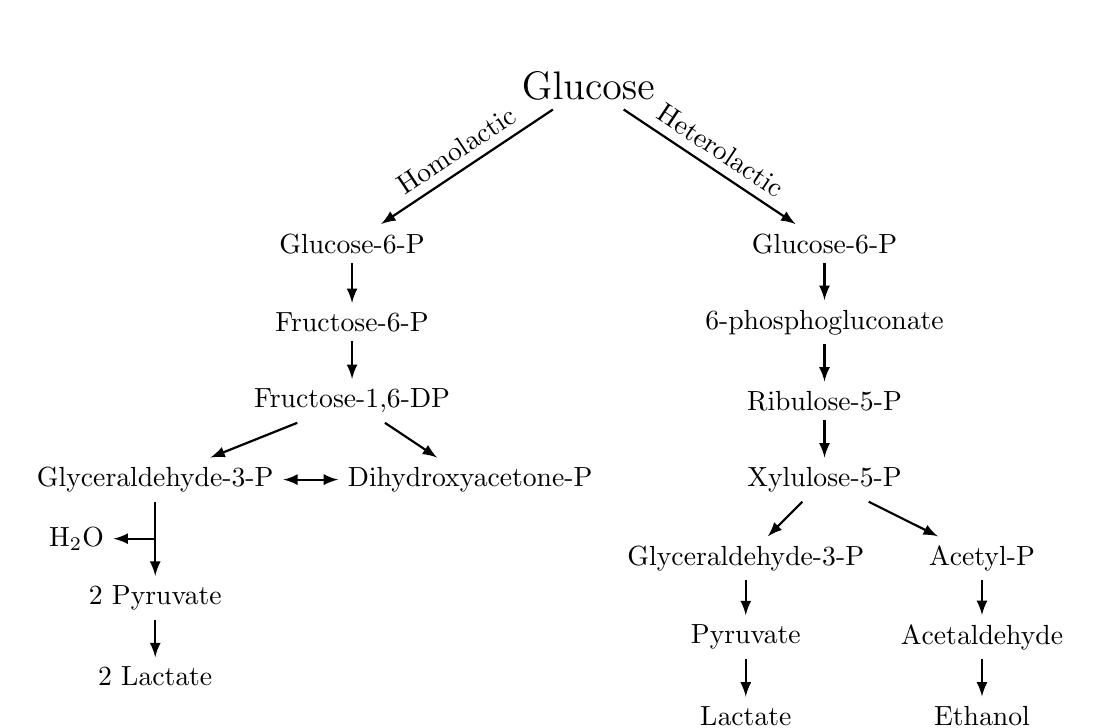
\begin{tikzpicture}[
        node distance=2cm,
        compound/.style={draw=none},
        arrow/.style={->, >=latex, thick},
        pathway_label/.style={sloped, above}
    ]
    
    % Main glucose node with larger font
    \node[compound] (glucose) at (0,0) {\Large Glucose};
    
    % Nodes for the pathways
    \node[compound] (g6p1) at (-3,-2) {Glucose-6-P};
    \node[compound] (g6p2) at (3,-2) {Glucose-6-P};
    
    % Path labels with arrows and text above
    \draw[arrow] (glucose) -- node[sloped, above] {Homolactic} (g6p1);
    \draw[arrow] (glucose) -- node[sloped, above] {Heterolactic} (g6p2);
    
    % Homolactic pathway
    \node[compound] (f6p) at (-3,-3) {Fructose-6-P};
    \node[compound] (f16dp) at (-3,-4) {Fructose-1,6-DP};
    \node[compound] (g3p) at (-5.5,-5) {Glyceraldehyde-3-P};
    \node[compound] (dhap) at (-1.5,-5) {Dihydroxyacetone-P};
    \node[compound] (pyr1) at (-5.5,-6.5) {2 Pyruvate};
    \node[compound] (lac1) at (-5.5,-7.5) {2 Lactate};
    
    % Heterolactic pathway
    \node[compound] (6pg) at (3,-3) {6-phosphogluconate};
    \node[compound] (r5p) at (3,-4) {Ribulose-5-P};
    \node[compound] (x5p) at (3,-5) {Xylulose-5-P};
    \node[compound] (g3p2) at (2,-6) {Glyceraldehyde-3-P};
    \node[compound] (ap) at (5,-6) {Acetyl-P};
    \node[compound] (pyr2) at (2,-7) {Pyruvate};
    \node[compound] (acet) at (5,-7) {Acetaldehyde};
    \node[compound] (lac2) at (2,-8) {Lactate};
    \node[compound] (eth) at (5,-8) {Ethanol};
    
    % Rest of the arrows for homolactic pathway
    \draw[arrow] (g6p1) -- (f6p);
    \draw[arrow] (f6p) -- (f16dp);
    \draw[arrow] (f16dp) -- (g3p);
    \draw[arrow] (f16dp) -- (dhap);
    \draw[<->, >=latex, thick] (g3p) -- (dhap);
    
    % Draw the vertical arrow from g3p to pyr1
    \draw[arrow] (g3p) -- (pyr1);
    \draw[arrow] (pyr1) -- (lac1);
    
    % H2O label with arrow coming from the vertical path
    \node[compound] (h2o) at (-6.5,-5.75) {H\textsubscript{2}O};
    \draw[arrow] (-5.5,-5.75) -- (h2o);
    
    % Arrows for heterolactic pathway
    \draw[arrow] (g6p2) -- (6pg);
    \draw[arrow] (6pg) -- (r5p);
    \draw[arrow] (r5p) -- (x5p);
    \draw[arrow] (x5p) -- (g3p2);
    \draw[arrow] (x5p) -- (ap);
    \draw[arrow] (g3p2) -- (pyr2);
    \draw[arrow] (ap) -- (acet);
    \draw[arrow] (pyr2) -- (lac2);
    \draw[arrow] (acet) -- (eth);
    
    \end{tikzpicture}
    \caption{Generalized scheme for the fermentation of glucose in lactic acid bacteria.}
    \label{fig:L8-lactic_acid_fermentation}
\end{figure}

\subsubsection*{Microbial Interference}
\textbf{Microbial interference} is a non-specific control that inhibits certain microbes through competition with natural flora. Relying on high interfering populations, mechanisms include \textbf{nutrient competition}, adverse \textbf{environmental changes}, and \textbf{attachment site competition} \cite*{L8-MicroInFood}.

\subsubsection{Mechanisms of antibiosis mediated by lactic acid bacteria}
\textit{Lactic acid bacteria} provide \textbf{biopreservation} via organic acids, hydrogen peroxide, diacetyl, reuterin, and bacteriocins, inhibiting pathogens in foods. \textbf{Microguard}, a product from \textit{P. freudenreichii} fermentation, is GRAS-approved in U.S. cottage cheese to prevent gram-negative bacteria and molds \cite*{L8-MicroInFood}.

\subsubsubsection*{Organic acids, acetaldehyde and ethanol as an Antimicrobial}
Organic acids like \textbf{lactic-, acetic-}, and \textbf{propionic} acids from lactic acid bacteria disrupt bacterial membranes and inhibit \textbf{transport}. \textbf{Acetic acid} is most effective, followed by \textbf{propionic}, targeting fungi and bacteria, while acetaldehyde and ethanol play minor roles due to low inhibitory concentrations \cite*{L8-MicroInFood}.

\subsubsubsection*{Hydrogen Peroxide as an Antimicrobial}
\textbf{Hydrogen peroxide} from lactic acid bacteria can inhibit microorganisms via oxidation of \textbf{lipids and proteins}. It may also activate milk's lactoperoxidase system, enhancing antimicrobial effects. However, the impact in vivo remains unclear due to breakdown by flavoproteins and peroxidases \cite*{L8-MicroInFood}.

\subsubsubsection*{Carbon Dioxide as an Antimicrobial} 
\textbf{Carbon dioxide} from heterolactic fermentation can create an anaerobic environment, inhibit aerobic microorganisms by impacting cell membranes, and lower pH. Low CO$_2$ levels may stimulate some bacteria; it also forms the characteristic "eyes" in Swiss cheese \cite*{L8-MicroInFood}.

\subsubsubsection*{Diacetyl as an Antimicrobial} 
\textbf{Diacetyl}, produced in citrate metabolism, contributes to butter's aroma and flavor and is generated by \textit{Leuconostoc}, \textit{Lactococcus}, \textit{Pediococcus}, and \textit{Lactobacillus}. Sensitive to Gram-negative bacteria, yeasts, and molds, it may inhibit arginine utilization but is rarely at effective antibacterial levels in food \cite*{L8-MicroInFood}.

\subsubsubsection*{Reuterin as an Antimicrobial} 
\textbf{Reuterin}, produced by \textit{Lactobacillus reuteri} during anaerobic growth on glucose and glycerol, exhibits broad antimicrobial effects against viruses, fungi, protozoa, and bacteria. Its primary mode of action is believed to be the inhibition of ribonucleotide reductase \cite*{L8-MicroInFood}.

\subsubsubsection*{Bacteriocins in Food Fermentation}
\textbf{Bacteriocins}, extracellular products of lactic acid bacteria, are ribosomally synthesized with a narrow bactericidal range, targeting mostly gram-positive cells due to their action on the cytoplasmic membrane. They inhibit pathogens and spoilers such as \textit{Listeria monocytogenes} and \textit{Clostridium} spp.. Bacteriocin-producing strains may enhance food safety as adjuncts in starter cultures. Activity is pH-dependent, and production may involve engineered strains with enhanced properties. Unlike antibiotics, bacteriocins are digested by enzymes, reducing residual effects \cite*{L8-MicroInFood}.

\subsubsubsection*{Class I Bacteriocins (Lantibiotics)}
\textbf{Lantibiotics}, such as nisin, are post-translationally modified bacteriocins from \textit{Lactococcus lactis} with GRAS status. Nisin exhibits broad activity against gram-positive bacteria, inhibits \textit{Clostridium} and \textit{Bacillus} spores, and aids in preserving cheese, canned foods, and baby foods. Its use stabilizes at low pH and is applied widely (50 countries). Another lantibiotic, lacticin 3147, effective at neutral pH, inhibits non-starter lactic acid bacteria in cheese, aiding in controlled flavor development and safety \cite*{L8-MicroInFood}.


\subsubsubsection*{Class II Bacteriocins}
\textbf{Class II} bacteriocins, especially pediocin-like, are effective against \textit{Listeria} and common in fermented meats. \textbf{Pediocin PA-1/AcH} and sakacin 674 inhibit \textit{L. monocytogenes}, enhancing food safety in vacuum-packed meats \cite*{L8-MicroInFood}.

\subsubsubsection*{Other Bacteriocins}
\textbf{\textit{Lb. sake}} strain CTC494 inhibits \textit{Listeria} in dry fermented sausage and is suggested as a \textbf{bioprotective culture} for meat products \cite*{L8-MicroInFood}.

\subsubsection*{Aspects to Consider in the Use of Bacteriocins/Bacteriocinogenic Cultures in Fermented Foods}
\textbf{Sensitivity to bacteriocins} is strain-dependent; resistance to nisin occurs at a frequency of 10$^{-6}$. Careful control is needed when using multiple bacteriocins to avoid cross-resistance. \textbf{Nisin} is the only bacteriocin with GRAS status, supported by 25 years of safe use, while others require premarket approval \cite*{L8-MicroInFood}.

\subsubsection{Fermented Foods}
\textbf{Fermented foods} are staples, made from milk, meat, cucumber, and cabbage, producing over 400 cheese varieties and various yoghurts, sausages, and pickles \cite*{L8-MicroInFood}.

\subsubsubsection*{Milk Products}
\textbf{Lactic fermentation} is essential for cheese production, often using starter cultures like \textit{L. lactis} subsp. \textit{lactis} and thermophilic strains. Secondary microflora enhance texture and flavor. Yogurt uses a 1:1 culture of \textit{S. thermophilus} and \textit{Lb. bulgaricu}s. Fermented milk drinks like kefir and kumiss contain beneficial bacteria, gaining popularity due to health benefits \cite*{L8-MicroInFood}.

\subsubsubsection*{Meat Products}
\textbf{Fermented sausages} are produced through lactic fermentation of comminuted meat mixed with fat, salt, curing agents, sugar, and spices. They are classified as dry ($a_w$ < 0.90) or semi-dry ($a_w$ $\approx$ 0.90-0.95), with fermentation temperatures below 22°C. Starter cultures, including \textit{Lb. sake} and \textit{Lb. curvatus}, ensure product quality and safety, reducing \textit{L. monocytogenes} counts during fermentation \cite*{L8-MicroInFood}.

\subsubsubsection*{Vegetable Products}
\textbf{Vegetable fermentation} in Europe includes olives, cucumbers, and cabbage, with raw vegetables having high microbial loads. Fermentations occur under conditions favoring lactic acid bacteria, which comprise only 0.15-1.5\% of the total microbial population. Fermented juices use pasteurized mash or juice with starter cultures like \textit{Lb. plantarum} and \textit{L. lactis} \cite*{L8-MicroInFood}.

\subsubsection*{Traditional Fermented Foods}
This section provides a detailed examination of various fermented foods from around the world. Table 1 offers an extensive overview, highlighting their origins, associated microorganisms, and substrates. For additional insights into products from Africa, India, Indonesia, and the Orient, please consult the original text \cite*{L8-MicroInFood}.

\subsubsection*{Developments in Food Fermentations}
Various fermented foods worldwide are produced through the metabolism of different substrates by microorganisms, yet their fermentation processes remain poorly understood. Future improvements in quality and safety will require deeper insights into microbial activities. While certain fermentations, such as those for cheese and yoghurt, are already reliable, further optimization is needed. Advances in lactic acid bacteria research, including metabolic engineering, promise to enhance flavor and functionality. However, consumer concerns about recombinant DNA technology must be addressed to maintain trust in fermented foods \cite*{L8-MicroInFood}.






